\documentclass[12pt,a4paper,oneside]{article}
\usepackage[utf8]{inputenc}
\usepackage{t1enc} % hyphenate accented chars
\usepackage[hungarian]{babel}
\usepackage{../fedlap}
\usepackage{fancyhdr} % elofej, elolab
\usepackage{graphicx}
\usepackage{datetime} % specify date format
\setcounter{secnumdepth}{3} % enable subsubsection

% hasonlitson a doc verziora
\addtolength{\voffset}{-1cm}

% cim
\csapat{nand}{39}
\konzulens{Bozóki Szilárd}
\datum{\todaynum}

% csapattagok
\taga{Berki Endre}{HQNHER}{berkiendre@gmail.com}
\tagb{Fodor Bertalan Ferenc}{H4T1UX}{foberci@gmail.com}
\tagc{Kádár András}{JFENWR}{arycika@gmail.com}
\tagd{Thaler Benedek}{EDDO10}{thalerbenedek@gmail.com}

\setlength{\headheight}{1.3em}
\setlength{\headsep}{2em}

% elofej, elolab
\fancyhf{}

\fancyhead[OL] { \tiny \leftmark{} }
\fancyhead[OR] { \tmpcsapat }

\fancyfoot[OR] { \thepage }
\fancyfoot[OL] { \tmpdatum }

\pagestyle{fancy}

% custom date format, according to customer request
% you have to use the \todaynum command instead of today,
% becouse babel overrides it, and I couldn't find a way to override
% it again. I was tempted to call this format \todaybozoki
\newcommand{\todaynum}{\the\year. \twodigit\month. \twodigit\day}


\usepackage{enumitem}
\usepackage{textcomp}
\usepackage[utf8]{inputenc}
\usepackage[T1]{fontenc}
\usepackage{longtable}

\begin{document}

\anyag{Continuity}
\fedlap

\newpage
\section{Követelmény, projekt, funkcionalitás}

\subsection{Követelmény definíció}

    \subsubsection{A program bemutatása, alapvető feladatai}
Az elkészített program egy nagymértékben logikai, kismértékben ügyességi játék, mely koncepcióját tekintve teljesen megfelel a Ragtime Games által fejlesztett Continuity játéknak\footnote{http://continuitygame.com/playcontinuity.html}. A játék során a játékos több pályán keresztül tesztelheti logikai és problémamegoldó készségét. Az előre kialakított pályákon az előrehaladás a keretek egymáshoz képest történő elmozdításával, a kereteken belül pedig egy figurával 2 dimenzióban végzett mozgással történik. Minden pálya egy $n*k$-s táblából áll, amin $n*k-1$ keret található. Az összeillő keretek között átjárás van, az üres hellyel szomszédos keretek átmozgathatóak az üres helyre. A játékos által irányított figurának a keretekben található kulcsokat kell összeszednie, hogy azzal a szintén a keretekben található ajtót kinyitva a pályát teljesítse.

    \subsubsection{Felhasználói felület}
A kész program grafikus felhasználói felülettel rendelkezik, melyen az indítással és működéssel kapcsolatos funkciók egy menüsoron keresztül érhetőek el, egér vagy billentyűzet segítségével. Maga a játék kizárólag billentyűzettel irányítható.

    \subsubsection{A program futtatásának követelményei}
A program futtatásához szükséges a futtató számítógépre telepített Java Runtime Environment (JRE), mely ingyenesen beszerezhető a gyártó honlapjáról\footnote{http://java.com/en/download/index.jsp} a legtöbb platformra. A program hardware követelménye megegyezik az Oracle által meghatározott minimum-konfigurációval\footnote{http://www.java.com/en/download/help/sysreq.xml}, mely szükségessé tesz egy kompatibilis operációs rendszert (Windows, Linux), rendszertől függően 64-128 MB memóriát és hozzávetőlegesen 100 MB szabad helyet.

    \subsubsection{A program telepítése}
A program futtatásához a kész terméket csupán a futtató számítógép merevlemezére kell másolni, további telepítés vagy beállítás nem szükséges, amennyiben a futtató számítógép megfelel a futtatás követelményeinek.

    \subsubsection{A program fordítása}
A program fordításához szükség van a \texttt{javac} programra, mellyel a \texttt{*.java} fájlok lefordíthatóak, és a futtatható \texttt{jar} fájl elkészíthető.
    
\subsection{Projekt terv}

    \subsubsection{Fejlesztőeszközök, erőforrások}
	A csapat választása az Eclipse\footnote{http://eclipse.org/} fejlesztői rendszerre esett, mert a java világ egyik legelterjedtebb, keresztplatformos IDE megoldása, melyet a csapat minden tagja használt már korábban. UML modellezéshez, diagramok készítéséhez a Visual Paradigm Community Edition\footnote{http://www.visual-paradigm.com/} kiadását fogjuk használni.
A dokumentáció \LaTeX -ben készül, mely segítségével nyomtatásban jól kinéző dokumentumok készíthetőek, valamint a forrásfájlok könnyen verziókezelhetőek. A végső fájlokat PDF formátumba fordítjuk, majd ezt kinyomtatva adjuk be. A verziókezelést és a felmerülő problémák megoldását a GitHub\footnote{https://github.com/} online és ingyenes felületen keresztül oldjuk meg.

    \subsubsection{A fejlesztőcsapat tagjai, feladatai}
	\begin{center}
	\begin{tabular} {| l | c | }
		\hline
		Név & Feladatok\\
		\hline
		Thaler Benedek & csapatvezetés, dokumentáció, diagramok készítése, kódírás \\ 
		\hline
		Berki Endre & dokumentáció, diagramok készítése, kódírás \\
		\hline
		Fodor Bertalan & dokumentáció, diagramok készítése, kódírás \\
		\hline
		Kádár András & dokumentáció, diagramok készítése, kódírás \\
		\hline
	\end{tabular}
	\end{center}
	A feladatkörök, beosztások változhatnak a személyes időráfordítástól függően. A feladatok elosztásakor a fő szempont, hogy a feladatokat egyenlően tudjuk elosztani, így minimalizálva az egy emberre eső terhelés mértékét.

    \subsubsection{Kommunikációs modell}

	A tárgy keretében, a projektbe válogatott csoport tagjai előzetesen ismerték egymást, az előzetes ismeretség megkönnyíti az együttműködést és a hatékony munkavégzést. A munkavégzést további kommunikációt segítő programok támogatják.
	A kommunikáció megszervezése elsődleges fontosságú, így minél előbb próbáltuk felépíteni a kommunikációs hálózatot. Két részre oszthatóak a felhasznált kapcsolatteremtési formák, egyik a szinkron, másik az aszinkron kommunikáció. Szinkron kommunikációban lehetséges a folyamatos kommunikálás, azonnali reagálással egymás ötleteire, kérdéseire. Látható, hogy minden csapattag egyidejű bevonása a kommunikációba költséges és gyakran felesleges, ezért az ilyen megbeszéléseket minimálisra szorítjuk. Emellett fontos az asszinkron kommunikációs eszközök használata, melyek segítségével a csapattagok egymás elérhetőségétől függetlenül üzenhetnek egymásnak. Ez a fajta kommunikáció megfelelő a státusz jelentések számára, valamint az előrehaladás követésére vagy a feladatok kiadására.
	A csapatmunka számára a legfontosabb rendszer a GitHub által biztosított tároló\footnote{https://github.com/nandinc/Continuity}. Ez egy összetett rendszer, amely többféle lehetőséget biztosít számunkra:
	\begin{description}
		\item[Git verziókezelés:]
			A dokumentum és kódkészítés folyamatában lehetőséget nyújt, hogy többen dolgozhassanak együttesen a projekten, mindig mindenki a legfrissebb verziót érje el, manuális változáskövetés nélkül. Ezen felül segít nyomonkövetni a csapattagok munkáját egy részletes napló segítségével. % commit szó nem szerepelhet
		\item[Hibajegy nyilvántartó:] % issue tracker nem szerepelhet
			A feladatok kiosztása hibajegyeken kereszül történik. Egy-egy hibajegy addig marad nyitva, ameddig a hozzárendelt csapattag a feladatot el nem készíti és azt egy másik le nem ellenőrzi. Ezután a hibajegy lezárásra kerül, de a rendszerben marad, így későbbi probléma esetén újra megnyitható. A hibajegyek használatával a csapatvezető könnyen rendelhet feladatokat a csapattagokhoz, valamint lehetőség van egy feladat önkéntes elvállalására is. A hibajegyben a feladója pontosan leírja a feladatot, feltünteti a felhasználható forrásokat és kiköti, hogy milyen körülmények teljesítése mellett zárható le a jegy.
		\item[Wiki:]
			Az értekezletek eredményeit, a csapattagok által készített segédleteket, fejlesztési irányelveket tároljuk itt.
	\end{description}
	Ezeken felül kommunikáció lehetséges a heti rendszerességgel tartott megbeszéléseken, Skype-konferencia formájában és egyéb személyes találkozókon. A teljes projekt döntéseit érintő kérdések megbeszélése valamint tervezési feladatok kidolgozása ezen szinkron kommunikációs formákban praktikusabb.

	\begin{figure}[ht]
		\begin{center}
			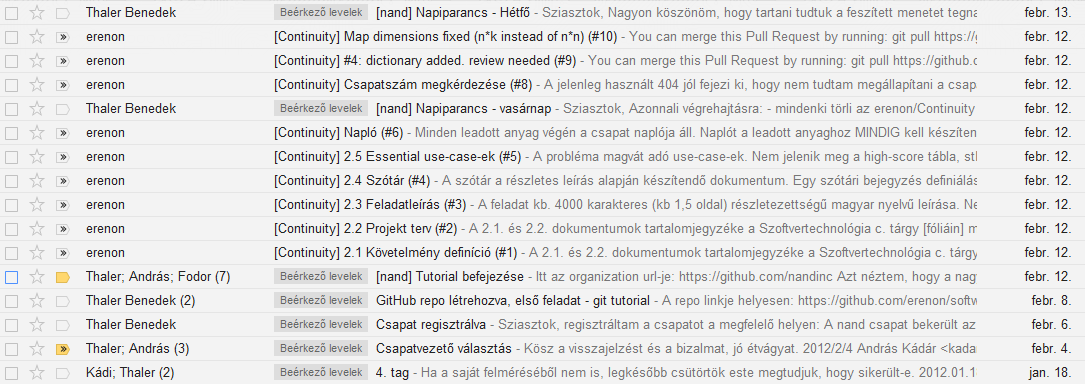
\includegraphics[scale=0.5]{resources/02/levlista.png}
			\caption{Levelezőlista}
		\end{center}
	\end{figure}
	
	\begin{figure}[ht]
		\begin{center}
			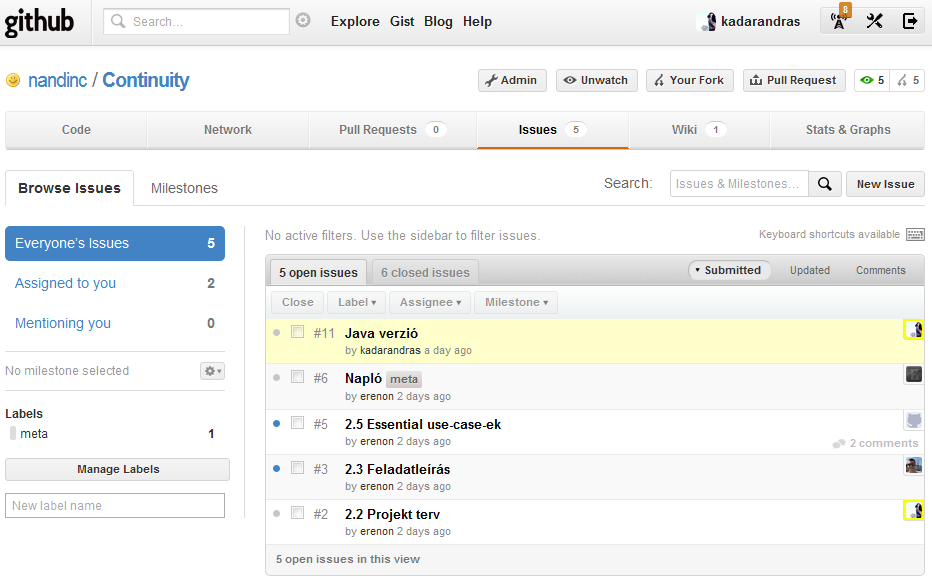
\includegraphics[scale=0.5]{resources/02/issues.png}
			\caption{A GitHub által biztosított hibajegykezelő}
		\end{center}
	\end{figure}

    \subsubsection{Fejlesztési mérföldkövek}

	\begin{description}
		\item[Szkeleton:] Az első fontosabb mérföldkő, a program vázának megalkotása, a program modelljének megtervezése, annak helyességének és részletességének ellenőrzése. A tervezési folyamat során fontos a gondos és odafigyelő döntéshozás, mert ezek a már elkészült program minőségét nagyban befolyásolják. Általánosságban igaz, hogy az itt elkövetett tervezői hibák később sokkal nagyobb erőfeszítéssel javíthatóak.
		
		\item[Prototípus:] A második mérföldkő a program működőképes változata, ami még a grafikát nem tartalmazza. A mérföldkő elérése a program egészének tesztelését teszi lehetővé. A fejlesztés ezen része lezárultnak tekinthető, ha az algoritmusok és adatszerkezetek, valamint az osztályhierarchia eléri végleges formáját, így egy a grafikus felülettől független programot alkot.
		
		\item[Grafikus felület:] A harmadik és egyben utolsó mérföldkövet a grafikus felület befejezése jelenti. A már kész, jól működő prototípust megfelelően felhasználva, azt meg nem bontva kell rá felépíteni a grafikus felületet. A felület fontos jellemzője az intuitív elrendezés, a felhasználó barát működés és könnyű használhatóság.
	\end{description}

    \subsubsection{Határidők}
	\begin{center}
	\begin{tabular}{| l | l | }
		\hline
		febr. 10. & 14 h -- csapatok regisztrációja\\
		\hline
		febr. 20. & Követelmény, projekt, funkcionalitás -- beadás\\
		\hline
		febr. 27. & Analízis modell kidolgozása 1. -- beadás\\
		\hline
		márc. 5. & Analízis modell kidolgozása 2. -- beadás\\
		\hline
		márc. 12. & Szkeleton tervezése -- beadás\\
		\hline
		márc. 19. & Szkeleton -- beadás\\
		\hline
		márc. 26. & Prototípus koncepciója -- beadás\\
		\hline
		ápr. 2. & Részletes tervek -- beadás\\
		\hline
		ápr. 16. & Prototípus -- beadás\\
		\hline
		ápr. 23. & Grafikus felület specifikációja -- beadás\\
		\hline
		máj. 7. & Grafikus változat -- beadás\\
		\hline
		máj. 11. & Összefoglalás -- beadás\\
		\hline
	\end{tabular}
	\end{center}

    \subsubsection{Átadás}
	A dokumentációt nyomtatott formában minden héten a konzulensnek le kell adni a konzultáció időpontjában. Ezen kívül a három mérföldkő alkalmával a programkódok is bemutatásra kerülnek az ezen célra kijelölt laboratórium gépeinél. A végső átadás a félév végeztével az aktualizált dokumentációval és forráskódokkal feltöltésre kerül a tárgy honlapjára\footnote{http://www.iit.bme.hu/hercules}.
%
%   \subsubsection{Kockázatelemzés}
%	\begin{description}
%	\item[Valószínűségek osztályozása:] \hfill \\
%		\begin{description}
%			\item[Alacsony] Közelítőleg 0-20\%-os eséllyel bekövetkező esemény
%			\item[Közepes] Közelítőleg 20-50\%-os eséllyel bekövetkező esemény
%			\item[Biztos] Közelítőleg 50-100\%-os eséllyel bekövetkező esemény
%		\end{description}
%	\item[Hatások osztályozása:] \hfill \\
%		\begin{description}
%			\item[Elhanyagolható] Az esemény bekövetkezése nem okoz különösebb problémát, az esetleges javítása nem igényel komoly munkálatokat.
%			\item[Enyhe] Az esemény bekövetkeztével okozott kár legfeljebb néhány munkaórával javítható, visszaállítható.
%			\item[Közepes] A csapat több tagjának összehangolt munkáját igénylő probléma, melynek megoldása komolyabb erőfeszítéseket igényel. Ezen változtatások már hatással lehetnek a heti ütemtervre, és a fejlesztőcsapat közös megbeszélését igényelhetik.
%			\item[Komoly] A projekt sikeres kimenetelét vagy a csapat integritását fenyegető esemény, mely alapvető változtatásokkal jár. Az ilyen jellegű probléma a csapat azonnali tanácskozását igényli.
%		\end{description}
%	\end{description}
%
%	Eseménytáblázat:
%	\begin{center}
%		\begin{tabular}{| l | l | l |}
%			\hline
%			\textbf{Esemény}			&	\textbf{Valószínűség}	&	\textbf{Hatás}\\
%			\hline
%			Specifikációváltozás			&	Biztos				&	Enyhe\\
%			\hline
%			Javítandó heti beadandó		&	Közepes			&	Enyhe\\
%			\hline
%			Sikertelen heti beadandó		&	Alacsony			&	Közepes\\
%			\hline
%			Csapattag kiválás			&	Alacsony			&	Komoly\\
%			\hline
%			Csapattag betegsége, távolléte	&	Alacsony			&	Közepes\\
%			\hline
%			Hardvermeghibásodás		&	Alacsony			&	Elhanyagolható\\
%			\hline
%			Szoftvermeghibásodás		&	Közepes			&	Enyhe\\
%			\hline
%			Határidorol lecsúszás		&	Alacsony			&	Közepes\\
%			\hline
%			Tanácskozásról hiányzás		&	Közepes			&	Közepes\\
%			\hline
%		\end{tabular}
%	\end{center}
%
   \subsubsection{Egyéb fontos megjegyzések}
	A fejlesztés lefordítása és bemutatása a HSZK laborjaiban történik, így a program forráskódjának kompatibilisnek kell lennie a Java Development Kit ennek megfelelő korábbi verziójával. A maximális kompatibilitás elérése érdekében a fejlesztés is pontosan ezeken a verziószámú platformokon történik majd, azaz 6-os Java JDK és 1.6.0 verziójú JRE kerül felhasználásra.

    \subsubsection{Szükséges dokumentációk}
	\begin{enumerate}
	\item Követelmény, projekt, funkcionalitás
	\item Analízis modell kidolgozása 1.
	\item Analízis modell kidolgozása 2.
	\item Szkeleton tervek
	\item Szkeleton
	\item Prototípus koncepciója
	\item Részletes tervek
	\item Prototípus
	\item Grafikus felület specifikációja
	\item Grafikus változat
	\end{enumerate}
 
\subsection{Feladatleírás}

	A feladat a Continuity\footnote{http://continuitygame.com/playcontinuity.html} nevű logikai játék elkészítése. A játékos feladata az általa irányított pálcikaembert (továbbiakban: Stickman) a kétdimenziós térben úgy navigálni, hogy az megszerezze a pályán elhelyezett összes kulcsot, majd átmenjen a piros ajtón, így jutva a következő szintre. A játék különlegessége abban rejlik, hogy a pályák egy puzzle-hoz hasonlóan kis elemekből épülnek fel, melyek bizonyos szabályok szerint a játékos által átrendezhetőek.
	
	A felhasználó a játék elindításakor a főképernyővel találja szemben magát, ahol lehetősége van új játékot kezdeményezni vagy -- amennyiben már korábban is játszott -- a már megkezdett játékot folytatni.
	
	A játék szintekből áll, minden szinthez egy pálya tartozik. A pályák keretekből (csempékből) épülnek fel, melyek táblázatszerűen helyezkednek el. Ez a táblázat -- pályától függően -- tetszőlegesen széles vagy magas lehet, azonban mindig van benne pontosan egy üres cella, ami arra szolgál, hogy a kereteket tologatni lehessen. Csak az üres cella melletti keretek tolhatóak át az üres helyre, amennyiben a Stickman nem lóg ki a mozgatandó keretből. Ugyanis előfordulhat, hogy emberünk egy másik keretbe átlóg, ekkor a keret elmozdítása a szétszakítását eredményezné -- erre azonban egy pusztán logikai játékban nincs lehetőség.
	
	%Egy keret mozgatásához két feltételnek szükséges teljesülnie. Ez akkor tehető meg, ha egyrészről van mellette üres hely (ide lehet a keretet tolni, kereteket felcserélni nem lehet), illetve másrészről ha Stickman nem éppen a keret határán tartózkodik, azaz csak félig a mozgatandó keretben.
	
	Keretek mozgatására akkor nyílik lehetőség, amikor a játékos pálya nézetben van; ez a nézet töltődik be közvetlenül a pálya elindítása után. Ebben a nézetben a játékos a teljes pályát átlátja, az összes keret megjelenik, és Stickman mozgása szüneteltetve van.
Stickman mozgatására a játékosnak a közeli nézetben van lehetősége. Ide a pálya nézetből lehet jutni a szóköz billentyű lenyomásával (ugyanígy lehet vissza is menni), és ekkor a képernyőn csak Stickman, valamint az aktuális -- nagyjából egy keret nagyságú -- környezete jelenik meg.
	
	Stickmant a játékos irányítja a billentyűzetének kurzorai segítségével. Amíg akadályba nem ütközik, mehet jobbra--balra, illetve ugorhat is, valamint ha elfogy alóla a talaj, akkor esni kezd. A mozgást a keretek közti átjárást szabályzó speciális szabályok nehezítik. Ha Stickman kerethatárra érkezik, akkor két eset lehetséges. Amennyiben a keretek az adott oldalon átjárhatóak, akkor szabadon folytathatja útját a másik keretbe. Ha az érintett keretek nem átjárhatóak vagy az érintett irányban már nincs több keret, akkor ha oldalsó határról van szó, visszapattan (a kerethatár akadályként viselkedik), ha alsóról, akkor a játékos kiesik. Két keret akkor átjárható, ha a csatlakozó szélükön a tereptárgyak elhelyezkedése megegyezik.
	
	A játékos kiesése azzal jár, hogy Stickman visszakerül az utolsó mentési ponthoz (ellenőrző pont). Ilyen mentési pont Stickmannek a pályához tartozó kiindulási helye, vagy a legutóbb megszerzett kulcs helye. Amennyiben a játékot elmentjük, majd később folytatjuk, akkor is a mentési pont lesz a kiinduló pont.
	
	Játék közben mind a pálya nézetből és a közeli nézetből az escape gomb megnyomásával elő lehet hozni egy menüt, mellyel menteni lehet az aktuális állapotot, illetve vissza lehet térni a főképernyőre.
	% Restart levelt és Skip Levelt ugye nem akarjuk megvalósítani?
	
	A pályán különböző kulcsok vannak elhelyezve, melyeket a játékosnak az előrehaladáshoz meg kell szereznie. Ezt úgy teheti meg, ha Stickmant vezetve megérinti ezeket, azaz elhalad előttük. Ha megszerezte az összes kulcsot, akkor a pályán elhelyezett ajtót kell célba vennie. Az ajtó előtt való elhaladáskor -- amennyiben a játékosnál van az összes kulcs -- az ajtó automatikusan kinyílik és a pálya teljesítésre kerül. Amennyiben a játékos még nem szerezte meg az összes kulcsot, az ajtó kinyitása nem lehetséges.
	
	Pálya teljesítése esetén egy átvezető képernyő után rögtön sor kerül a következő pálya automatikus betöltésére. Amennyiben több pálya már nem létezik, úgy egy gratuláló megjegyzés után a főképernyőre tudunk visszajutni.

\subsection{Szótár}

\begin{description}

    \item[Játékos] A programot kezelő felhasználó
    \item[Számítógép] A programot futtató számítógép, mely megfelel a futtatás követelményeinek
    \item[Monitor] A \emph{számítógéphez} csatlakoztatott képernyő, melyen a futtatott program megjelenik
    \item[Pálya] A játékban való előrehaladás egysége. Minden pálya egy $n*k$ méretű táblázatból áll, melyben $n*k-1$ előre meghatározott \emph{keret} előre meghatározott helyen található. A fennmaradó helyen egy \emph{üres keret} található.
    \item[Keret] Egy \emph{pálya} több keretből áll. Minden keret \emph{elem}eket tartalmaz. A \emph{Keretek} egymáshoz képest \emph{átrendez}hetőek. Két érintkező keret között egyértelműen megállapítható, hogy \emph{átjárhatóak}-e. Amennyiben \emph{Stickman} a keret alsó szélét érinti úgy, hogy az \emph{aktuális keret} nem \emph{átjárható} az alatta található kerettel, vagy nincs alatta keret, akkor \emph{Stickman} \emph{kiesik}.
    \item[Átjárható] Két \emph{keret} átjárható, ha az érintkező oldalukon a \emph{platform}ok elhelyezkedése megegyezik.
    \item[Aktuális keret] Az a \emph{keret}, amiben a játékos lába tartózkodik.
    \item[Üres keret] Az üres keret biztosít lehetőséget arra, hogy vele helyet cserélve a \emph{keret}ek átrendezhetőek legyenek. Az üres keret nem rendelkezik vizuális reprezentációval, csupán távtartó funkciója van.
    \item[Elem] Egy \emph{keret} dinamikus vagy statikus alkotórészei; \emph{Stickman}, \emph{kulcs}, \emph{ajtó}, \emph{platform}.
    \item[Stickman] A játékban a \emph{játékos} által irányított emberformájú figura.
    \item[Kulcs] A \emph{játékos} által \emph{megszerez}hető \emph{elem}. A \emph{pályá}n található összes kulcs megszerzése után van lehetőség az \emph{ajtó} \emph{kinyit}ására.
    \item[Ajtó] Olyan \emph{elem}, melyet \emph{kinyit}va a pálya \emph{teljesít}ettnek tekinthető.
    \item[Platform] Olyan \emph{elem}, mely meghatározza a \emph{keret} bejárható és nem bejárható részeit. Egy 2 dimenziós objektum, melyen a \emph{játékos} irányítása szerint \emph{Stickman} mozoghat.
    \item[Megszerez] \emph{Stickman} egy megszerezhető \emph{elem}et megszerez, ha azt megérinti, azaz elhalad előtte. Egy \emph{elem} csak egyszer szerezhető meg, el nem veszíthető.
    \item[Kinyit] \emph{Stickman} az \emph{ajtó}t kinyithatja, ha \emph{megszerez}te a \emph{pályá}n található összes \emph{kulcs}ot. A kinyitás módja az ajtó megérintése. A kinyitás bekövetkeztekor a \emph{pálya} \emph{teljesít}ettnek tekinthető.
    \item[Teljesít (pályát)] A \emph{játékos} teljesíti a \emph{pályát}, ha \emph{kinyit}ja a pálya \emph{ajtaját}. Teljesítés után a \emph{következő pályá}ra léphet.
    \item[Kiesik] Ha \emph{Stickman} kiesik, akkor eltűnik, majd megjelenik az utolsó érintett \emph{ellenőrzőpont}nál
    \item[Ellenőrzőpont] Ellenőrzőpont a \emph{pálya} \emph{kezdőpont}ja, valamint minden \emph{kulcs} helye.
    \item[Kezdőpont] A \emph{pálya} egy pontja, ahol \emph{Stickman} először megjelenik a pálya betöltésekor.
    \item[Átrendez] Egy \emph{keret} átrendezhető, ha mellette \emph{üres keret} található és \emph{Stickman} csupán egy keretben jelenik meg. Ekkor a két \emph{keret} helye felcserélhető. Az átrendezést a \emph{játékos} vezérli.
    \item[Nézet] Meghatározza, hogy a \emph{játékos} az összes \emph{keret}et, (\emph{pálya nézet}) vagy csak a \emph{Stickman}t és közvetlen környezetét (\emph{közeli nézet}) lássa.
    \item[Pálya nézet] A \emph{játékos} az összes \emph{keret}et látja, és \emph{átrendez}ést kezdeményezhet.
    \item[Közeli nézet] A \emph{játékos} csak \emph{Stickman}t és -- nagyjából egy \emph{keret}nyi -- közvetlen környezetét látja, valamint vezérelheti a \emph{Stickman} mozgását.
    \item[Nézetváltás] A \emph{játékos} utasítására bármikor nézetváltás történhet, mely bekövetkeztekor a grafikus felület ráközelít az \emph{aktuális keret}re (\emph{Pálya nézet}ről \emph{Keret nézet}re váltás esetén) vagy eltávolodik az a \emph{Aktuális keret}ről az összes keret nézetére (\emph{Pálya nézet})
    \item[Nézetváltás] A \emph{játékos} utasítására bármikor nézetváltás történhet, mely bekövetkeztekor \emph{pálya nézet}ről \emph{közeli nézet}re váltás esetén a grafikus felület ráközelít \emph{Stickman}re, fordított esetben eltávolodik \emph{Stickman}től és a teljes pályát mutatja (\emph{pálya nézet}).
    \item[Következő pálya] Az aktuális \emph{pálya} után soron következő \emph{pálya} a \emph{pályalistá}ban.
    \item[Pályalista] A program által tartalmazott összes \emph{pálya} egy előre definiált sorrendben.

\end{description}


\clearpage
\subsection{Essential use-case-ek}
	\subsubsection{Essential use-case diagram}
	
		\begin{figure}[h!]
			\begin{center}
				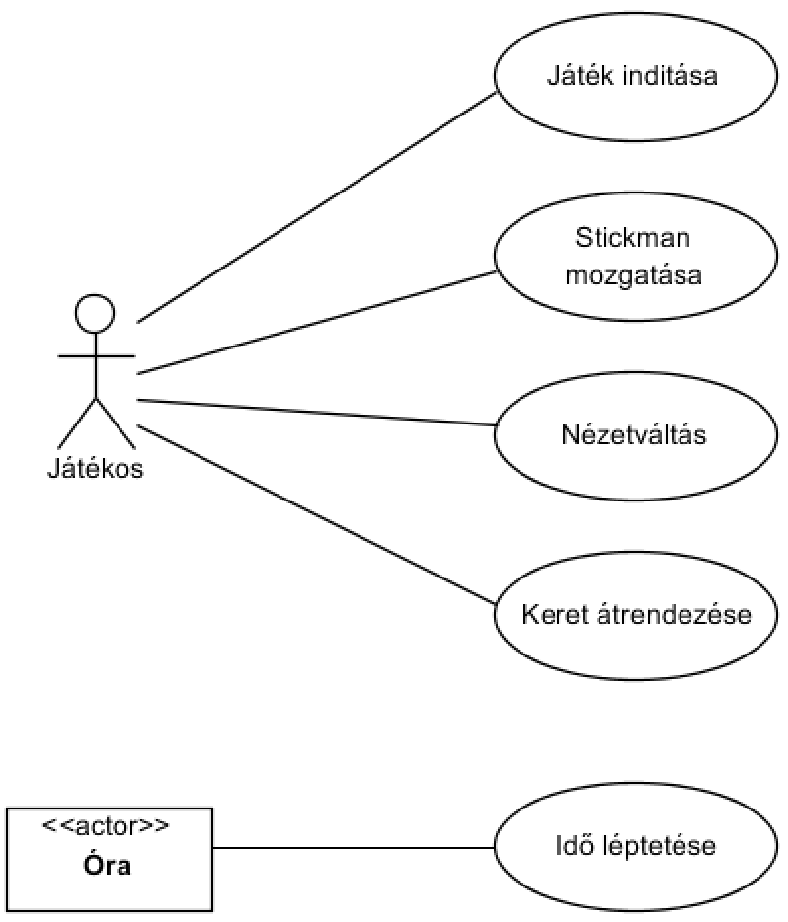
\includegraphics[scale=0.4]{resources/02/essential_use_cases.png}
				\caption{Essential use-case-ek}
			\end{center}
		\end{figure}
						
	\subsubsection{Essential use-case-ek leírása}
	
		\begin{description}
		
		\item[Játék indítása] \hfill \\
			A játékos folytatja a játékot, a legutóbbi, még teljesítetlen pálya töltődik be.
		\item[Stickman mozgatása]\hfill \\
			A játékos vezérli a figura (Stickman) mozgását. Stickman mozgatása a leütött billentyűnek megfelelően fog megtörténni.
		\item[Nézetváltás]\hfill \\
			A játékos a megfelelő billentyű lenyomásával nézetet vált (közeli és pálya nézet).
		\item[Keret átrendezése]\hfill \\
			Pálya nézetben a játékos a megfelelő billentyűkkel átrendezheti a pályát alkotó keretek helyzetét.
		\item[Idő léptetése]\hfill \\
			Egy számítógép által vezérelt actor végzi. Meghatározott időközönként jelzi az idő múlását, mely közeli nézetben Stickman vertikális pozícióját befolyásolhatja.
		\end{description}

\subsection{Napló}
% The diary generator uses the following comments to identify the beginning and the ending of the generated diary
% The following content is auto generated, please do NOT modify, edit the related shared document instead.
%GENERATOR:DIARY
    \begin{center} 
        \begin{tabular}{| l | p{1.9cm} | p{2.6cm} | p{6.1cm} |}
            \hline
                Kezdet & Időtartam & Résztvevők & Leírás \\
            \hline \hline 
2012. 02. 04. 20:00 & 1 óra & Thaler, Fodor & Csapat meeting\\ \hline
2012. 02. 06. 00:00 & 5 óra & Thaler & Csapat menedzsment, kommunikáció, feladatkiadás\\ \hline
2012. 02. 08.  09:20 & 1 óra & Thaler & Git tutorial elkészítése\\ \hline
2012. 02. 10. 19:50 & 4 óra & Kádár & Github telepítése, tutorial használata, saját repository\\ \hline
2012. 02. 11. 13:00 & 3 óra & Berki & Git telepítés, konfigurálás, tutorial végrehajtása\\ \hline
2012. 02. 11. 18:00 & 2 óra & Thaler & Continuity játék tanulmányozása\\ \hline
2012. 02. 11. 18:20 & 2 óra & Berki & Continuity játék tanulmányozása\\ \hline
2012. 02. 11. 20:00 & 2 óra & Fodor & Continuity játék tanulmányozása\\ \hline
2012. 02. 11. 21:00 & 2 óra & Kádár & Continuity játék tanulmányozása\\ \hline
2012. 02. 12. 04:40 & 3 óra & Thaler & Latex keret és Követelmény definíció elkészítése\\ \hline
2012. 02. 12. 12:00 & 4 óra & Kádár & Projekt terv elkészítése\\ \hline
2012. 02. 12. 17:00 & 4 óra & Fodor & Github ismerkedés, repository felállítás\\ \hline
2012. 02. 12. 6:40 & 4 óra & Thaler & Szótár elkészítése\\ \hline
2012. 02. 13. 22:15 & 2 óra & Berki & Essential use case diagram, leírások elkészítése\\ \hline
2012. 02. 14. 17:00 & 4 óra & Fodor & Feladatleírás\\ \hline
2012. 02. 14. 18:00 & 1 óra & Kádár & Projekt terv kiegészítése, véglegesítése\\ \hline
2012. 02. 15. 07:28 & 2 óra & Thaler & Projekt terv és Feladatleírás felülvizsgálata, kiegészítése\\ \hline
2012. 02. 15. 8:00 & 1.5 óra & Fodor, Kádár, Thaler & Konzultáció\\ \hline
2012. 02. 16. 10:00 & 3 óra & Kádár & Javadoc to Latex tool készítése\\ \hline
2012. 02. 16. 18:00 & 1 óra & Kádár & Wiki tutorial készítése, a dokumentáció generálóhoz.\\ \hline
2012. 02. 16. 23:00 & 1 óra & Fodor & Feladatleírás javítása\\ \hline
2012. 02. 17. 16:00 & 2 óra & Fodor & Latex fájl átnézése\\ \hline
2012. 02. 17. 21:00 & 1 óra & Fodor & Dokumentáció konzisztencia javítás\\ \hline
2012. 02. 18. 18:00 & 1 óra & Fodor & Javadoc to Latex tool átnézése\\ \hline
2012. 02. 18. 20:15 & 2 óra & Berki & Essential use case-ek véglegesítése, szerkesztése\\ \hline
2012. 02. 20. 08:00 & 1.5 óra & Kádár & Beadandó pdf dokumentum átnézése, nyomtatása\\ \hline

            \hline
        \end{tabular}
    \end{center}
%GENERATOR:DIARY

\newpage
\section{Analízis modell kidolgozása}

	\subsection{Objektum katalógus}
%GENERATOR:CLASS_RESPONSIBILITY
		\begin{description}
			\item[AbstractFrameItem] Alapértelmezett megvalósítása egy keretben lévő objektumnak.
			\item[Area] Területrészt leíró osztály. Összehasonlítható egy másik osztállyal, hogy fedik-e egymást.
			\item[DIRECTION] Irányokat jelöl a két dimenziós térben.
			\item[Door] Ajtó objektum, melyet ha megérint a Stickman arról esemény bocsát ki.
			\item[Frame] A pálya által alkotott táblázat egy cellája, amely elemeket tartalmaz. Ez felelős az elemek (Stickman) mozgatásáért kereten belül és között egyaránt. Két elem egy helyen való tartózkodásáról értesíti az elemeket (collision notify).
			\item[FrameItem] A keretben elhelyezkedő elemek által megvalósított iterfész, melyen keresztül a keret menedzselni tudja a benne lévő elemeket.
			\item[Game] A játékot reprezentáló objektum, amely kezeli az aktuális pályát.
			\item[Key] Kulcs elem, melyet megérintve a Stickman meg tud szerezni. Erről egy esemény küldésén keresztül értesíti a külvilágot.
			\item[Map] Számon tartja a pályán elhelyezett kulcsokat számát, valamint a már összegyűjtött kulcsok számát. Felelős a keretek mozgatásáért.
			\item[MapFactory] Felelős a pályák létrehozásáért, bennük a keretek és az elemek elhelyezéséért.
			\item[Platform] Olyan elem, mellyel nem tud a Stickman egy helyen tartózkodni, azaz korlátozza a Stickman mozgásterét.
			\item[PubSub] Üzenetközvetítő osztály, mely feliratkozásokat tart számon, és ha valakitől eseményt kap, arról értesíti az arra feliratkozottakat.
			\item[Stickman] A játékos által irányított figura, mely a pályán mozog.
			\item[Subscriber] Olyan interfész, melyen keresztül eseményeket lehet fogadni a PubSubtól.
			\item[Timer] Időzítésért felelős osztály, bizonyos időközönként kibocsát egy 'tick' eseményt az átadott PubSub objektumra.
		\end{description}
%GENERATOR:CLASS_RESPONSIBILITY	
	
	\subsection{Osztályok leírása}
	
%GENERATOR:CLASS_DESCRIPTIONS
		\subsubsection{AbstractFrameItem} Absztrakt osztály.
				 Alapértelmezett megvalósítása egy keretbe helyezett objektumnak.   Nyilvántartja a kereten belüli pozícióját, valamint hordoz  egy referenciát a tartalmazó keretre. 			\begin{description}


				\item[Ősosztályok] (nincs).
				\item[Interfészek] FrameItem.
				\item[Attribútumok]$\ $
					\begin{description}
						\item[\texttt{protected Area area}] A tartalmazó kereten belül elfoglalt pozíció 
						\item[\texttt{protected Frame frame}] A tartalmazó keret 
					\end{description}
				\item[Metódusok]$\ $
					\begin{description}
						\item[] (nincs)
					\end{description}
			\end{description}

		\subsubsection{Area}
				 Egy tetszőleges keret egy területét leíró osztály.  Ez az osztály elfedi, hogy egy keret valójában hány dimenziós,  valamint azt, hogy egy keret egy összefüggő ponthalmaza milyen   paraméterekkel írható le. 			\begin{description}


				\item[Ősosztályok] (nincs).
				\item[Interfészek] (nincs)
				\item[Attribútumok]$\ $
					\begin{description}
						\item[\texttt{private int height}] A terület magassága 
						\item[\texttt{private int width}] A terület szélessége 
						\item[\texttt{private int x}] A terület bal felső sarkának x eltolása 
						\item[\texttt{private int y}] A terület bal felső sarkának y eltolása 
					\end{description}
				\item[Metódusok]$\ $
					\begin{description}
%						\item[\texttt{public int getHeight()}] \hfill \\
						% TODO document getHeight
%						\item[\texttt{public int getWidth()}] \hfill \\
						% TODO document getWidth
%						\item[\texttt{public int getX()}] \hfill \\
						% TODO document getX
%						\item[\texttt{public int getY()}] \hfill \\
						% TODO document getY
						\item[\texttt{public boolean hasCollision(Area area)}] \hfill \\ Ellenőrzi, hogy a kapott Area objektummal van-e közös pontja.  A metódus feltételezi, hogy a két terület azonos keretben található. 
%						\item[\texttt{public void setHeight(int height)}] \hfill \\
						% TODO document setHeight
%						\item[\texttt{public void setWidth(int width)}] \hfill \\
						% TODO document setWidth
%						\item[\texttt{public void setX(int x)}] \hfill \\
						% TODO document setX
%						\item[\texttt{public void setY(int y)}] \hfill \\
						% TODO document setY
					\end{description}
			\end{description}

		\subsubsection{DIRECTION}
				 Enumeráció. Elfedi, hogy a játéktér hány dimenziós.  A tartalmazott elemek leírják az összes lehetséges irányt,   melybe a játékos mozoghat, vagy keretet cserélhet.  			\begin{description}


				\item[Ősosztályok] (nincs).
				\item[Interfészek] (nincs)
				\item[Attribútumok]$\ $
					\begin{description}
						\item[] (nincs)
					\end{description}
				\item[Metódusok]$\ $
					\begin{description}
						\item[] (nincs)
					\end{description}
			\end{description}

		\subsubsection{Door}
				 A pályák befejezésére szolgáló ajtót reprezentálja.  Ha a Stickman az összes kulcs birtokában megérinti,  a pálya teljesítésre kerül. 			\begin{description}


				\item[Ősosztályok] AbstractFrameItem $\rightarrow{}$ Door.
				\item[Interfészek] (nincs)
				\item[Attribútumok]$\ $
					\begin{description}
						\item[] (nincs)
					\end{description}
				\item[Metódusok]$\ $
					\begin{description}
						\item[] (nincs)
					\end{description}
			\end{description}

		\subsubsection{Frame}
				 Egy pályán belüli keret, amelyben mozoghat a Stickman. Tartalmazza a pálya többi elemét (Door, Key, Platform). 			\begin{description}


				\item[Ősosztályok] (nincs).
				\item[Interfészek] (nincs)
				\item[Attribútumok]$\ $
					\begin{description}
						\item[] (nincs)
					\end{description}
				\item[Metódusok]$\ $
					\begin{description}
						\item[\texttt{public void addItem(FrameItem item)}] \hfill \\ Hozzáadja a megadott elemet a kerethez. 
						\item[\texttt{protected boolean checkCollision(Area area)}] \hfill \\ Ellenőrzi, hogy a megadott területen  található-e szilárd objektum. 
						\item[\texttt{protected boolean isTraversable(Frame frame)}] \hfill \\ Megállapítja, hogy a megadott kerettel  átjárható-e. 
						\item[\texttt{public void removeItem(FrameItem item)}] \hfill \\ Eltávolítja a megadott elemet a keretből 
						\item[\texttt{public boolean requestArea(FrameItem item, Area area)}] \hfill \\ A metódust hívó elem kérést intéz a kerethez,  hogy el szeretné foglalni a megadott területet.  A keret felelőssége a terület ellenőrzése, és szabad  terület esetén az elem pozíciójának frissítése. 
					\end{description}
			\end{description}

		\subsubsection{FrameItem} Interfész.
				 A Frame osztály ezen a felületen keresztül éri el a tartalmazott objektumokat.   Ezen interfacet valósítják meg a pályán lévő objektumok (Platform, Door, Key, Stickman) 			\begin{description}


				\item[Ősosztályok] (nincs).
				\item[Metódusok]$\ $
					\begin{description}
						\item[\texttt{public void collision(FrameItem colliding)}] \hfill \\ A tartalmazó keret jelezheti ezen a metóduson keresztül,  hogy egy másik elem, melyet paraméterül ad,  hozzáért (collision) ehez az elemhez. 
						\item[\texttt{public Area getArea()}] \hfill \\ Visszaadja az elem pozícióját a kereten belül. 
						\item[\texttt{public boolean isSolid()}] \hfill \\ Megadja, hogy az elem szilárd-e vagy sem.  Ez a kereten belüli mozgások esetén az  ütközések ellenőrzésekor használatos. 
						\item[\texttt{public void setArea(Area area)}] \hfill \\ Beállítja az elem pozícióját a kereten belül. 
						\item[\texttt{public void setFrame(Frame frame)}] \hfill \\ Beállítja az elemet tartalmazó keretet. 
					\end{description}
			\end{description}

		\subsubsection{Game}
				 A játékot szervező objektum. Felelős az új pályák betöltéséért és a teljesített pályák törléséért. 			\begin{description}


				\item[Ősosztályok] (nincs).
				\item[Interfészek] (nincs)
				\item[Attribútumok]$\ $
					\begin{description}
						\item[\texttt{protected Map currentMap}] Az aktuális pálya 
					\end{description}
				\item[Metódusok]$\ $
					\begin{description}
						\item[\texttt{public void loadMap(int mapId)}] \hfill \\ Betölti a megadott pályát. 
					\end{description}
			\end{description}

		\subsubsection{Key}
				 A pályán található kulcsokat reprezentáló objektum. 			\begin{description}


				\item[Ősosztályok] AbstractFrameItem $\rightarrow{}$ Key.
				\item[Interfészek] (nincs)
				\item[Attribútumok]$\ $
					\begin{description}
						\item[\texttt{private boolean collected}] Flag, ami jelzi, hogy megszerezték-e a kulcsot. 
					\end{description}
				\item[Metódusok]$\ $
					\begin{description}
						\item[\texttt{public boolean isCollected()}] \hfill \\ Megadja, hogy megszerezték-e a kulcsot. 
					\end{description}
			\end{description}

		\subsubsection{Map}
				 A pályákat reprezentálja. Tartalmazza a kereteket és azok elhelyezkedését,  kontrolállja az átrendezésüket. 			\begin{description}


				\item[Ősosztályok] (nincs).
				\item[Interfészek] (nincs)
				\item[Attribútumok]$\ $
					\begin{description}
						\item[\texttt{protected Collection<Frame> frames}]% TODO
					\end{description}
				\item[Metódusok]$\ $
					\begin{description}
						\item[\texttt{public void addItem(FrameItem item)}] \hfill \\ Hozzáadja a megadott elemet az elem által specifikált pozícióhoz.  Amennyiben a pálya inicializálása során az adott helyen még nincs keret,  létrehoz egyet.   A hozzáadott elem pozícióját megváltoztatja úgy, hogy az relatív  legyen a tartalmazó kerethez. 
						\item[\texttt{public Frame getNeighbour(Frame caller, DIRECTION direction)}] \hfill \\ Visszaadja a megadott keret direction irányba található  szomszédját. null-t ad vissza, ha a megadott irányban  nincs szomszéd. 
					\end{description}
			\end{description}

		\subsubsection{MapFactory}
				 Azonosító alapján Pályákat szolgáltat.  Létrehozza a pályát, majd az azonosító alapján feltölti  a megfelelő objektumokkal. 			\begin{description}


				\item[Ősosztályok] (nincs).
				\item[Interfészek] (nincs)
				\item[Attribútumok]$\ $
					\begin{description}
						\item[] (nincs)
					\end{description}
				\item[Metódusok]$\ $
					\begin{description}
						\item[\texttt{public Map getMap(int mapId, PubSub ps)}] \hfill \\ Létrehozza a megadott azonosítójú pályát  és feltölti elemekkel. 
					\end{description}
			\end{description}

		\subsubsection{Platform}
				 A Stickman és ezzel a játék mozgásterét korlátozó elem. A framen belül bejárható rész keretezésére szolgál. 			\begin{description}


				\item[Ősosztályok] AbstractFrameItem $\rightarrow{}$ Platform.
				\item[Interfészek] (nincs)
				\item[Attribútumok]$\ $
					\begin{description}
						\item[] (nincs)
					\end{description}
				\item[Metódusok]$\ $
					\begin{description}
						\item[] (nincs)
					\end{description}
			\end{description}

		\subsubsection{PubSub}
				 Üzenetközvetítő csatorna, mely a Publish/Subscribe mintát valósítja meg. 			\begin{description}


				\item[Ősosztályok] (nincs).
				\item[Interfészek] (nincs)
				\item[Attribútumok]$\ $
					\begin{description}
						\item[] (nincs)
					\end{description}
				\item[Metódusok]$\ $
					\begin{description}
						\item[\texttt{public void emit(String eventName, Object data)}] \hfill \\ Esemény publikálása 
						\item[\texttt{public void on(String eventName, Subscriber callback)}] \hfill \\ Feliratkozás eseményre 
					\end{description}
			\end{description}

		\subsubsection{Stickman}
				 A játékos által irányított figurát reprezentáló elem. 			\begin{description}


				\item[Ősosztályok] AbstractFrameItem $\rightarrow{}$ Stickman.
				\item[Interfészek] (nincs)
				\item[Attribútumok]$\ $
					\begin{description}
						\item[] (nincs)
					\end{description}
				\item[Metódusok]$\ $
					\begin{description}
						\item[\texttt{private Area getNewAreaByDirection(DIRECTION direction)}] \hfill \\ A figura igényelt elmozdulása után elfoglalandó  terület kiszámítása. 
						\item[\texttt{public void move(DIRECTION direction)}] \hfill \\ A figura mozgatása a megadott irányba. 
						\item[\texttt{public void resetToCheckpoint()}] \hfill \\ A figura pozíciójának visszaállítása az  utolsó ellenőrzőpontra. 
					\end{description}
			\end{description}

		\subsubsection{Subscriber} Interfész.
				 A PubSub objektumnak átadható eseménykezelő felülete. 			\begin{description}


				\item[Ősosztályok] (nincs).
				\item[Metódusok]$\ $
					\begin{description}
						\item[\texttt{public void eventEmitted(String eventName, Object eventParameter)}] \hfill \\ A PubSub objektum által meghívott metódus,  a feliratkozott esemény bekövetkeztekor. 
					\end{description}
			\end{description}

		\subsubsection{Timer}
				 Az idő múlását nyilvántartó objektum.   Elsősorban Stickman esését szabályozhatjuk vele, de a  periodikus időközönként kiadott 'tick' események  a stickmentől vagy bármely más objektumtól függetlenek.  			\begin{description}


				\item[Ősosztályok] (nincs).
				\item[Interfészek] (nincs)
				\item[Attribútumok]$\ $
					\begin{description}
						\item[\texttt{ PubSub pubsub}] Az eseménykezelő csatorna,  melyen jelzi az idő múlását. 
					\end{description}
				\item[Metódusok]$\ $
					\begin{description}
						\item[] (nincs)
					\end{description}
			\end{description}

%GENERATOR:CLASS_DESCRIPTIONS

	\subsection{Statikus struktúra diagramok}

		\begin{center}
			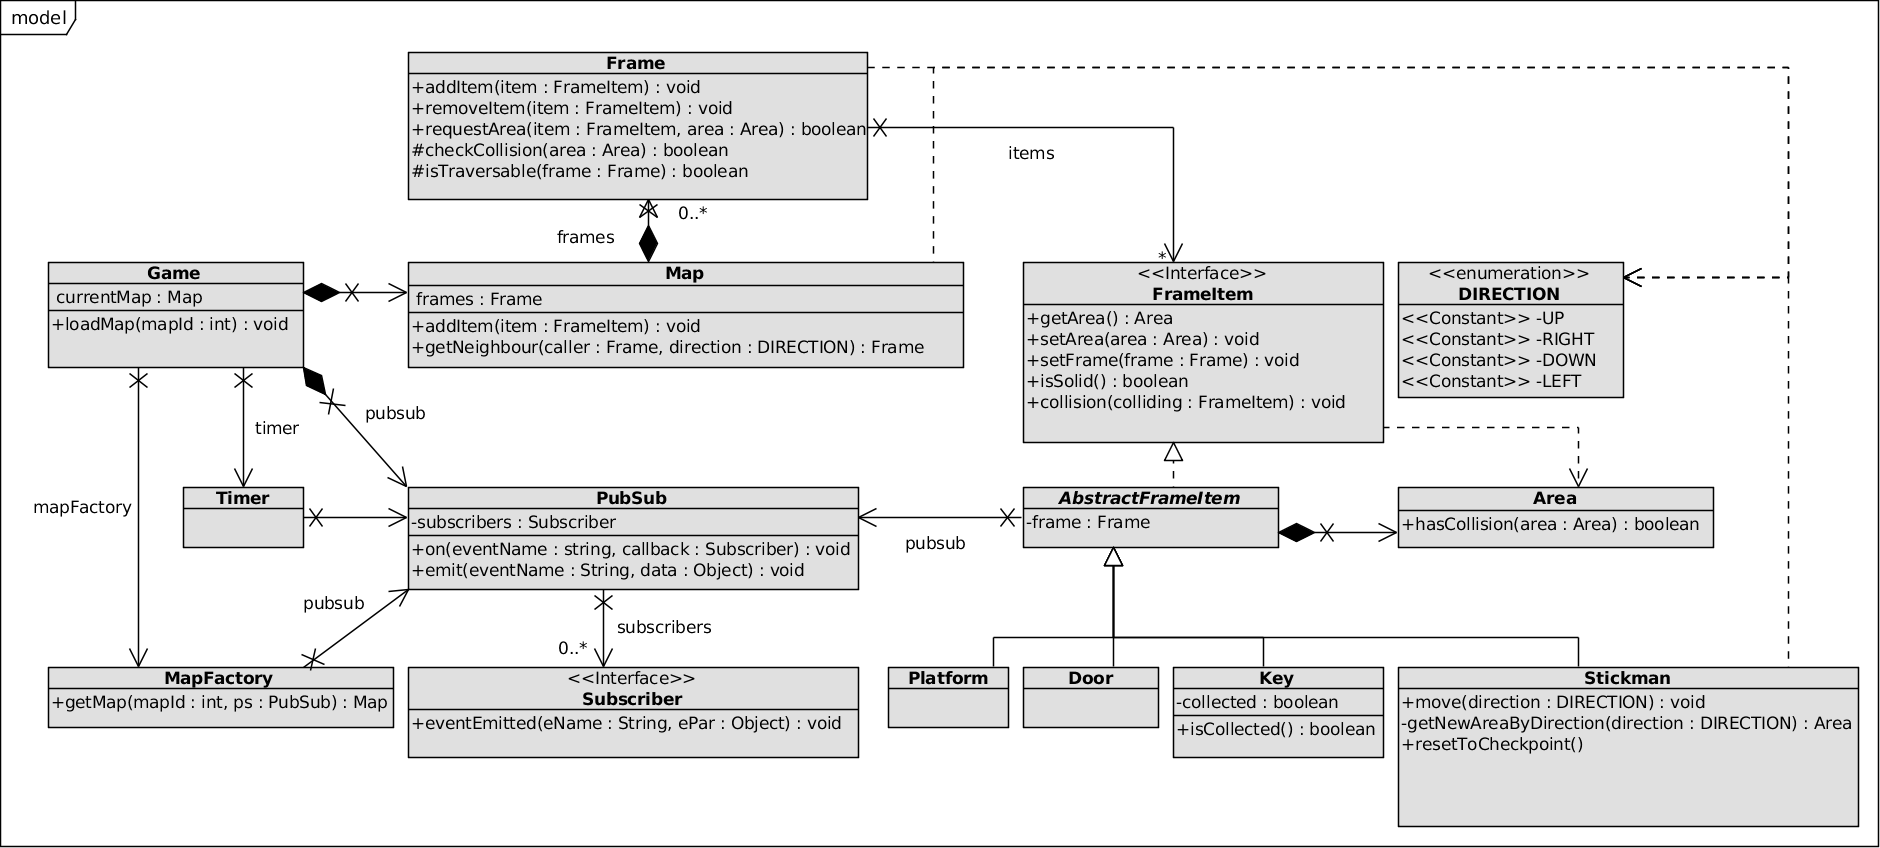
\includegraphics[scale=0.7, angle=-90]{resources/03/model.png}
		\end{center}
			
	\subsection{Szekvencia diagramok}
	
\begin{center}\includegraphics[scale=1]{resources/03/10LoadGame.png}\end{center}
\begin{center}\includegraphics[scale=0.8]{resources/03/12AddFrameItemtoMap.png}\end{center}
\begin{center}\includegraphics[scale=1, angle=-90]{resources/03/11LoadMap.png}\end{center}
\begin{center}\includegraphics[scale=1]{resources/03/20StickmanMoves.png}\end{center}
\begin{center}\includegraphics[scale=0.8, angle=-90]{resources/03/21InterframeMove.png}\end{center}
\begin{center}\includegraphics[scale=1]{resources/03/22FrameChecksCollision.png}\end{center}
\begin{center}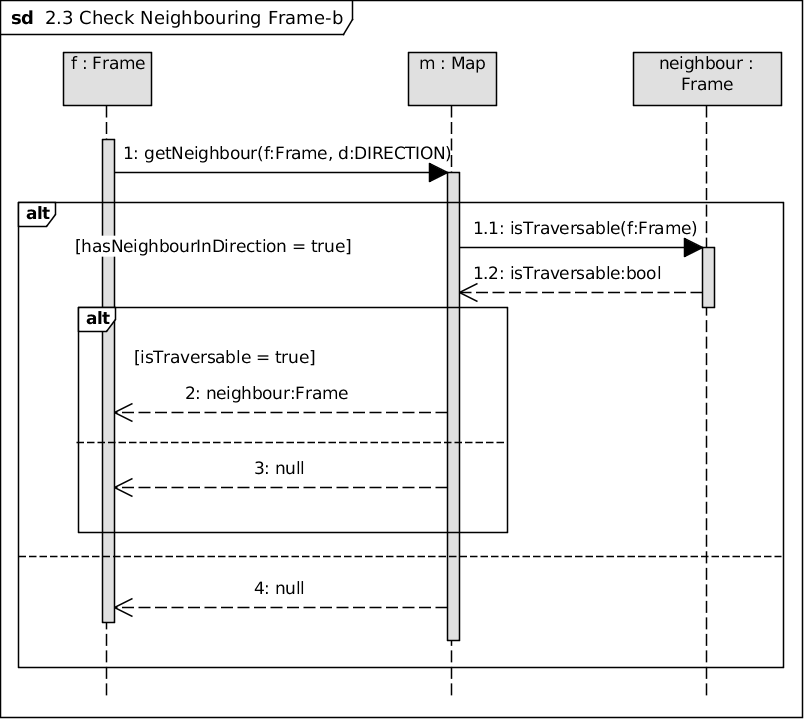
\includegraphics[scale=1]{resources/03/23CheckNeighbouringFrame.png}\end{center}
\begin{center}\includegraphics[scale=1]{resources/03/24Stickmanfalls.png}\end{center}
\begin{center}\includegraphics[scale=1]{resources/03/25Pickingupakey.png}\end{center}
\begin{center}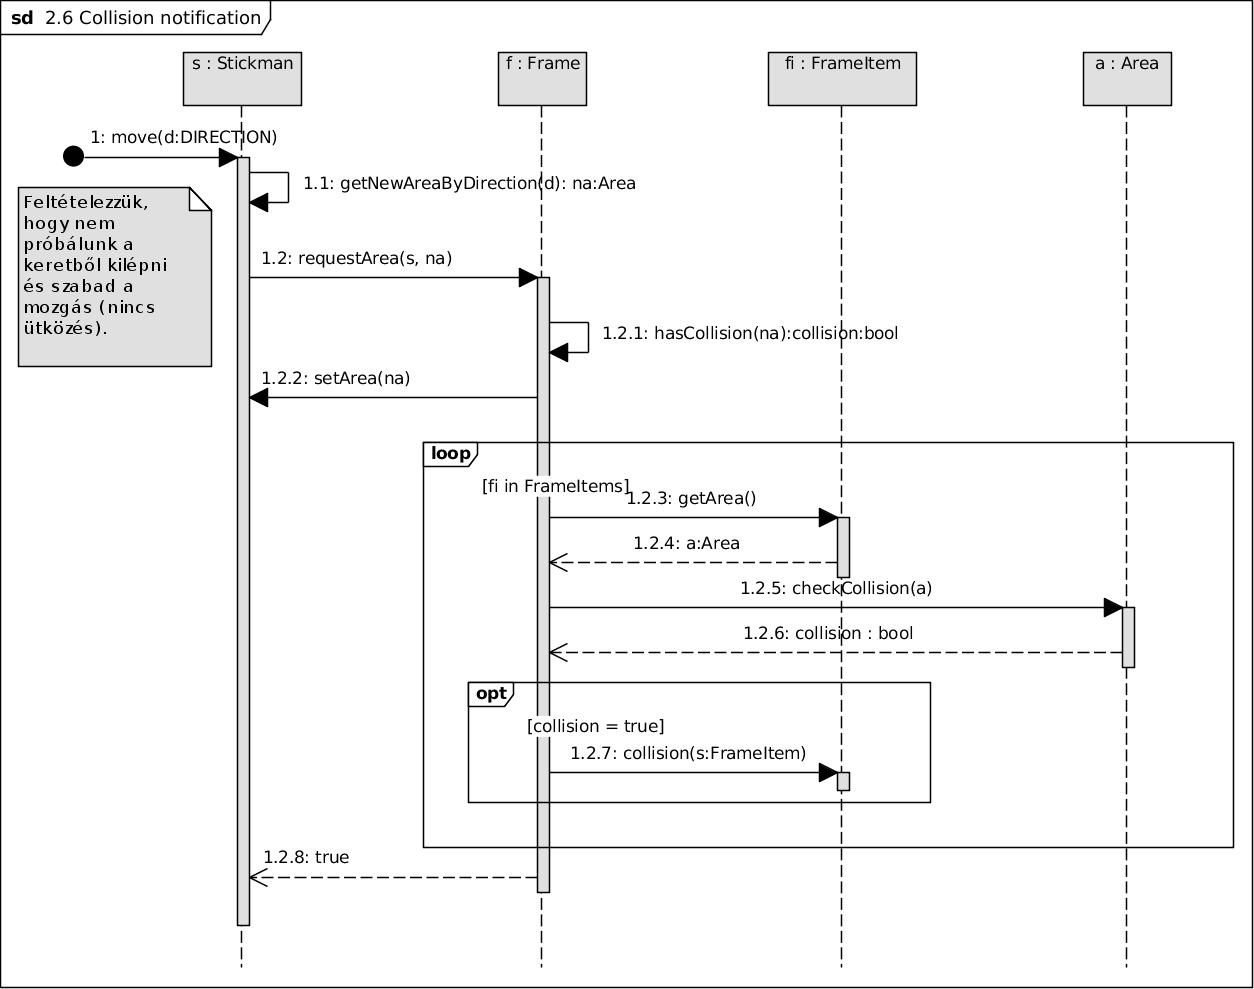
\includegraphics[scale=0.8, angle=-90]{resources/03/26Collisionnotification.png}\end{center}

	\subsection{State-chartok}
\begin{center}\includegraphics[scale=1]{resources/03/10Key.png}\end{center}	
\begin{center}\includegraphics[scale=1]{resources/03/20Viewport.png}\end{center}

	
	\subsection{Napló}
	% The diary generator uses the following comments to identify the beginning and the ending of the generated diary
	% The following content is auto generated, please do NOT modify, edit the related shared document instead.
	%GENERATOR:DIARY
    \begin{center} 
        \begin{tabular}{| l | p{1.9cm} | p{2.6cm} | p{6.1cm} |}
            \hline
                Kezdet & Időtartam & Résztvevők & Leírás \\
            \hline \hline 
2012. 02. 21. 20:00 & 1 óra & Fodor & Visual Paradigm modellező eszköz lehetőségeinek felmérése\\ \hline
2012. 02. 22. 12:00 & 0.5 óra & Értekezlet & Második fázis feladatainak megbeszélése. Döntés: Thaler közzéteszi a munkák alapját adó UML diagramot\\ \hline
2012. 02. 22. 18:30 & 1.5 óra & Thaler & 03. latex gerinc, korábbi hibák javítása\\ \hline
2012. 02. 22. 20:00 & 0.5 óra & Thaler & *.vpp fájlok verziókezelési lehetőségeinek vizsgálata\\ \hline
2012. 02. 22. 20:00 & 1.5 óra & Fodor & Eclipse - VP integráció vizsgálata\\ \hline
2012. 02. 22. 20:30 & 2 óra & Thaler & Class és Szekv. diagramok készítése\\ \hline
2012. 02. 22. 8:00 & 1.5 óra & Fodor, Kádár, Thaler & Konzultáció\\ \hline
2012. 02. 23. 15:30 & 3 óra & Kádár & Java kód generálás, dokumentálás\\ \hline
2012. 02. 23. 19:00 & 1.5 óra & Thaler & Sequence diagramok készítése\\ \hline
2012. 02. 23. 20:00 & 2 óra & Fodor & Modellezés\\ \hline
2012. 02. 25. 15:00 & 3 óra & Thaler & Sequence diagramok készítése\\ \hline
2012. 02. 26. 08:00 & 1.5 óra & Kádár & Beadandó dokumentum átnézése, nyomtatása\\ \hline
2012. 02. 26. 11:00 & 1 óra & Thaler & Sequence diagramok készítése\\ \hline
2012. 02. 26. 13:30 & 1.5 óra & Thaler & Class diagram készítése\\ \hline
2012. 02. 26. 15:00 & 2.5 óra & Thaler & JavaToLatex tool szerkesztése\\ \hline
2012. 02. 26. 17:30 & 1.5 óra & Thaler & Osztályok dokumentálása\\ \hline
2012. 02. 26. 18:00 & 7 óra & Fodor & Modellezés, Diagramok átnézése/kiegészítése, felelősségek dokumentálása\\ \hline
2012. 02. 26. 19:30 & 2 óra & Thaler & Modellezés\\ \hline
2012. 02. 26. 20:00 & 1 óra & Berki & UML -> PNG transzformáció és latex beillesztés\\ \hline
2012. 02. 26. 21:30 & 1 óra & Thaler & javaToLatex tool autoinsert\\ \hline
2012. 02. 26. 22:20 & 3 óra & Kádár & UML to vektorformátum\\ \hline
2012. 02. 26. 22:30 & 2.5 óra & Thaler & Generált tartalmak beillesztése, tisztítás, napló\\ \hline

            \hline
        \end{tabular}
    \end{center}
%GENERATOR:DIARY

\newpage
\section{Analízis modell kidolgozása}

	\subsection{Objektum katalógus}
%GENERATOR:CLASS_RESPONSIBILITY
		\begin{description}
			\item[AbstractFrameItem] Alapértelmezett megvalósítása egy keretben lévő objektumnak.
			\item[Area] Területrészt leíró osztály. Összehasonlítható egy másik osztállyal, hogy fedik-e egymást.
			\item[DIRECTION] Irányokat jelöl a két dimenziós térben.
			\item[Door] Ajtó objektum, melyet ha megérint a Stickman arról esemény bocsát ki.
			\item[Frame] A pálya által alkotott táblázat egy cellája, amely elemeket tartalmaz. Ez felelős az elemek (Stickman) mozgatásáért kereten belül és között egyaránt. Két elem egy helyen való tartózkodásáról értesíti az elemeket (collision notify).
			\item[FrameItem] A keretben elhelyezkedő elemek által megvalósított iterfész, melyen keresztül a keret menedzselni tudja a benne lévő elemeket.
			\item[Game] A játékot reprezentáló objektum, amely kezeli az aktuális pályát.
			\item[Key] Kulcs elem, melyet megérintve a Stickman meg tud szerezni. Erről egy esemény küldésén keresztül értesíti a külvilágot.
			\item[Map] Számon tartja a pályán elhelyezett kulcsokat számát, valamint a már összegyűjtött kulcsok számát. Felelős a keretek mozgatásáért, amit kommunikácó nélkül meg tud valósítani.
			\item[MapFactory] Felelős a pályák létrehozásáért, bennük a keretek és az elemek elhelyezéséért.
			\item[Platform] Olyan elem, mellyel nem tud a Stickman egy helyen tartózkodni, azaz korlátozza a Stickman mozgásterét.
			\item[PubSub] Üzenetközvetítő osztály, mely feliratkozásokat tart számon, és ha valakitől eseményt kap, arról értesíti az arra feliratkozottakat.
			\item[Stickman] A játékos által irányított figura, mely a pályán mozog.
			\item[Subscriber] Olyan interfész, melyen keresztül eseményeket lehet fogadni a PubSubtól.
			\item[Timer] Időzítésért felelős osztály, bizonyos időközönként kibocsát egy 'tick' eseményt az átadott PubSub objektumra.
		\end{description}
%GENERATOR:CLASS_RESPONSIBILITY	
	
	\subsection{Osztályok leírása}
	
%GENERATOR:CLASS_DESCRIPTIONS
		\subsubsection{AbstractFrameItem} Absztrakt osztály.
				 Alapértelmezett megvalósítása egy keretbe helyezett objektumnak.   Nyilvántartja a kereten belüli pozícióját, valamint hordoz  egy referenciát a tartalmazó keretre. 			\begin{description}


				\item[Ősosztályok] (nincs).
				\item[Interfészek] FrameItem.
				\item[Attribútumok]$\ $
					\begin{description}
						\item[\texttt{protected Area area}] A tartalmazó kereten belül elfoglalt pozíció 
						\item[\texttt{protected Frame frame}] A tartalmazó keret 
					\end{description}
				\item[Metódusok] (nincs)
			\end{description}

		\subsubsection{Area}
				 Egy tetszőleges keret egy területét leíró osztály.  Ez az osztály elfedi, hogy egy keret valójában hány dimenziós,  valamint azt, hogy egy keret egy összefüggő ponthalmaza milyen   paraméterekkel írható le. 			\begin{description}


				\item[Ősosztályok] (nincs).
				\item[Interfészek] (nincs)
				\item[Attribútumok]$\ $
					\begin{description}
						\item[\texttt{private int height}] A terület magassága 
						\item[\texttt{private int width}] A terület szélessége 
						\item[\texttt{private int x}] A terület bal felső sarkának x eltolása 
						\item[\texttt{private int y}] A terület bal felső sarkának y eltolása 
					\end{description}
				\item[Metódusok]$\ $
					\begin{description}
%						\item[\texttt{public int getHeight()}] \hfill \\
						% TODO document getHeight
%						\item[\texttt{public int getWidth()}] \hfill \\
						% TODO document getWidth
%						\item[\texttt{public int getX()}] \hfill \\
						% TODO document getX
%						\item[\texttt{public int getY()}] \hfill \\
						% TODO document getY
						\item[\texttt{public boolean hasCollision(Area area)}] \hfill \\ Ellenőrzi, hogy a kapott Area objektummal van-e közös pontja.  A metódus feltételezi, hogy a két terület azonos keretben található. 
%						\item[\texttt{public void setHeight(int height)}] \hfill \\
						% TODO document setHeight
%						\item[\texttt{public void setWidth(int width)}] \hfill \\
						% TODO document setWidth
%						\item[\texttt{public void setX(int x)}] \hfill \\
						% TODO document setX
%						\item[\texttt{public void setY(int y)}] \hfill \\
						% TODO document setY
					\end{description}
			\end{description}

		\subsubsection{DIRECTION}
				 Enumeráció. Elfedi, hogy a játéktér hány dimenziós.  A tartalmazott elemek leírják az összes lehetséges irányt,   melybe a játékos mozoghat, vagy keretet cserélhet.  			\begin{description}


				\item[Ősosztályok] (nincs).
				\item[Interfészek] (nincs)
				\item[Attribútumok] (nincs)
				\item[Metódusok] (nincs)
			\end{description}

		\subsubsection{Door}
				 A pályák befejezésére szolgáló ajtót reprezentálja.  Ha a Stickman az összes kulcs birtokában megérinti,  a pálya teljesítésre kerül. 			\begin{description}


				\item[Ősosztályok] AbstractFrameItem $\rightarrow{}$ Door.
				\item[Interfészek] (nincs)
				\item[Attribútumok] (nincs)
				\item[Metódusok] (nincs)
			\end{description}

		\subsubsection{Frame}
				 Egy pályán belüli keret, amelyben mozoghat a Stickman. Tartalmazza a pálya többi elemét (Door, Key, Platform). 			\begin{description}


				\item[Ősosztályok] (nincs).
				\item[Interfészek] (nincs)
				\item[Attribútumok] (nincs)
				\item[Metódusok]$\ $
					\begin{description}
						\item[\texttt{public void addItem(FrameItem item)}] \hfill \\ Hozzáadja a megadott elemet a kerethez. 
						\item[\texttt{protected boolean checkCollision(Area area)}] \hfill \\ Ellenőrzi, hogy a megadott területen  található-e szilárd objektum. 
						\item[\texttt{protected boolean isTraversable(Frame frame, DIRECTION d)}] \hfill \\ Megállapítja, hogy a megkapott Keret és saját  maga között fennáll-e az átjárhatóság a  megadott irányban. 
						\item[\texttt{public void removeItem(FrameItem item)}] \hfill \\ Eltávolítja a megadott elemet a keretből 
						\item[\texttt{public boolean requestArea(FrameItem item, Area area)}] \hfill \\ A metódust hívó elem kérést intéz a kerethez,  hogy el szeretné foglalni a megadott területet.  A keret felelőssége a terület ellenőrzése, és szabad  terület esetén az elem pozíciójának frissítése. 
					\end{description}
			\end{description}

		\subsubsection{FrameItem} Interfész.
				 A Frame osztály ezen a felületen keresztül éri el a tartalmazott objektumokat.   Ezen interfacet valósítják meg a pályán lévő objektumok (Platform, Door, Key, Stickman) 			\begin{description}


				\item[Ősosztályok] (nincs).
				\item[Metódusok]$\ $
					\begin{description}
						\item[\texttt{public void collision(FrameItem colliding)}] \hfill \\ A tartalmazó keret jelezheti ezen a metóduson keresztül,  hogy egy másik elem, melyet paraméterül ad,  hozzáért (collision) ehez az elemhez. 
						\item[\texttt{public Area getArea()}] \hfill \\ Visszaadja az elem pozícióját a kereten belül. 
						\item[\texttt{public boolean isSolid()}] \hfill \\ Megadja, hogy az elem szilárd-e vagy sem.  Ez a kereten belüli mozgások esetén az  ütközések ellenőrzésekor használatos. 
						\item[\texttt{public void setArea(Area area)}] \hfill \\ Beállítja az elem pozícióját a kereten belül. 
						\item[\texttt{public void setFrame(Frame frame)}] \hfill \\ Beállítja az elemet tartalmazó keretet. 
					\end{description}
			\end{description}

		\subsubsection{Game}
				 A játékot szervező objektum. Felelős az új pályák betöltéséért és a teljesített pályák törléséért. 			\begin{description}


				\item[Ősosztályok] (nincs).
				\item[Interfészek] (nincs)
				\item[Attribútumok]$\ $
					\begin{description}
						\item[\texttt{protected Map currentMap}] Az aktuális pálya 
					\end{description}
				\item[Metódusok]$\ $
					\begin{description}
						\item[\texttt{public void loadMap(int mapId)}] \hfill \\ Betölti a megadott pályát. 
					\end{description}
			\end{description}

		\subsubsection{Key}
				 A pályán található kulcsokat reprezentáló objektum. 			\begin{description}


				\item[Ősosztályok] AbstractFrameItem $\rightarrow{}$ Key.
				\item[Interfészek] (nincs)
				\item[Attribútumok]$\ $
					\begin{description}
						\item[\texttt{private boolean collected}] A kulcs összegyűjtöttségének állapotát tárolja. 
					\end{description}
				\item[Metódusok]$\ $
					\begin{description}
						\item[\texttt{public boolean isCollected()}] \hfill \\ Megadja, hogy megszerezték-e a kulcsot. 
					\end{description}
			\end{description}

		\subsubsection{Map}
				 A pályákat reprezentálja. Tartalmazza a kereteket és azok elhelyezkedését,  kontrolállja az átrendezésüket, melyet kommunikáció nélkül meg tud tenni, mivel a keretek nem tudnak relatív elhelyezkedésükről. 			\begin{description}


				\item[Ősosztályok] (nincs).
				\item[Interfészek] (nincs)
				\item[Attribútumok]$\ $
					\begin{description}
						\item[\texttt{protected Collection<Frame> frames}] A pályához tartozó kereteket tárolja. A Map osztály  meg tudja állapítani a keretek közötti szomszédossági  viszonyokat a gyűjtemény alapján. 
					\end{description}
				\item[Metódusok]$\ $
					\begin{description}
						\item[\texttt{public void addItem(FrameItem item)}] \hfill \\ Hozzáadja a megadott elemet az elem által specifikált pozícióhoz.  Amennyiben a pálya inicializálása során az adott helyen még nincs keret,  létrehoz egyet.   A hozzáadott elem pozícióját megváltoztatja úgy, hogy az relatív  legyen a tartalmazó kerethez. 
						\item[\texttt{public Frame getNeighbour(Frame caller, DIRECTION direction)}] \hfill \\ Visszaadja a megadott keret direction irányba található  szomszédját. null-t ad vissza, ha a megadott irányban  nincs szomszéd. 
						\item[\texttt{public void moveFrame(DIRECTION d)}] \hfill \\ Kicseréli az üres helyet a megadott iránnyal ellentétes  szomszédjával. 
					\end{description}
			\end{description}

		\subsubsection{MapFactory}
				 Azonosító alapján Pályákat szolgáltat.  Létrehozza a pályát, majd az azonosító alapján feltölti  a megfelelő objektumokkal. 			\begin{description}


				\item[Ősosztályok] (nincs).
				\item[Interfészek] (nincs)
				\item[Attribútumok] (nincs)
				\item[Metódusok]$\ $
					\begin{description}
						\item[\texttt{public Map getMap(int mapId, PubSub ps)}] \hfill \\ Létrehozza a megadott azonosítójú pályát  és feltölti elemekkel. 
					\end{description}
			\end{description}

		\subsubsection{Platform}
				 A Stickman és ezzel a játék mozgásterét korlátozó elem. A framen belül bejárható rész keretezésére szolgál. 			\begin{description}


				\item[Ősosztályok] AbstractFrameItem $\rightarrow{}$ Platform.
				\item[Interfészek] (nincs)
				\item[Attribútumok] (nincs)
				\item[Metódusok] (nincs)
			\end{description}

		\subsubsection{PubSub}
				 Üzenetközvetítő csatorna, mely a Publish/Subscribe mintát valósítja meg. 			\begin{description}


				\item[Ősosztályok] (nincs).
				\item[Interfészek] (nincs)
				\item[Attribútumok]$\ $
					\begin{description}
						\item[\texttt{private Collection<Subscriber> subscribers}] Az eseményekre feliratkozott eseménykezelőket tárolja. 
					\end{description}
				\item[Metódusok]$\ $
					\begin{description}
						\item[\texttt{public void emit(String eventName, Object data)}] \hfill \\ Esemény publikálása 
						\item[\texttt{public void on(String eventName, Subscriber callback)}] \hfill \\ Feliratkozás eseményre 
					\end{description}
			\end{description}

		\subsubsection{Stickman}
				 A játékos által irányított figurát reprezentáló elem. 			\begin{description}


				\item[Ősosztályok] AbstractFrameItem $\rightarrow{}$ Stickman.
				\item[Interfészek] (nincs)
				\item[Attribútumok] (nincs)
				\item[Metódusok]$\ $
					\begin{description}
						\item[\texttt{private Area getNewAreaByDirection(DIRECTION direction)}] \hfill \\ A figura igényelt elmozdulása után elfoglalandó  terület kiszámítása. 
						\item[\texttt{public void move(DIRECTION direction)}] \hfill \\ A figura mozgatása a megadott irányba. 
						\item[\texttt{public void resetToCheckpoint()}] \hfill \\ A figura pozíciójának visszaállítása az  utolsó ellenőrzőpontra. 
					\end{description}
			\end{description}

		\subsubsection{Subscriber} Interfész.
				 A PubSub objektumnak átadható eseménykezelő felülete. 			\begin{description}


				\item[Ősosztályok] (nincs).
				\item[Metódusok]$\ $
					\begin{description}
						\item[\texttt{public void eventEmitted(String eName, Object eParameter)}] \hfill \\ A PubSub objektum által meghívott metódus,  a feliratkozott esemény bekövetkeztekor. 
					\end{description}
			\end{description}

		\subsubsection{Timer}
				 Az idő múlását nyilvántartó objektum.   Elsősorban Stickman esését szabályozhatjuk vele, de a  periodikus időközönként kiadott 'tick' események  a stickmentől vagy bármely más objektumtól függetlenek.  			\begin{description}


				\item[Ősosztályok] (nincs).
				\item[Interfészek] (nincs)
				\item[Attribútumok]$\ $
					\begin{description}
						\item[\texttt{ PubSub pubsub}] Az eseménykezelő csatorna,  melyen jelzi az idő múlását. 
					\end{description}
				\item[Metódusok] (nincs)
			\end{description}

%GENERATOR:CLASS_DESCRIPTIONS

	\subsection{Statikus struktúra diagramok}

		\begin{center}
			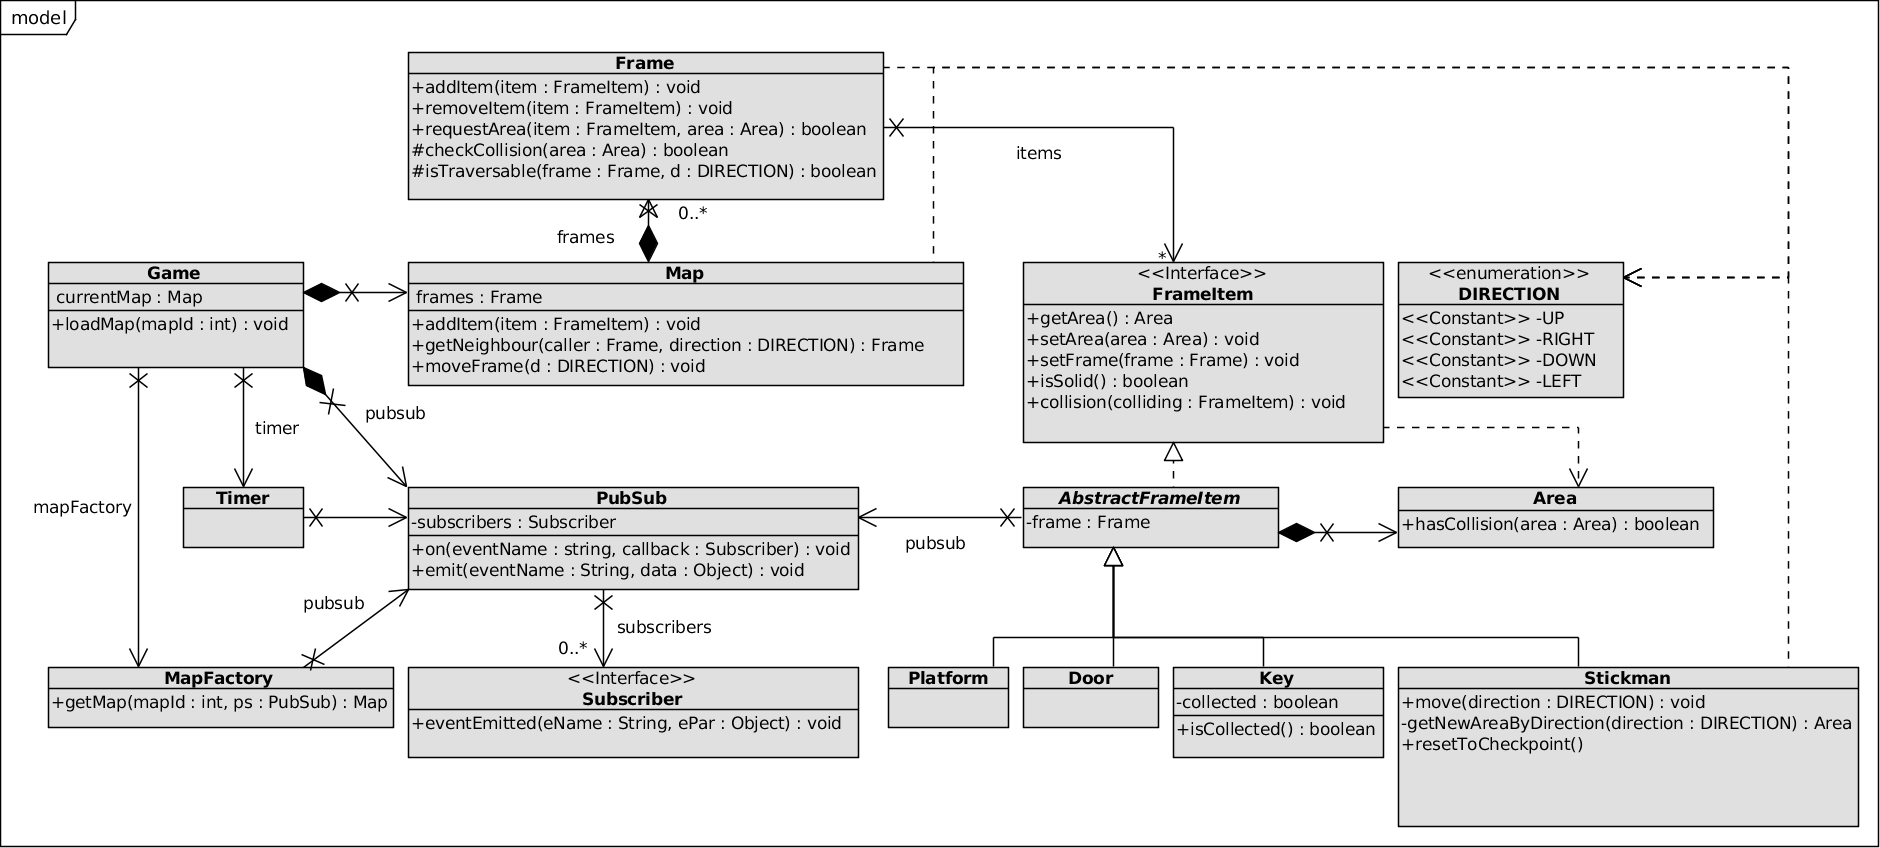
\includegraphics[scale=0.7, angle=-90]{resources/04/model.png}
		\end{center}
			
	\subsection{Szekvencia diagramok}
	
\begin{center}\includegraphics[scale=1]{resources/04/10LoadGame.png}\end{center}
\begin{center}\includegraphics[scale=0.8]{resources/04/12AddFrameItemtoMap.png}\end{center}
\begin{center}\includegraphics[scale=1, angle=-90]{resources/04/11LoadMap.png}\end{center}
\begin{center}\includegraphics[scale=1]{resources/04/20StickmanMoves.png}\end{center}
\begin{center}\includegraphics[scale=0.8, angle=-90]{resources/04/21InterframeMove.png}\end{center}
\begin{center}\includegraphics[scale=1]{resources/04/22FrameChecksCollision.png}\end{center}
\begin{center}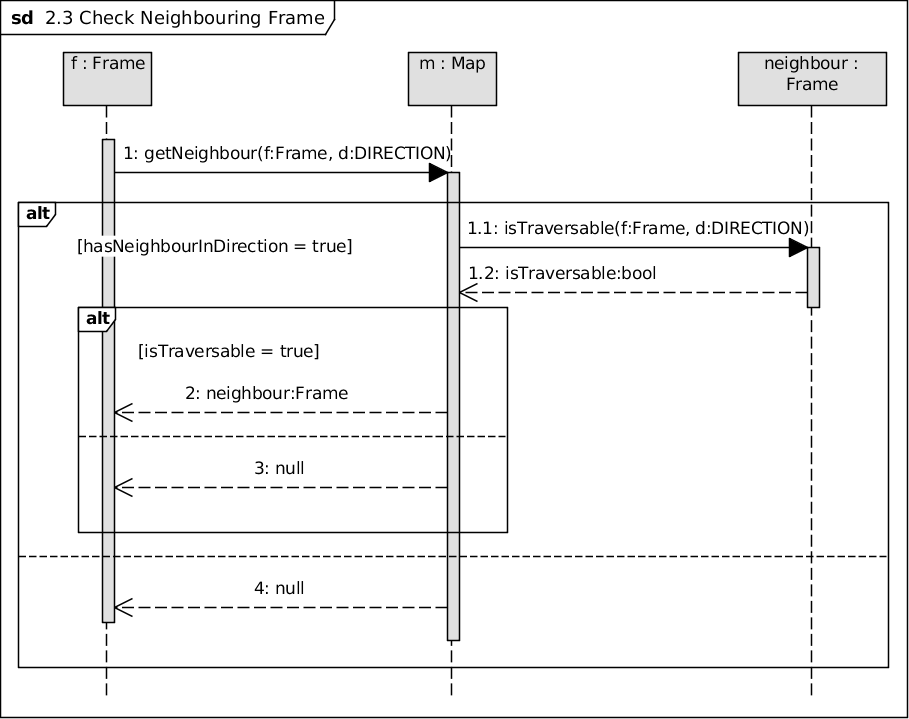
\includegraphics[scale=1]{resources/04/23CheckNeighbouringFrame.png}\end{center}
\begin{center}\includegraphics[scale=1]{resources/04/24Stickmanfalls.png}\end{center}
\begin{center}\includegraphics[scale=1]{resources/04/25Pickingupakey.png}\end{center}
\begin{center}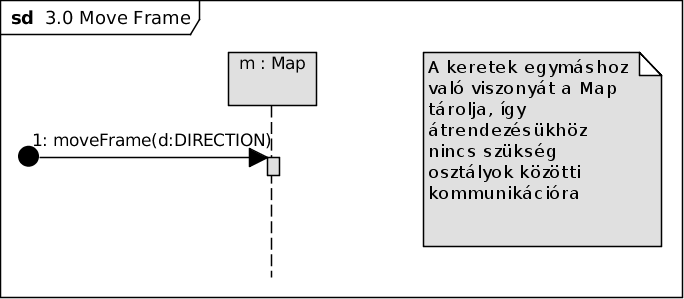
\includegraphics[scale=1]{resources/04/30MoveFrame.png}\end{center}
\begin{center}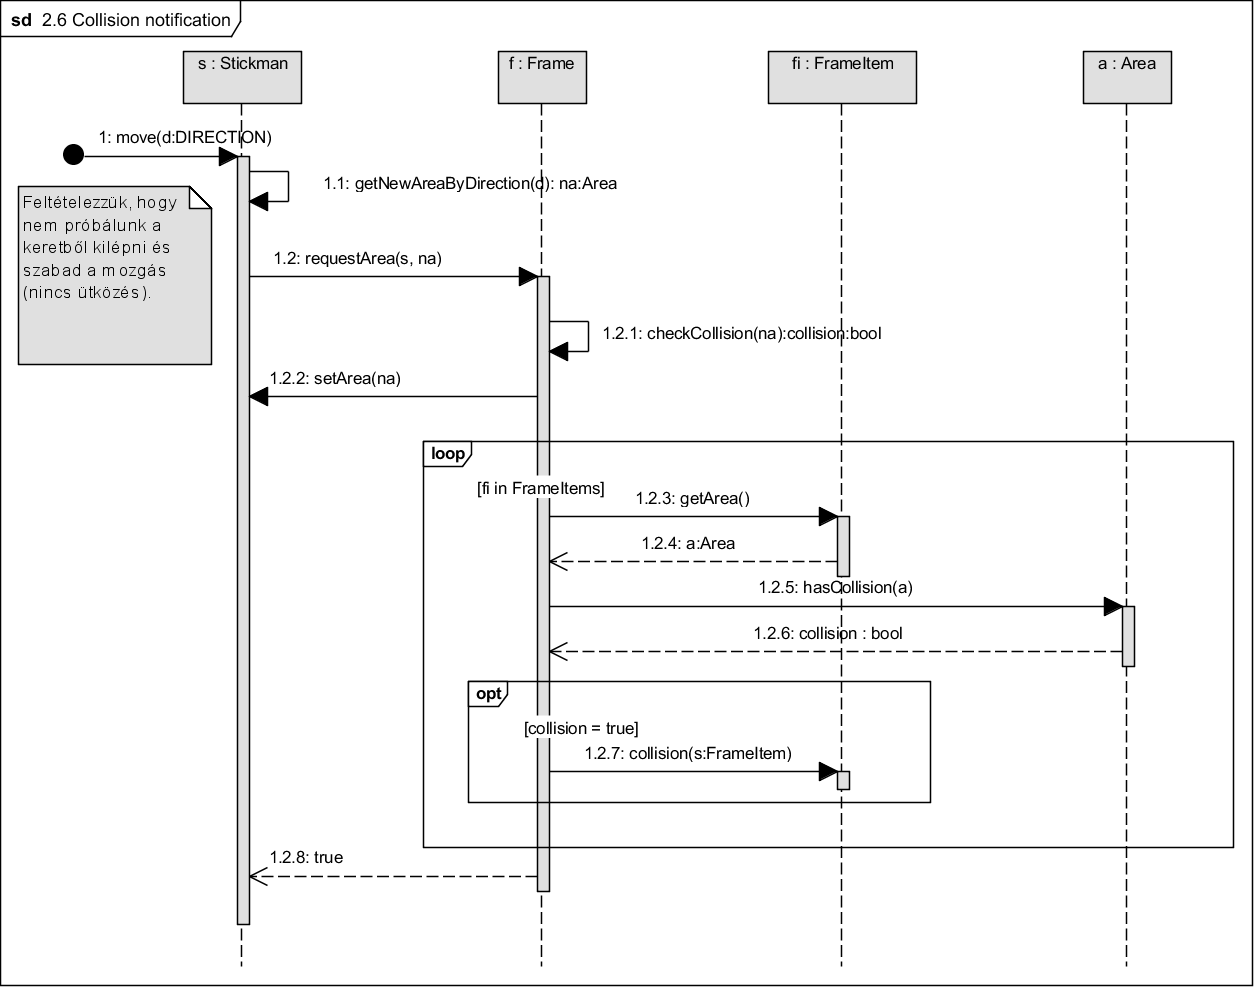
\includegraphics[scale=0.8, angle=-90]{resources/04/26Collisionnotification.png}\end{center}

	\subsection{State-chartok}
\begin{center}\includegraphics[scale=1]{resources/04/10Key.png}\end{center}	
\begin{center}\includegraphics[scale=1]{resources/04/20Viewport.png}\end{center}

	
	\subsection{Napló}
	% The diary generator uses the following comments to identify the beginning and the ending of the generated diary
	% The following content is auto generated, please do NOT modify, edit the related shared document instead.
	%GENERATOR:DIARY
    \begin{center} 
        \begin{tabular}{| l | p{1.9cm} | p{2.6cm} | p{6.1cm} |}
            \hline
                Kezdet & Időtartam & Résztvevők & Leírás \\
            \hline \hline 
2012. 02. 29. 08:00 & 1.5 óra & Fodor, Thaler & Konzultáció\\ \hline
2012. 02. 29. 16:30 & 1.5 óra & Thaler & Kért módosítások implementálása\\ \hline
2012. 02. 30. 21:00 & 3 óra & Berki & Javítások átnézése\\ \hline
2012. 02. 31. 19:00 & 2 óra & Berki & További javítások\\ \hline
2012. 03. 04. 20:00 & 1.5 óra & Thaler & Sequence diagram javítás\\ \hline
2012. 03. 05. 21:30 & 0.5 óra & Berki & Nyomtatás\\ \hline

            \hline
        \end{tabular}
    \end{center}
%GENERATOR:DIARY

\newpage
\section{Szkeleton tervezése}

	\subsection{A szkeleton modell valóságos use case-ei}
        %domain specific commands
        \newcommand{\ucitem}[1]{\item \textbf{Use case neve: } #1\\}
        \newcommand{\ucdesc}[1]{\textbf{Leírás: } #1\\}
        \newcommand{\ucscenario}[1]{\textbf{Forgatókönyv: }#1\\}
        
		\subsubsection{Játékos use case diagram}
		    \begin{center}
			    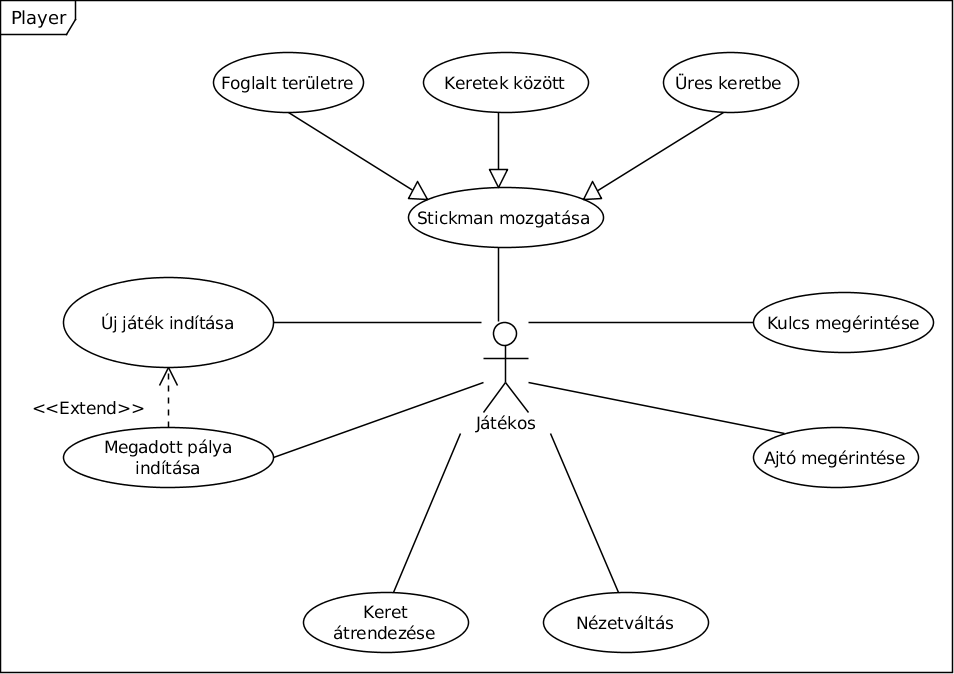
\includegraphics[scale=0.9]{resources/05/Player.png}
		    \end{center}
		
		\subsubsection{Játékos use case leírások}
		    Az alábbi use case leírások mindegyikének esetében az aktor a szkeleton programot kezelő Játékos.
		    
		    \begin{enumerate}[label=\textbf{\arabic*.}, start=1]
                \ucitem{Új játék indítása}
                    \ucdesc{A játékos új játékot indít.}
                    \ucscenario{Az új játék indítása során létrejön a játékot reprezentáló Game objektum, a pályákat előállító MapFactory, az időzítést végző Timer valamint az üzenetküldést segítő PubSub objektum. A Game objektum az inicializálás után betölti a MapFactory segítségével az első pályát.}
                    
                \ucitem{Megadott pálya indítása}
                    \ucdesc{A játékos meghatározza a betöltendő pályát.}
                    \ucscenario{Megegyezik az előzővel, azzal a különbséggel, hogy a Game objektum az első pálya helyett a megadott pályát tölti be.}
                    
                \ucitem{Stickman mozgatása}
                    \ucdesc{A játékos egy megadott irányba mozgatja a stickmant.}
                    \ucscenario{A Stickman objektum előállítja az elfoglalni kívánt Area objektumot, majd kérést intéz a tartalmazó Frame objektumhoz a terület elfoglalására. Amennyiben a terület szabad, az új területhez tartozó Frame beállítja a Stickman új helyét.}
                    
                \ucitem{(Stickman mozgatása) Foglalt területre.}
                    \ucdesc{A játékos olyan irányba szeretné mozgatni a stickmant, amerre Platform található.}
                    \ucscenario{Megegyezik az előzővel, azzal a különbséggel, hogy mivel az igényelt terület foglalt, a tartalmazó keret nem állít be új helyet, és false értékkel tér vissza}
                    
                \ucitem{(Stickman mozgatása) Keretek között}
                    \ucdesc{A játékos a stickmant a kerethatáron keresztül egy másik keretbe mozgatja.}
                    \ucscenario{A Stickman objektum előállítja az elfoglalni kívánt Area objektumot, majd kérést intéz a tartalmazó Frame objektumhoz a terület elfoglalására. Miután a tartalmazó keret meggyőződik arról, hogy a Stickman objektum elhagyja a területét, a Map objektumhoz fordul a szomszédjáért. A két keret közötti átjárhatóság és az új keretben elfoglalandó hely szabad mivolta ellenőrzésre kerül, a régi keret átadja a Stickman objektumot az új keretnek és az új keret állítja be az új pozíciót. Amennyiben az átjárhatóság vagy terület szabadsága nem teljesül, az eredeti keret false értékkel tér vissza, és nem állít be új pozíciót.}
                    
                \ucitem{(Stickman mozgatása) Üres keretbe}
                    \ucdesc{A játékos a stickmant a kerethatáron keresztül az üres keretbe mozgatja.}
                    \ucscenario{A Stickman objektum előállítja az elfoglalni kívánt Area objektumot, majd kérést intéz a tartalmazó Frame objektumhoz a terület elfoglalására. Miután a tartalmazó keret meggyőződik arról, hogy a Stickman objektum elhagyja a területét, a Map objektumhoz fordul a szomszédjáért. Mivel az adott irányban üres keret található, a Map objektum nullal tér vissza. Amennyiben a mozgás iránya lefelé mutat, a stickman kiesik és a keret visszaállítattja az utolsó ellenőrzőpontra. Más esetben false értékkel tér vissza, és nem állít be új pozíciót.}
                    
                \ucitem{Kulcs megérintése}
                    \ucdesc{A stickman mozgás során felvesz egy kulcsot.}
                    \ucscenario{Miután a stickman mozgatása miatt a tartalmazó keret beállította az új helyét, jelzi a kulcs objektumnak, hogy megérintették, amennyiben a stickman új helyének és a kulcs objektum által elfoglalt helynek van közös metszete.}
                    
                \ucitem{Ajtó megérintése}
                    \ucdesc{A stickman mozgás során egy ajtóhoz ér.}
                    \ucscenario{Miután a stickman mozgatása miatt a tartalmazó keret beállította az új helyét, jelzi az ajtó objektumnak, hogy megérintették, amennyiben a stickman új helyének és az ajtó objektum által elfoglalt helynek van közös metszete.}
                    
                \ucitem{Keret átrendezése}
                    \ucdesc{A játékos mozgat egy keretet.}
                    \ucscenario{A játékos megadja a mozgatás irányát. A Map objektum, mely a kereteket tartalmazza, megkeresi az üres keretet. Amennyiben a megadott iránnyal ellenkező irányban van szomszédja az üres keretnek, kicseréli a kettőt, ellenkező esetben tétlen. A keretek átrendezése nem igényel objektumok közötti kommunikációt, azt a Map objektum önmagában el tudja végezni.}
                    
                \ucitem{Nézetváltás}
                    \ucdesc{A játékos vált pálya és közeli nézet között.}
                    \ucscenario{Felhasználói interakció hatására a Game objektum állapota megváltozik, váltás történik pálya és közeli nézet között. Az állapotváltozás kommunikációt nem igényel, de befolyásolja a Timer actor egyes use case-eit.}
                    
		    \end{enumerate}
		    
		\subsubsection{Óra use case diagram}
		    \begin{center}
			    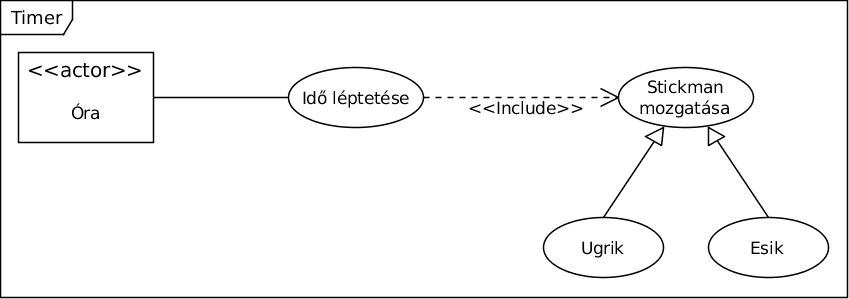
\includegraphics[scale=1]{resources/05/Timer.png}
		    \end{center}
		
		\subsubsection{Óra use case leírások}
		    Az alábbi use case leírások mindegyikének esetében az aktor az idő múlását követő óra (Timer).
		    
		    \begin{enumerate}[label=\textbf{\arabic*.}, start=1]
                \ucitem{Idő léptetése}
                    \ucdesc{A Timer objektum jelzi az idő múlását.}
                    \ucscenario{A Timer objektum előre meghatározott időközönként egy \texttt{tick} eseményt tesz közzé a megadott PubSub objektumon keresztül. Az időre érzékeny objektumok feliratkozhatnak erre az eseményre.}
                    
                \ucitem{Stickman mozgatása}
                    \ucdesc{Az idő múlásával a stickman közvetlen felhasználói interakció nélkül is mozoghat.}
                    \ucscenario{A Stickman objektum a \texttt{tick} esemény hatására -- mely az idő múlását jelzi -- felfelé mozoghat, amennyiben éppen ugrik, ellenkező esetben lefelé mozog (álló helyzetben is esik, mintha hatna rá a gravitációs gyorsulás).}
                    
                \ucitem{(Stickman mozgatása) Ugrik}
                    \ucdesc{Az idő múlásával a stickman egy folyamatos ugrást hajt végre.}
                    \ucscenario{A Stickman objektum a \texttt{tick} esemény hatására -- mely az idő múlását jelzi -- felfelé mozdul, vagyis ugrik. A felfelé történő mozgások száma egy előre meghatározott véges szám. A hátralévő ugrások száma minden egyes felfelé irányuló mozgással csökken.}
                    
                \ucitem{(Stickman mozgatása) Esik}
                    \ucdesc{Az idő múlásával a stickman folyamatosan esik.}
                    \ucscenario{A stickmanre minden pillanatban -- amikor nem ugrik -- lefele irányúló erő hat, ezért a \texttt{tick} esemény hatására -- amikor nincs alatta talaj -- lefelé mozdul (valójában folyamatosan lefelé mozdulna a talajon állva, de ezt a platform megakadályozza).}
		    \end{enumerate}
	
	\subsection{Architektúra}
		A szkeleton architektúrális felépítésének célja, hogy minden egyes use case tesztelhető legyen, valamint meg lehessen állapítani, hogy az előző -- analízisben rögzített -- szekvencia diagramoknak megfelelően működik-e az osztályok közötti kommunikáció. A tesztesetek futtatására előre inicializált pályák állnak majd rendelkezésünkre, hogy a fontos szituációk élesben is tesztelhetőek legyenek. A szkeleton tesztelése szekvenciálisan fog lefutni, ezért nincs szükség a konkurrens feladatok vizsgálatára.
		
		A tesztesetek úgy lettek megválasztva, hogy az adott használati eseteket legjobban mutassák be, minél kevesebb objektummal, hogy a vizsgálandó rész legyen a középpontban. A tesztesetek mellett feltüntettük az általuk használt frame-ek számát, a realizált objektumokat, illetve a tesztelés célját.
		
		Az alábbi tesztesetek az átláthatóság érdekében azon, az 5.1.2. és 5.1.4. use case leírásokban számozott használati esetek számát jelölik, amelyeket megvalósítanak (pl.: P1 -- 1. Játékos use case; T5 -- 5. Timer use case). A csillaggal jelölt use case-ek nagyon hasonlóak a teszteset által kijelölt fő use case-hez, ezért nem igényelnek külön tesztesetet.
								
		\begin{enumerate}[label=\textbf{\arabic*.}, start=0]
		
			\newcommand{\testitem}[1]{\item \textbf{Teszteset -- #1}\\}
			\newcommand{\tframe}[1]{\textbf{Frame-ek száma:} #1\\}
			\newcommand{\tobjekt}[1]{\textbf{Objektumok:} #1\\}
			\newcommand{\tcel}[1]{\textbf{Cél:} #1\\}
			\newcommand{\tuse}[1]{\textbf{Tesztelt use case:} #1\\}
		
			\testitem{Inicializálás}
				\tframe{1}
				\tobjekt{Minden, a futtatáshoz szükséges objektumtípusból legalább egy.
					(Game, Timer, PubSub, MapFactory, Map, Frame, Platform, Door, Key, Stickman stb.)}
				\tcel{Objektumok létrehozása, kapcsolatok kialakításának bemutatása.}
				\tuse{P1, *P2}
			\testitem{Stickman mozgatása}
				\tframe{1}
				\tobjekt{Frame, Stickman, Area, Timer}
				\tcel{A játékos mozdulni szeretne. Bemutatásra kerül a mozgás kérése és az arra kapott válasz, majd léptetés.} 
				\tuse{P3, *T2, *T1}
			\testitem{Stickman ugrása}
				\tframe{1}
				\tobjekt{Frame, Stickman, Timer}
				\tcel{A játékos ugrik, majd leesik, nincs akadály. Idő által kiváltott metódushívások figyelhetőek meg.} 
				\tuse{T3, *T1}
			\testitem{Stickman mozgatása foglalt területre}
				\tframe{1}
				\tobjekt{Frame, Stickman, Platform, Area}
				\tcel{A játékos mozdulni szeretne, de platform állja el az útját. Előzőhöz hasonlóan bemutatható a kommunikáció, kivéve hogy a mozgás kérésre nem kap engedélyt, pozíciója nem fog változni.}
				\tuse{P4}
			\testitem{Stickman mozgatása keretek között}
				\tframe{2}
				\tobjekt{Map, 2 db. Frame, Stickman, Area}
				\tcel{Játékos mozdulni szeretne a jelenlegi keretet elhagyva. Az előzőekhez hasonlóan a kommunikáció bemutatható a Stickman -- Frame, illetve itt a Frame -- Map objektumok között.}
				\tuse{P5}
			\testitem{Stickman mozgatása üres keretbe horizontálisan}
				\tframe{2}
				\tobjekt{Map, 2 db. Frame, Stickman, Area}
				\tcel{Stickman -- Frame, Frame -- Map kommunikáció bemutatása, lépés megtagadásával (nincs Frame).}
				\tuse{P6}
			\testitem{Stickman kiesése keretből}
				\tframe{2}
				\tobjekt{Map, 2 db. Frame, Stickman, Area, Timer}
				\tcel{Stickman -- Frame, Frame -- Map kommunikáció bemutatása, utolsó ellenőrzőpontra visszaállítás.}
				\tuse{P6, *T4, *T1}
			\testitem{Kulcs felvétele}
				\tframe{1}
				\tobjekt{PubSub, Frame, Stickman, Key, Area}
				\tcel{A játékos kulcsot tartalmazó mezőbe lép, kulcs felvétele. Üzenet terjedésének bemutatása.}
				\tuse{P7}
			\testitem{Ajtó megérintése}
				\tframe{1}
				\tobjekt{PubSub, Frame, Stickman, Door, Area}
				\tcel{A játékos az ajtót tartalmazó mezőbe lép. Üzenet terjedésének bemutatása.}
				\tuse{P8}
			\testitem{Keret átrendezése}
				\tframe{2}
				\tobjekt{Map, 2 db. Frame}
				\tcel{A játékos keretet próbál mozgatni. Objektumok nem kommunikálnak, a Map magában intézi a mozgást, ha a mozgatás irányával ellentétes irányban van keret az üres keret mellett.}
				\tuse{P9}
			\testitem{Nézetváltás}
				\tframe{1}
				\tobjekt{Game}
				\tcel{A játékos a megfelelő gomb megnyomásával nézetet vált. A Game objektumban lesz állapotváltozás, kommunikáció nem szükséges.}
				\tuse{P10}
		\end{enumerate}
	
	\subsection{A szkeleton kezelői felületének terve, dialógusok}
		A szkeleton, mint program célja annak bizonyítása, hogy a programunk statikus és dinamikus modelljeiről leképzett programváz képes az elvárt működést produkálni. A szkeletonban minden objektum szerepel, de azoknak csak az interfésze definiált.
		
		A szkeleton működését össze kell tudnunk vetni az elkészített szekvencia diagramokkal. Ezt úgy érjük el, hogy minden egyes metódushíváskor kiírjuk a konzolra a hívott metódus és osztály nevét, az objektum azonosítóját, valamint az átadott paraméterek jellemzőit. A metódusból való visszatérésnél ezt újra megtesszük, és kiegészítjük a visszatérési értékkel. Jelen esetben az objektum azonosítását a Java beépített hash code attribútumának segítségével fogjuk megoldani. A könnyebb eligazodás kedvéért a metódushívási hierarchiának megfelelő behúzást használunk.
		
		Mivel a szkeletonból hiányzik az üzleti logika megvalósítása, ezért a feltételes elágazásoknál felhasználói interakcióra van szükség. Ilyenkor megállítjuk a programot, a konzolon egy kérdést jelenítünk meg, majd miután a felhasználó bevitte a megfelelő értéket, folytatjuk a program futását.
		
		\subsubsection*{Metódushívás során megjelenített adatok}
			\begin{itemize}
				\item Osztály neve
				\item Objektum azonosítója (hash code)
				\item Metódus neve
				\item Paraméterlista: osztálynév, objektumazonosító
			\end{itemize}					
		
		\subsubsection*{Minta kimenet}
			\begin{verbatim}
			-> Map[867].addItem(FrameItem[868])
			  -> FrameItem[868].getArea()
			  <- FrameItem[868].getArea() :: Area[869]
			  < Is frame at area? (y/n)
			  > y
			  -> Frame[450].addItem(FrameItem[868])
			    -> FrameItem[868].setFrame(Frame[450])
			    <- FrameItem[868].setFrame(Frame[450])
			  <- Frame[450].addItem(FrameItem[868])
			  -> Area[870].Area()
			  <- Area[870].Area()
			  -> FrameItem[868].setArea(Area[870])
			  <- FrameItem[868].setArea(Area[870])
			<- Map[867].addItem(FrameItem[868])
			\end{verbatim}
	
	\subsection{Szekvencia diagramok a belső működésre}
	
		\begin{center}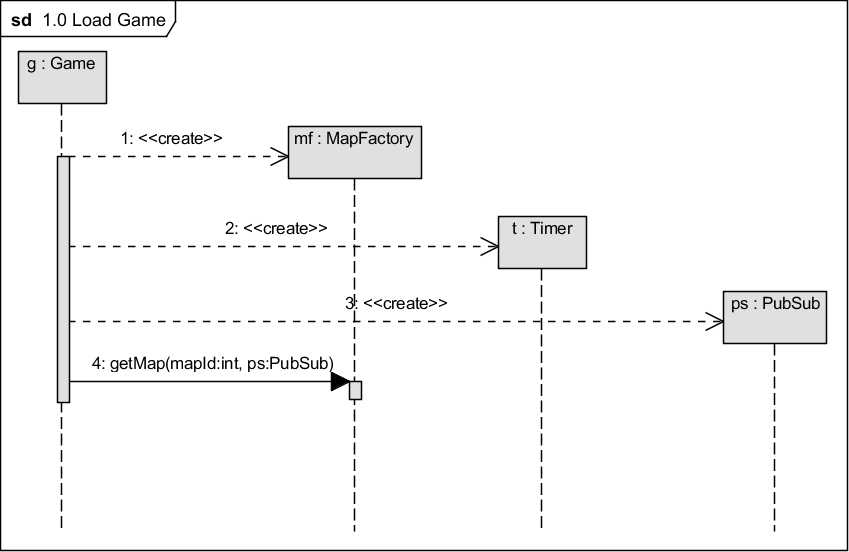
\includegraphics[scale=1]{resources/05/10LoadGame.png}\end{center}
		\begin{center}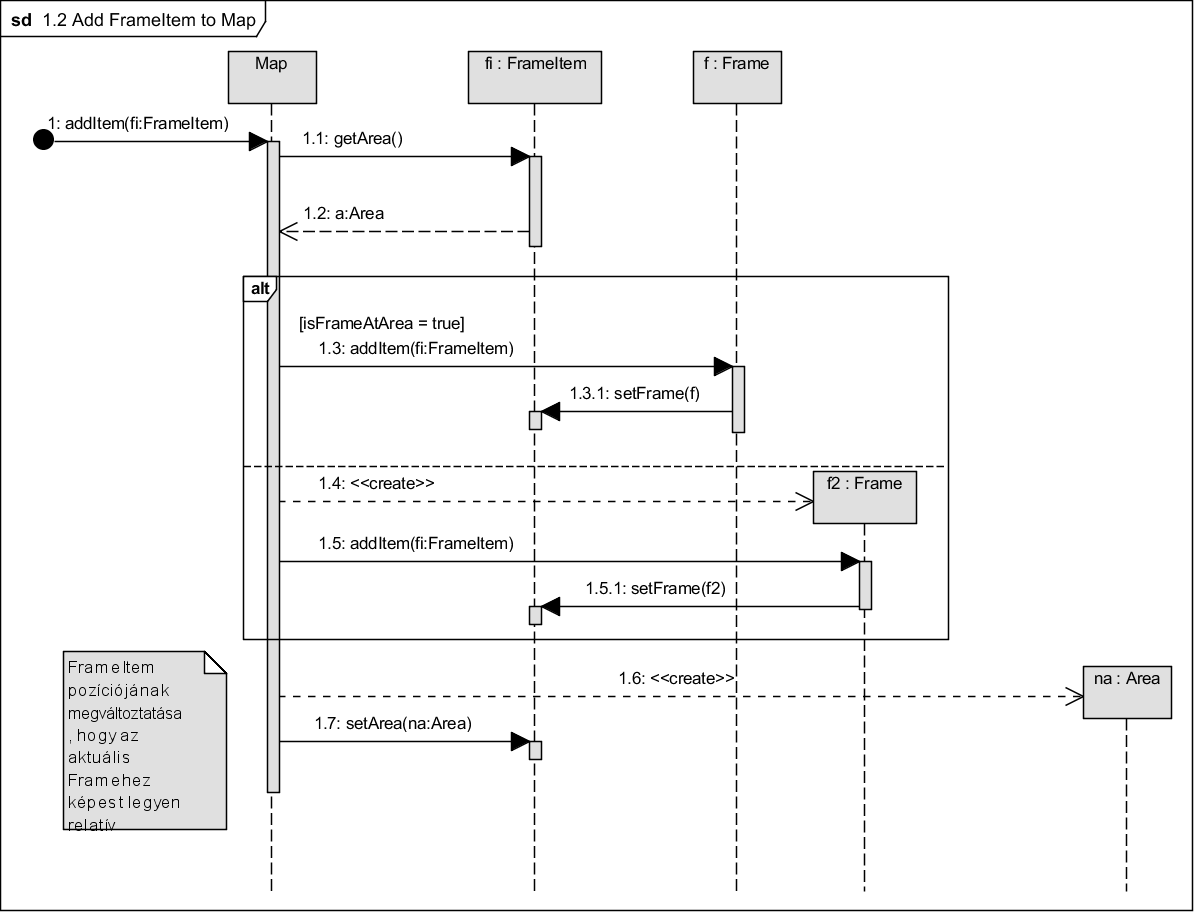
\includegraphics[scale=0.75]{resources/05/12AddFrameItemtoMap.png}\end{center}
		\begin{center}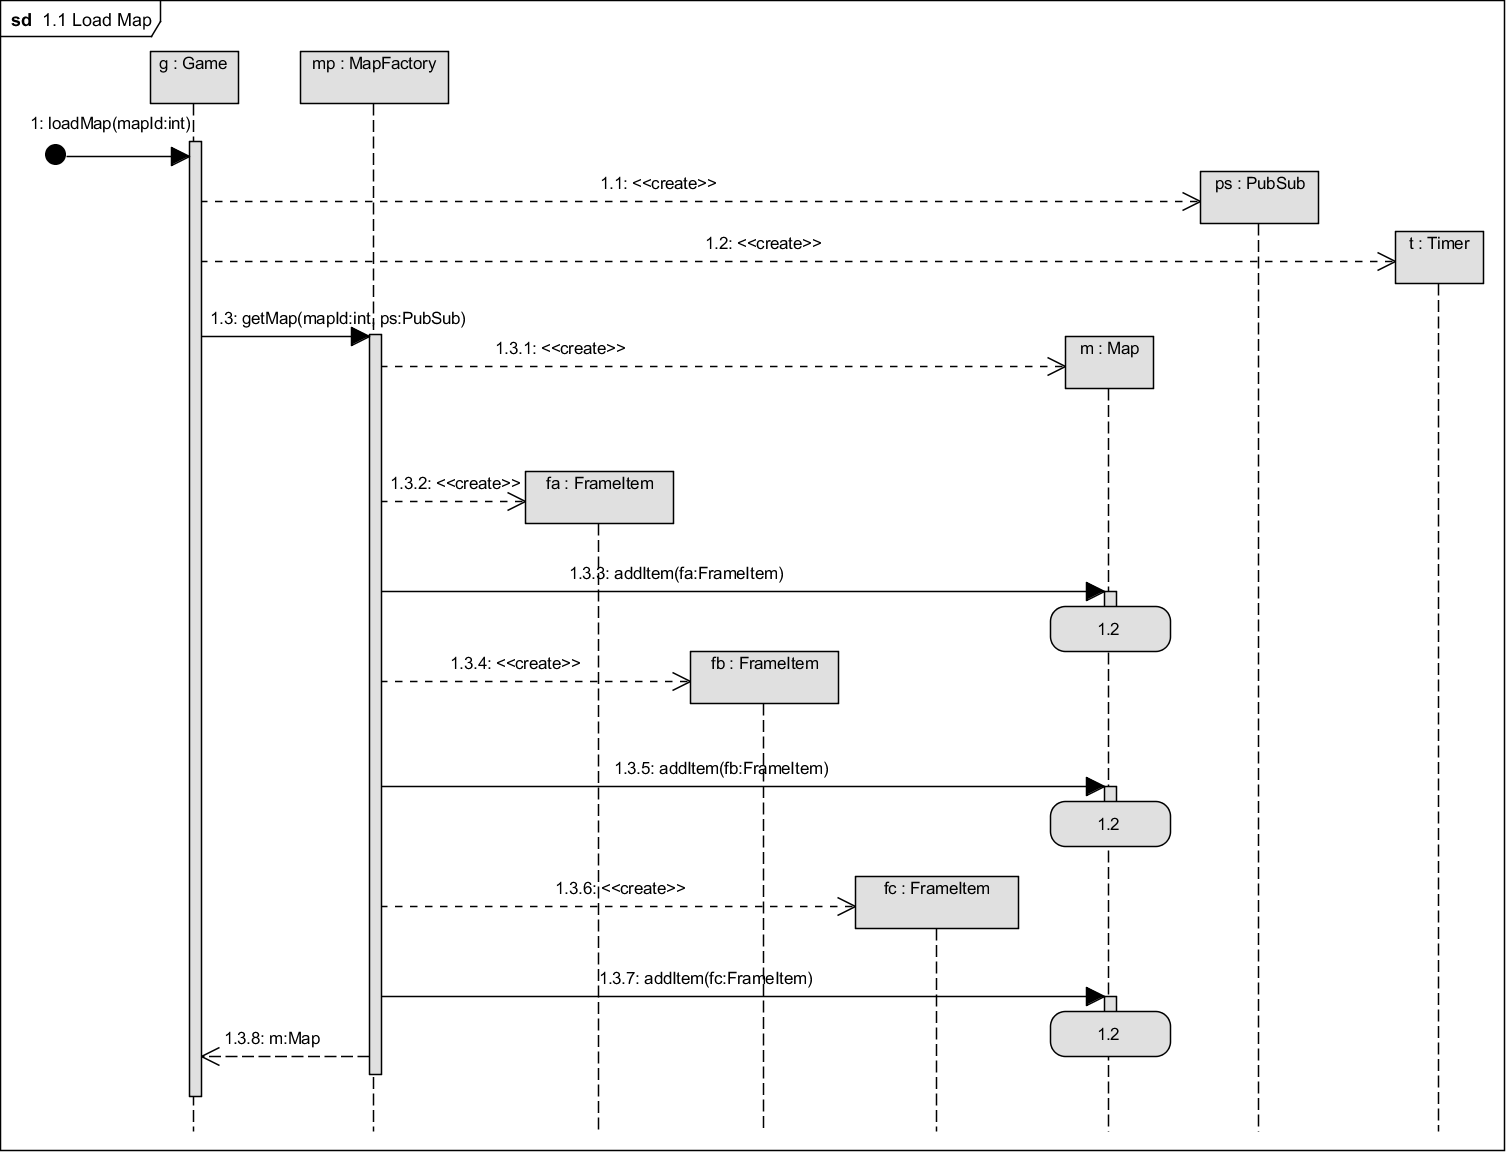
\includegraphics[scale=0.8, angle=-90]{resources/05/11LoadMap.png}\end{center}
		\begin{center}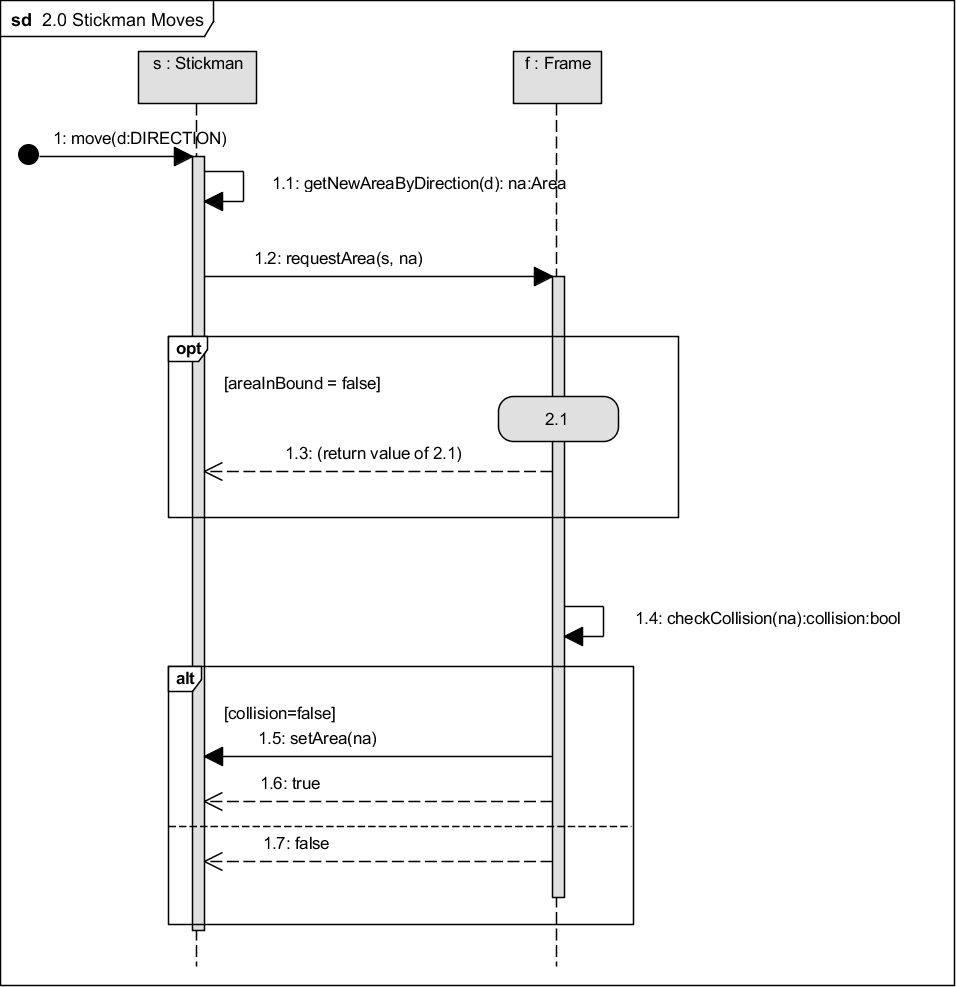
\includegraphics[scale=0.95]{resources/05/20StickmanMoves.png}\end{center}
		\begin{center}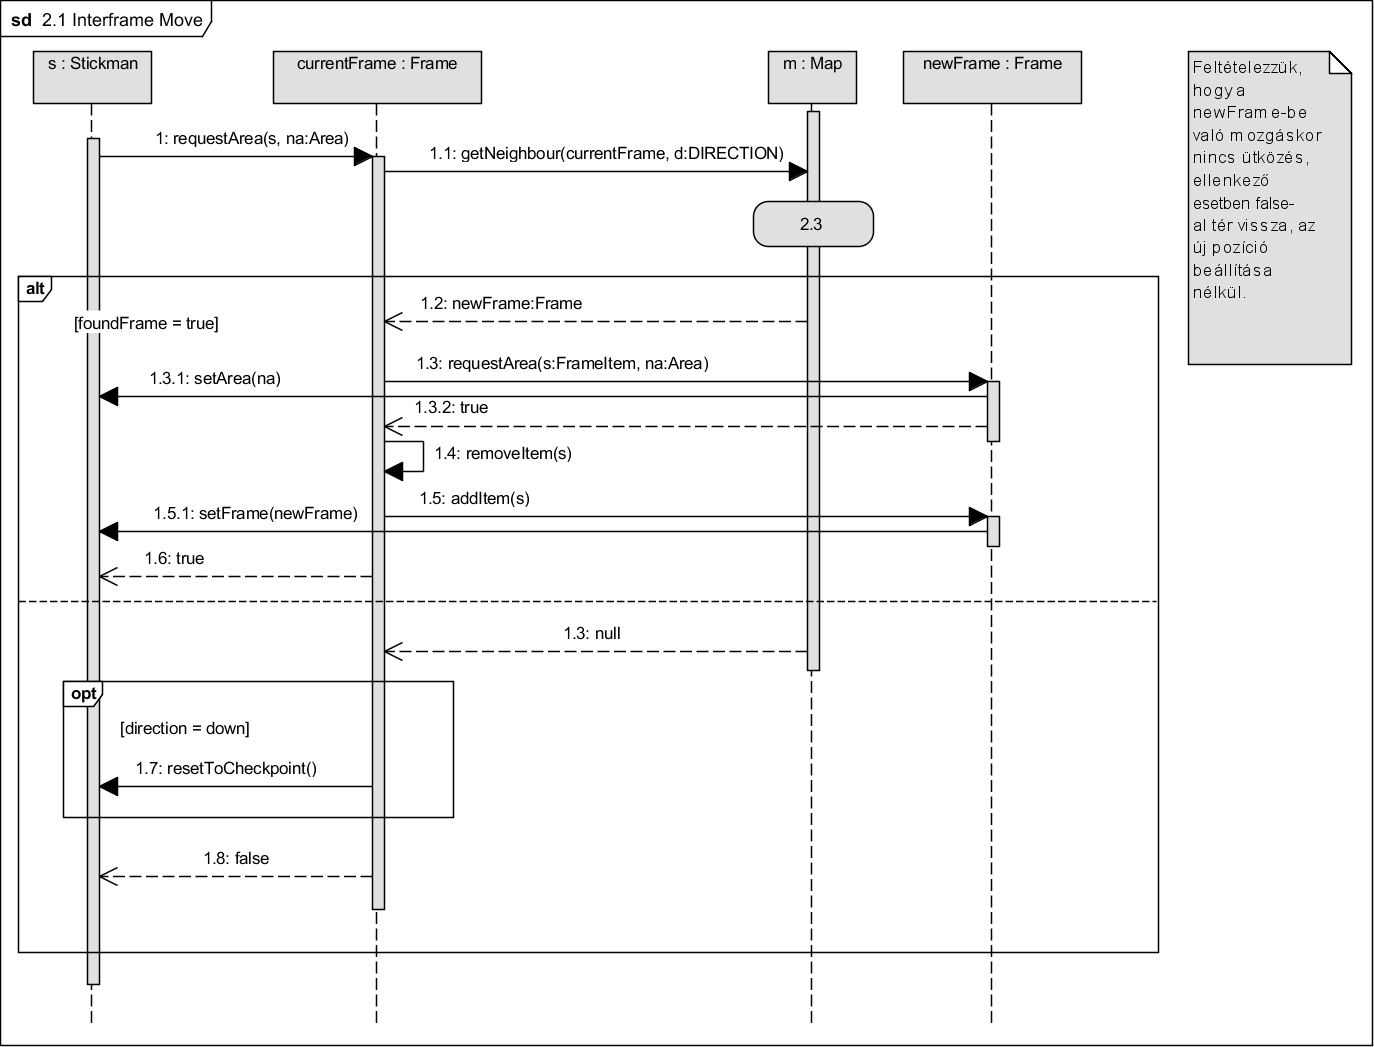
\includegraphics[scale=0.8, angle=-90]{resources/05/21InterframeMove.png}\end{center}
		\begin{center}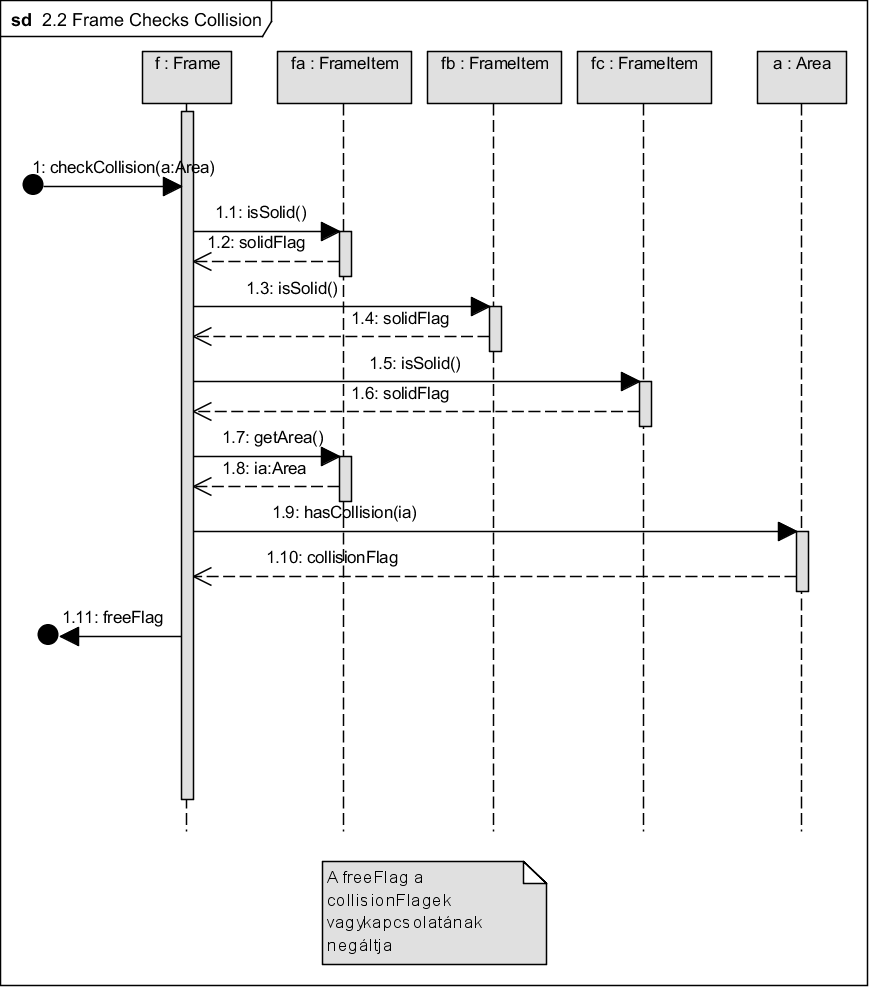
\includegraphics[scale=1]{resources/05/22FrameChecksCollision.png}\end{center}
		\begin{center}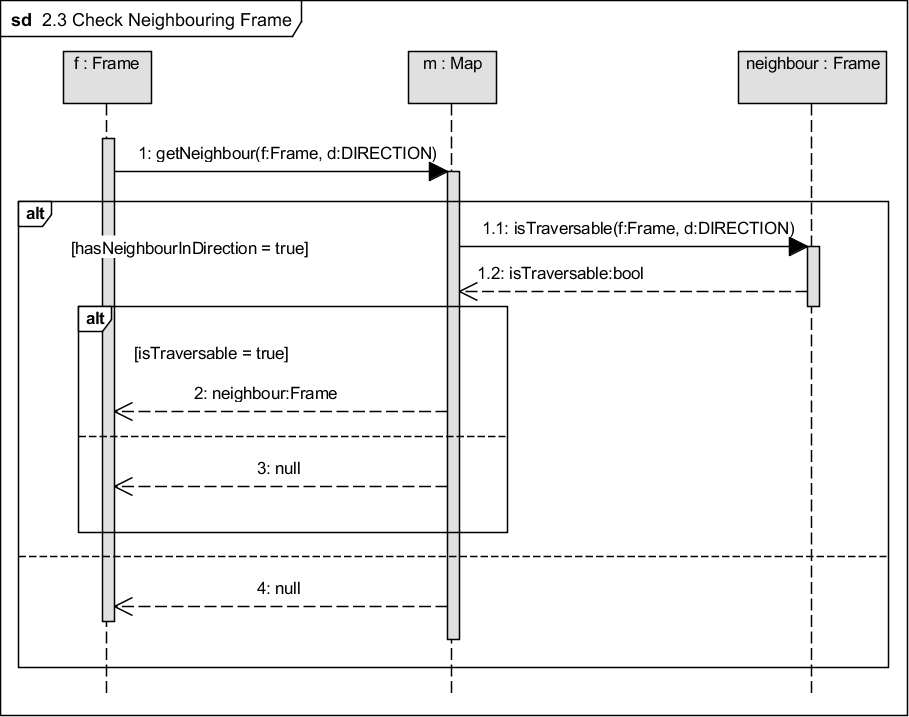
\includegraphics[scale=1]{resources/05/23CheckNeighbouringFrame.png}\end{center}
		\begin{center}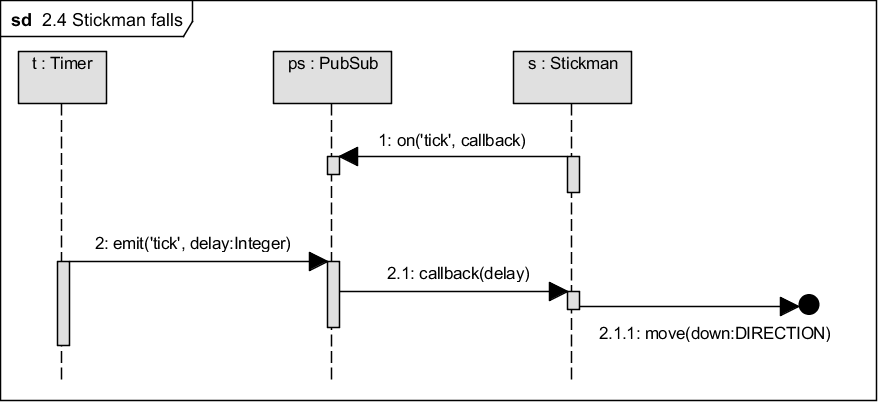
\includegraphics[scale=1]{resources/05/24Stickmanfalls.png}\end{center}
		\begin{center}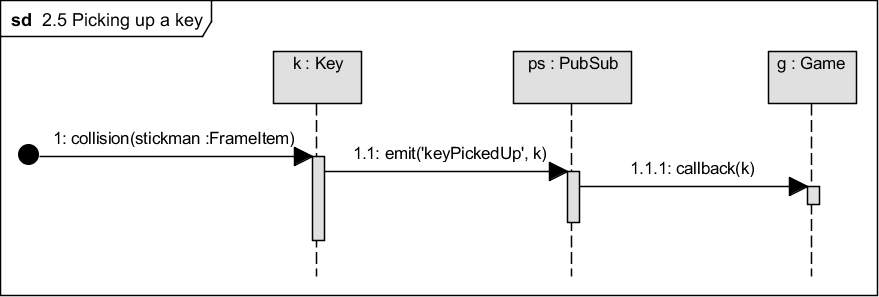
\includegraphics[scale=1]{resources/05/25Pickingupakey.png}\end{center}
		\begin{center}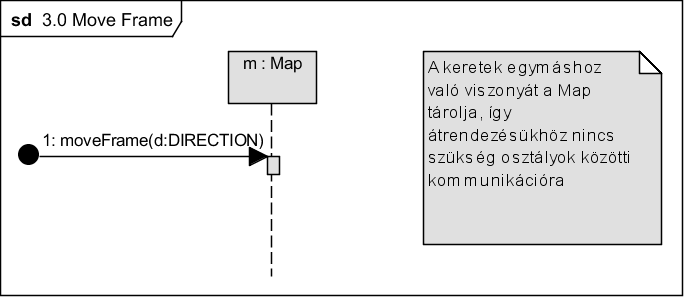
\includegraphics[scale=1]{resources/05/30MoveFrame.png}\end{center}
		\begin{center}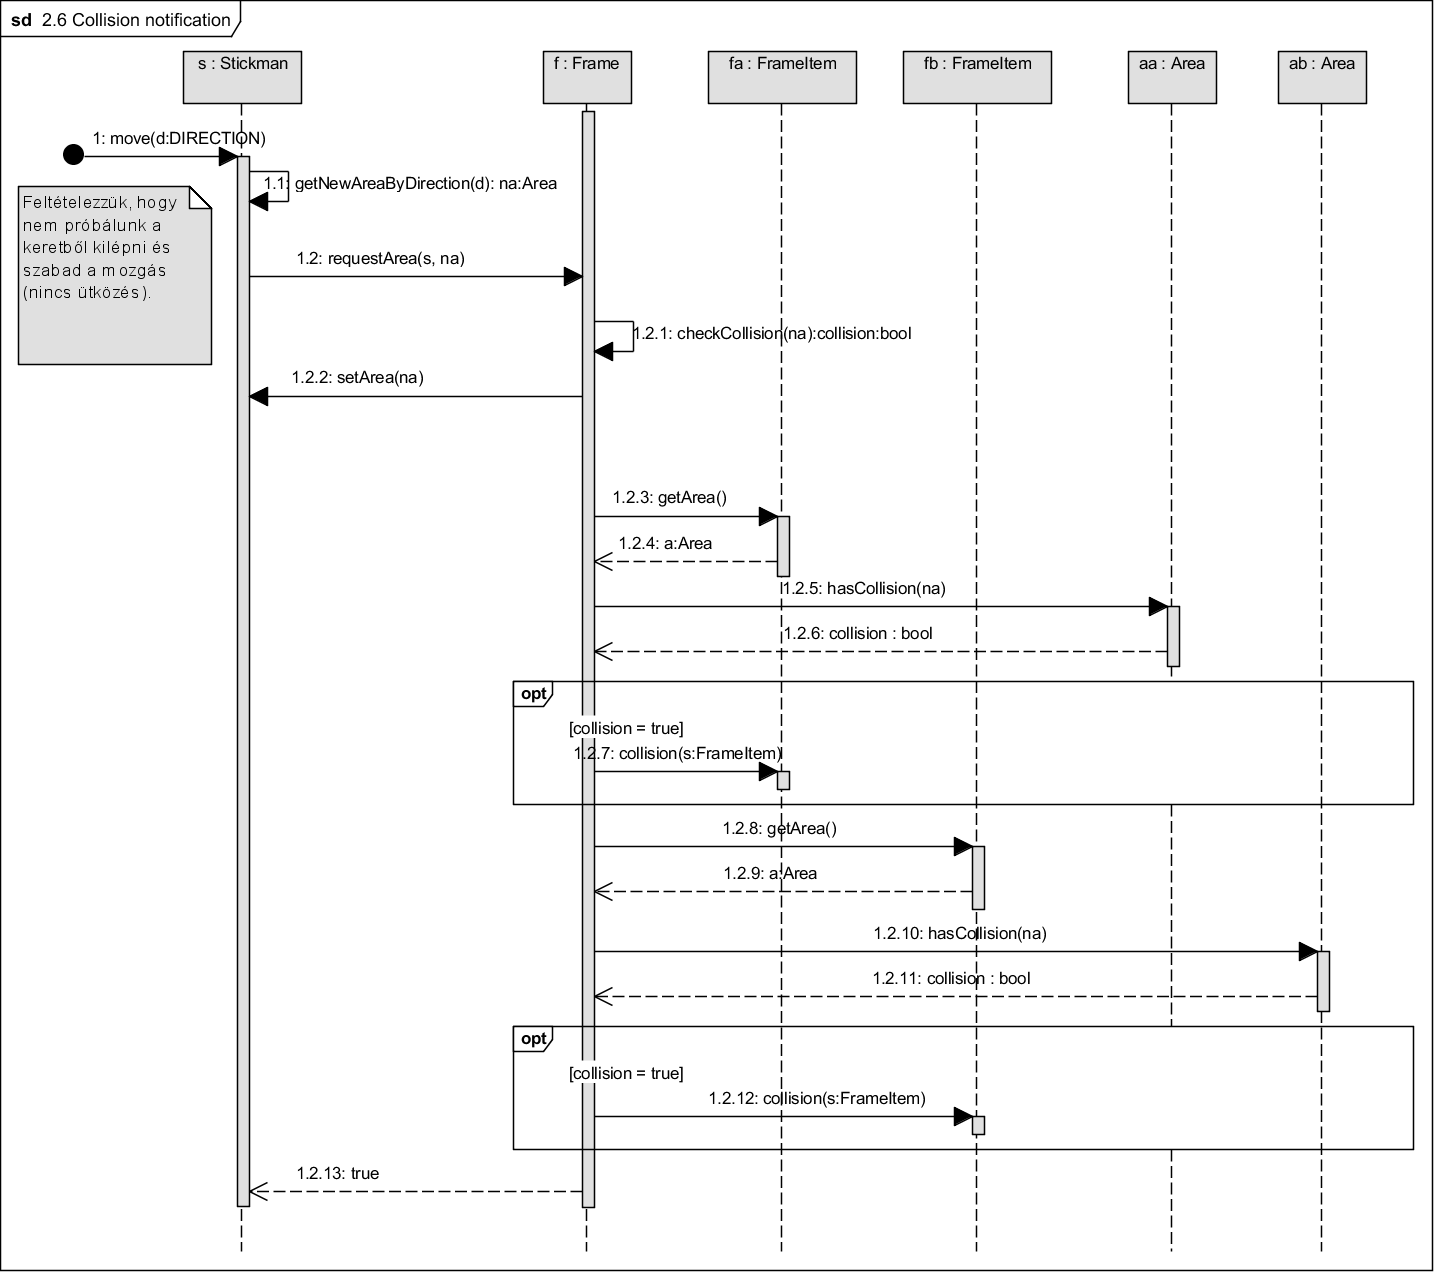
\includegraphics[scale=0.7, angle=-90]{resources/05/26Collisionnotification.png}\end{center}
	
	\subsection{Napló}
	% The diary generator uses the following comments to identify the beginning and the ending of the generated diary
	% The following content is auto generated, please do NOT modify, edit the related shared document instead.
	%GENERATOR:DIARY
    \begin{center} 
        \begin{tabular}{| l | p{1.9cm} | p{2.6cm} | p{6.1cm} |}
            \hline
                Kezdet & Időtartam & Résztvevők & Leírás \\
            \hline \hline 
2012. 03. 09. 17:00 & 3 óra & Berki & Szekvencia diagramok\\ \hline
2012. 03. 10. 18:00 & 2 óra & Fodor & A szkeleton kezelői felület tervének kidolgozása\\ \hline
2012. 03. 10. 21:20 & 2 óra & Kádár & Architektúra\\ \hline
2012. 03. 11. 11:30 & 2 óra & Thaler & Use case diagram\\ \hline
2012. 03. 11. 14:30 & 1 óra & Thaler & Use case diagram\\ \hline
2012. 03. 11. 15:30 & 1.5 óra & Kádár & Architektúra\\ \hline
2012. 03. 11. 22:00 & 1.5 óra & Thaler & Javítások, Napló, zárás\\ \hline
2012. 03. 11. 22:00 & 1.5 óra & Fodor & Javítások\\ \hline
2012. 03. 12. 08:30 & 0.5 óra & Kádár & Nyomtatás, átnézés\\ \hline

            \hline
        \end{tabular}
    \end{center}
	%GENERATOR:DIARY
\newpage
\section{Szkeleton tervezése}

	\subsection{Fordítási és futtatási útmutató}

		\subsubsection{Fájllista}
			\begin{center}
			    \begin{tabular}{ | l | l | l | p{5cm} |}
				    \hline
				    \textbf{Fájl neve}	& \textbf{Méret}	& \textbf{Keltezés ideje}	& \textbf{Tartalom} \\ \hline
				    %Autogenerated content, do not modify
                    %GENERATOR:FILE_LIST
					AbstractFrameItem.java	& 788 byte	& 2012. 03. 18. 18:33:55	& AbstractFrameItem osztály	\\ \hline
					AbstractTest.java	& 1158 byte	& 2012. 03. 17. 09:11:03	& Szkeleton tesztek ősosztálya	\\ \hline
					AddFrameItem    & 1580 byte	& 2012. 03. 18. 18:14:02	& 1.2 Add FrameItem to Map	\\ %\hline
					ToMapTest.java  &           &                           &                   \\ \hline
					Area.java	& 1832 byte	& 2012. 03. 18. 18:14:02	& Area osztály	\\ \hline
					DIRECTION.java	& 364 byte	& 2012. 03. 17. 08:53:43	& DIRECTION enumeráció	\\ \hline
					Door.java	& 1224 byte	& 2012. 03. 18. 18:14:02	& Door osztály	\\ \hline
					Frame.java	& 6348 byte	& 2012. 03. 18. 18:14:02	& Frame osztály	\\ \hline
					FrameItem.java	& 1229 byte	& 2012. 03. 17. 08:54:13	& FrameItem osztály	\\ \hline
					Game.java	& 1440 byte	& 2012. 03. 18. 18:45:31	& Game osztály	\\ \hline
					Key.java	& 2023 byte	& 2012. 03. 18. 18:33:33	& Key osztály	\\ \hline
					LoadGameTest.java	& 329 byte	& 2012. 03. 18. 18:14:02	& 1.0 Load Game teszt	\\ \hline
					LoadMapTest.java	& 509 byte	& 2012. 03. 18. 18:14:02	& 1.1 Load Map	\\ \hline
					Map.java	& 3180 byte	& 2012. 03. 18. 18:14:02	& Map osztály	\\ \hline
					MapFactory.java	& 1434 byte	& 2012. 03. 18. 18:14:02	& MapFactory osztály	\\ \hline
					PickupKeyTest.java	& 934 byte	& 2012. 03. 18. 18:31:23	& 2.5 Pick up a key	\\ \hline
					Platform.java	& 827 byte	& 2012. 03. 17. 08:55:00	& Platform osztály	\\ \hline
					PubSub.java	& 1762 byte	& 2012. 03. 18. 18:43:20	& PubSub osztály	\\ \hline
					SkeletonLogger.java	& 7961 byte	& 2012. 03. 18. 18:14:02	& Szkeleton kommunikáció követése	\\ \hline
					SkeletonRunner.java	& 4576 byte	& 2012. 03. 18. 18:14:02	& Szkeleton tesztek futtatókörnyezete	\\ \hline
					Stickman.java	& 2690 byte	& 2012. 03. 18. 18:14:02	& Stickman osztály	\\ \hline
					StickmanFalls.java	& 822 byte	& 2012. 03. 18. 18:51:52	& 2.4 Stickman Falls	\\ \hline
					StickmanMovesTest.java	& 618 byte	& 2012. 03. 18. 18:14:02	& 2.0 Stickman Moves	\\ \hline
					Subscriber.java	& 507 byte	& 2012. 03. 17. 08:55:28	& Subscriber interface	\\ \hline
					Test.java	& 241 byte	& 2012. 03. 17. 09:11:47	& Szkeleton tesztek interface	\\ \hline
					Timer.java	& 638 byte	& 2012. 03. 18. 18:14:02	& Timer osztály	\\ \hline

					%GENERATOR:FILE_LIST
			    \end{tabular}
			\end{center}

		\subsubsection{Fordítás}
		 A Szkeleton fordításának menete: a könyvtárszerkezet /skeleton mappájában állva a \\ \texttt{javac utils/*.java} \\ paranccsal lefordul a SkeletonLogger, majd \\ \texttt{javac model/*.java} \\
paranccsal lefordíthatóak a szükséges modellelemek, végül \\ \texttt{javac model/test/*.java} \\utasítással megtörténik a tesztek lefordítása. Ezzel a futtatható fájlok elkészítése megtörtént.

		\subsubsection{Futtatás}
		 A futtatható fájlok elkészítése után \\ \texttt{java model/SkeletonRunner} \\ paranccsal elindítható a teszteket összefogó program, mely a console-on keresztül valósítja meg a felhasználóval történő kommunikációt. \\
 	 A kipróbálható teszteseteket a program kilistázza, mindegyikhez egy számot rendelve, a felhasználó a billentyűzet segítségével adhatja meg a választott tesztesetet. Bizonyos tesztek működése során további interakció szükséges, ilyenkor a program ismét a felhasználó beavatkozására vár. A teszt lefolyásáról a console-on keresztül a felhasználó minden esetben részletes tájékoztatást kap. Egy teszt végrehajtása után a felhasználónak további tesztesetek kipróbálására van lehetősége, a programból való kilépés a '0' bemenenettel hajtható végre.

	\subsection{Értékelés}
		\begin{center}
		    \begin{tabular}{ | l | c |}
			    \hline
			    \textbf{Tag neve}	& \textbf{Munka százalékban} 	\\ \hline
				Berki Endre			& 20.26\%							\\ \hline			    
			    Fodor Bertalan		& 25.72\%							\\ \hline
			    Kádár András		& 22.51\%							\\ \hline
			    Thaler Benedek		& 31.51\%							\\ \hline
		    \end{tabular}
		\end{center}
	\subsection{Napló}
	% The diary generator uses the following comments to identify the beginning and the ending of the generated diary
	% The following content is auto generated, please do NOT modify, edit the related shared document instead.
	%GENERATOR:DIARY
    \begin{center} 
        \begin{tabular}{| l | p{1.9cm} | p{2.6cm} | p{6.1cm} |}
            \hline
                Kezdet & Időtartam & Résztvevők & Leírás \\
            \hline \hline 
2012. 03. 14. 08:00 & 1.5 óra & Fodor, Kádár, Thaler & Konzultáció\\ \hline
2012. 03. 14. 13:30 & 0.5 óra & Kádár & Előkészítés\\ \hline
2012. 03. 14. 15:00 & 0.5 óra & Thaler & Feladatkiosztás\\ \hline
2012. 03. 14. 15:30 & 1 óra & Thaler & Futtatókörnyezet\\ \hline
2012. 03. 14. 18:00 & 1.5 óra & Thaler & Futtatókörnyezet\\ \hline
2012. 03. 14. 20:00 & 0.5 óra & Thaler & Futtatókörnyezet\\ \hline
2012. 03. 16. 15:15 & 1 óra & Thaler & Build környezet\\ \hline
2012. 03. 17. 08:00 & 1.5 óra & Thaler & Teszt demo, dokumentáció\\ \hline
2012. 03. 17. 08:00 & 3 óra & Fodor & SkeletonLogger\\ \hline
2012. 03. 18. 11:00 & 3.5 óra & Kádár & Tesztesetek kódolása\\ \hline
2012. 03. 18. 15:10 & 0.5 óra & Kádár & Tesztesetek kódolása\\ \hline
2012. 03. 18. 16:10 & 1.5 óra & Kádár & Tesztesetek kódolása\\ \hline
2012. 03. 18. 18:00 & 1.5 óra & Thaler & Tesztesetek\\ \hline
2012. 03. 18. 18:00 & 4 óra & Berki & Dokumentáció, futtatókörnyezet\\ \hline
2012. 03. 18. 22:00 & 1 óra & Thaler & Csomagolás\\ \hline
2012. 03. 18. 22:15 & 1 óra & Berki & Átnézés, nyomtatás\\ \hline

            \hline
        \end{tabular}
    \end{center}
%GENERATOR:DIARY	
\newpage
\section{Prototípus koncepciója}

	\subsection{Prototípus interface-definíciója}
	%Definiálni kell a teszteket leíró nyelvet. Külön figyelmet kell fordítani arra, hogy ha a rendszer véletlen elemeket is tartalmaz, akkor a véletlenszerűség ki-bekapcsolható legyen, és a program determinisztikusan is tesztelhető legyen.
	    \subsubsection{Az interfész általános leírása}
	    %A protó (karakteres) input és output felületeit úgy kell kialakítani, hogy az input fájlból is vehető legyen illetőleg az output fájlba menthető legyen, vagyis kommunikációra csak a szabványos be- és kimenet használható.
	    A prototípus célja, hogy képet kapjunk a szkeletonban külön-külön tesztelt kommunikációs egységek integrálás utáni helyes működéséről. A prototípus egyrészről tehát egy integrációs teszt, másrészről viszont egyszerre egy működőképes program is, mely az egyszerűség érdekében nélkülözi a grafikus felületet, parancssoros kommunikációt használ. A felhasználó a tesztelés során a prototípussal parancsok útján léphet interakcióba, így befolyásolva annak futását. A parancsok futtatása után a kimenet összevethető a specifikációval.
	    
	    \subsubsection{Bemeneti nyelv}
	    %Definiálni kell a teszteket leíró nyelvet. Külön figyelmet kell fordítani arra, hogy ha a rendszer véletlen elemeket is tartalmaz, akkor a véletlenszerűség ki-bekapcsolható legyen, és a program determinisztikusan is futtatható legyen. A szálkezelést is tesztelhető, irányítható módon kell megoldani.
	    %Parancs1 \ Leírás: \ Opciók:
	    
	    A felhasználó a következő parancsok állnak rendelkezésére a tesztelés során:
	    
	    \newcommand{\cmd}[1]{\item{\texttt{#1}} }
	    \begin{description}
	        \cmd{timerStart}: Óraütések automatikus kiadásának bekapcsolása.
	        \cmd{timerStop}: Óraütések automatikus kiadásának kikapcsolása.
	        \cmd{tick} \emph{count}: Megadott számú öraütést szimulál.
	        \cmd{loadMap} \emph{mapId}: Megadott pálya betöltése.
	        \cmd{move} \emph{stickmanId} \emph{direction}: A megadott azonosítójú stickman megfelelő irányba mozgatása (up, right, down, left).
	        \cmd{viewportSwitch}: Pálya és közeli nézet közötti váltás.
	        \cmd{moveFrame} \emph{direction}: Keret mozgatása pályanézetben a megadott irányba (up, right, down, left).
	        \cmd{echoCommands} \emph{status}: Bemeneti parancsok kiírása a kimenetre a könnyebb debuggolás kedvéért. (status: true vagy false)
        \end{description}
        
        A parancsokat a program a szabványos bemenetről olvassa be, így tetszőleges fájl beállítható a parancsok forrásának, ha a megfelelő fájlt a bemenetre irányítjuk.
        
        \subsubsection{Pálya fájlreprezentációja}
        %Ha szükséges, meg kell adni a konfigurációs (pl. pályaképet megadó) fájlok nyelvtanát is.
        A felhasznált pályákat a program fájlokból olvassa be, melyek felépítése a következő: A fájlok soralapúak, minden sor egy objektumot kódol a pályán. A sor elején a konkért objektumot azonosító név áll, majd egy tabulátorral elválasztva következnek a paraméterei. A különböző objektumok tetszőleges számú paramétert vehetnek át, mely paramétereket tabulátorral elválasztva kell az objektum neve után felsorolni. Minden, a pályán szereplő objektum első 4 paramétere (ha specifikált), rendre a következő attribútumokat kódolja: Pálya bal felső sarkától számított (abszolút) x irányú eltolás, y irányú eltolás, objektum szélessége, objektum magassága. A pálya fájlban a következő objektumnevek szerepelhetnek: \texttt{Door, Key, Platform, Stickman}. A pályán található keretek számának és elhelyezkedésének megadására nincs szükség, azt a program az elhelyezett elemek pozíciója alapján dinamikusan építi fel.
        
	    \subsubsection{Kimeneti nyelv}	
	    %Egyértelműen definiálni kell, hogy az egyes bemeneti parancsok végrehajtása után előálló állapot milyen formában jelenik meg a szabványos kimeneten.	
	    A karakteres kimeneten minden -- a modell állapotának változását okozó -- esemény, valamint bármely parancs után megjelenik a modell aktuális állapotát reprezentáló szöveges ábra. Alapértelmezetten nem, de az \texttt{echoCommands} parancs használatával a megadott parancs is kiírásra kerül pályarajz után, így segítve a kimenet követését, ha azt fájlba írtuk. A pálya szöveges reprezentációját képező ábrán a következő szimbólumok fordulhatnak elő:
	    
	    \begin{description}
	        \newcommand{\frameitem}[1]{\item{\textbf{#1}} }
	        % pdflatex doesn't accept the following symbols, use simpler ones
	        % ☺, ☻, █, ⚷, ☐
	        \frameitem{X, Y}: A stickmanek
	        \frameitem{|, --, +}: Keret függőleges széle, keret vízszintes széle, keret sarka
	        \frameitem{\#}: Platform
	        \frameitem{K}: Kulcs
	        \frameitem{A}: Ajtó
        \end{description}

        A pálya szöveges reprezentációja például az alábbi formát öltheti:
        
		\begin{figure}[hb]
		  \begin{center}
		  % let me introduce the centering of dummy people
		\begin{verbatim}
                +----------+ +----------+ +----------+
                |          | |        ##| |#        #|
                |  X##   ##| |##        | |#   K     |
                |##########| |##########| |##########|
                +----------+ +----------+ +----------+
                +----------+ +----------+
                |##   K    | |##     ###|
                |    ##    | |    Y   A |
                |##########| |##########|
                +----------+ +----------+
		\end{verbatim}
		  \caption{A pálya szöveges reprezentációja}
		  \end{center}
		\end{figure}        
        
        Mivel a program a kimenetét sztandard kimenetre írja ki, így az egyszerűen elemezhető a konzolon vagy írható fájlba. Amennyiben egy stickman megérint egy kulcsot, a kulcs eltűnik és a megszerzője tulajdonába kerül.
	
	\subsection{Összes részletes use-case}
        %domain specific commands
        \renewcommand{\ucitem}[1]{\item \textbf{Név: #1}\\}
        \renewcommand{\ucdesc}[1]{\textbf{Rövid leírás: } #1\\}
        \newcommand{\ucact}[1]{\textbf{Actor: } #1\\}
        \renewcommand{\ucscenario}[1]{\textbf{Forgatókönyv: }#1\\}
        
		\begin{center}	
		    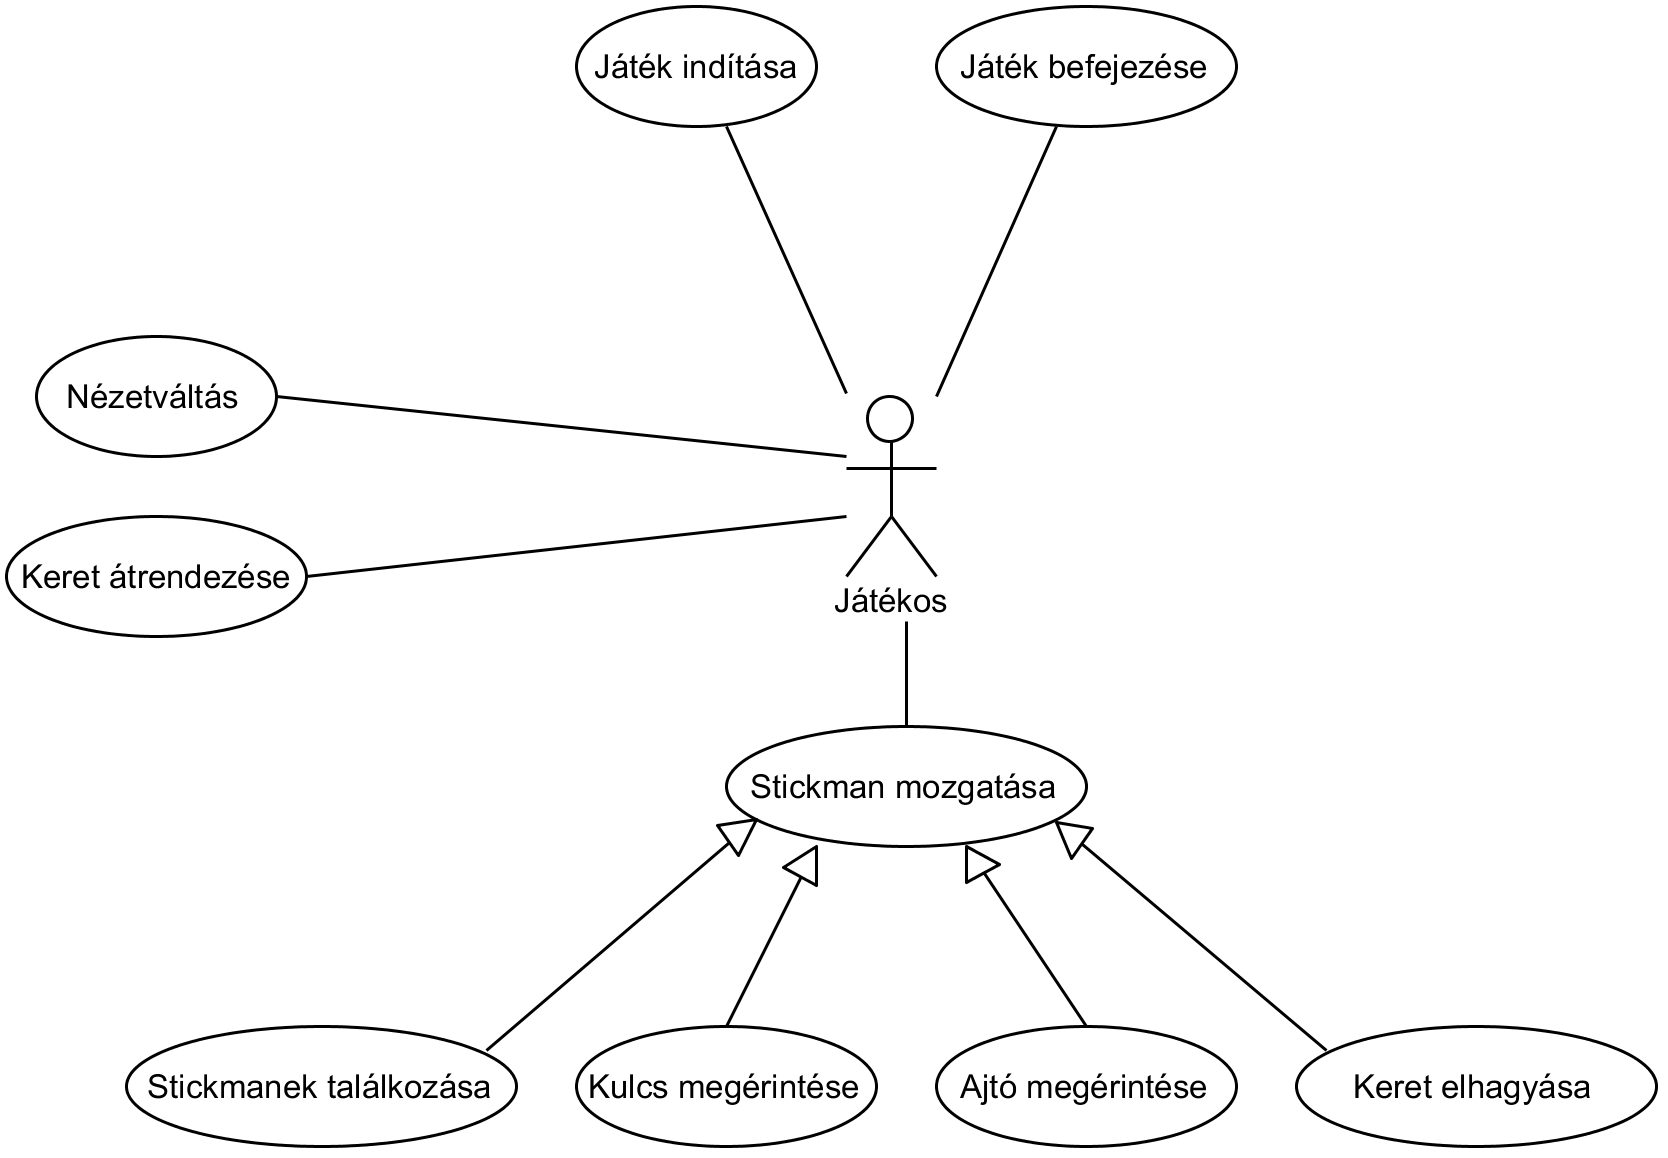
\includegraphics[scale=0.9]{resources/07/player.png}
		\end{center}        
        
        \subsubsection{Irányításhoz kapcsolódó use-case-ek} 
		
	    \begin{enumerate}[label=\textbf{\arabic*.}, start=1]
	        \ucitem{Játék indítása} 
	        \ucdesc{A felhasználó elindítja a játékot.} 
	        \ucact{Játékos}
	        \ucscenario{A pálya betöltődik, a stickmanek és a többi elem elhelyezésre kerül a pályán.} 

		
	        \ucitem{Játék befejezése} 
	        \ucdesc{Kilépés a játékból.} 
	        \ucact{Játékos}
	        \ucscenario{Az utolsó mentett pozíció alapján a játék mentése. Fájlok lezárása és kilépés a programból.} 
	        
	        \ucitem{Stickman mozgatása} 
	        \ucdesc{Játékos irányítja az egyik Stickmant.} 
	        \ucact{Játékos}
	        \ucscenario{A lehetséges irányok: jobbra, balra, fel(ugrás). Amennyiben a mozgás irányában van szabad terület, a pozíciója megváltozik, egyébként blokkolódik (helyben marad)}
		
	        \ucitem{Nézetváltás} 
	        \ucdesc{A játékos nézetet vált.} 
	        \ucact{Játékos}
	        \ucscenario{Ha közeli nézetben volt, akkor pálya nézetbe lép, ahol látja a kereteket. Ekkor a Stickman irányítása letiltódik és a keret átrendezés irányítása aktiválódik. Ha pálya nézetben volt, akkor fordítva.} 
	        
	        \ucitem{Keret átrendezése} 
	        \ucdesc{Pálya nézetben a keretek átrendezése.} 
	        \ucact{Játékos}
	        \ucscenario{A megadott irányok mentén a keretek átrendezhetőek, mindig az üres kerettel helyet cserélve} 
	    \end{enumerate}
	    
        \subsubsection{Időhöz kapcsolódó use-case-ek} 
		
	    \begin{enumerate}[label=\textbf{\arabic*.}, start=1]
	        \ucitem{Idő léptetése} 
	        \ucdesc{Jelzi az idő múlását.} 
	        \ucact{Óra}
	        \ucscenario{Számítógép által vezérelt idő léptetés, amely a Stickman vertikális pozícióját befolyásolja.} 
	    \end{enumerate}
	    
        \subsubsection{Stickman(ek)hez kapcsolódó use-case-ek} 

	    \begin{enumerate}[label=\textbf{\arabic*.}, start=1]
	    
	        \ucitem{Stickmanek találkozása} 
	        \ucdesc{Két Stickman mozgásuk során találkozik.} 
	        \ucact{Játékos}
	        \ucscenario{A két Stickman ütközik egymással, mint két szilárd objektum, de további interakció nem történik} 
		
	        \ucitem{Kulcs megérintése} 
	        \ucdesc{A Stickman mozgása során felvesz egy kulcsot.} 
	        \ucact{Játékos}
	        \ucscenario{A kulcs a stickmanhez kerül és eltűnik a pályáról}
		
	        \ucitem{Ajtó megérintése}
	        \ucdesc{A Stickman mozgása során egy ajtóhoz ér.}
	        \ucact{Játékos}
	        \ucscenario{Amennyiben minden kulcsot megszereztek, akkor vége a pályának, egyébként a Stickman elhalad az ajtó előtt.}

	        \ucitem{Keret elhagyása} 
	        \ucdesc{A Stickman valamely irányba elhagyja az aktuális keretet} 
	        \ucact{Játékos}
	        \ucscenario{Amennyiben van szomszédos keret és a két keret átjárható, a stickman belép az új keretbe. Amennyiben a szomszédos keret nem átjárható, akkor ha a célkeret alsószomszéd, a stickman kiesik, egyébként blokkolódik (helyben marad).}
	        
	    \end{enumerate}
	    
    	\subsection{Tesztelési terv}
			\newcommand{\testitem}[1]{\item \textbf{Név: #1}\\}
			\newcommand{\tdesc}[1]{\textbf{Leírás: } #1\\}
			\newcommand{\tcel}[1]{\textbf{Cél:} #1\\}
	
			\begin{enumerate}[label=\textbf{\arabic*.}, start=1]
%			    \testitem{}
%		        \tdesc{}
%		        \tcel{}
		        
		        \testitem{Pálya betöltése}
		        \tdesc{Betöltésre kerül egy objektumokkal feltöltött pálya, melyet a \texttt{MapFactory} készít el a pálya fájlreprezentációja alapján, és elhelyezi rajta a stickmaneket.}
		        \tcel{Ellenőrizni, hogy a pálya fájlreprezentációjából helyes pályakép generálódik a programban, minden objektum a helyén van-e. \texttt{MapFactory}-nak létre kell hoznia a megfelelő számú \texttt{Frame}-et és azokat helyesen elhelyezni, valamint létre kell hoznia a \texttt{FrameItem}eket.}
		        
		        \testitem{Stickman mozgatása kereten belül}
		        \tdesc{Az egyik stickmant megmozgatjuk kereten belül minden irányba: vízszintesen és horizontálisan (felfele), úgy hogy van tereptárgy a mozgás irányában, mely azt megakadályozza, és úgy is hogy nincs, illetve leugrunk vele egy magaslatról.}
		        \tcel{Ellenőrizni, hogy a kiadott mozgatási parancsok a várt helyre viszik-e a stickmant, a tereptárgyak megakadályozzák-e a mozgását, ill. hogy az ugrás helyesen működik-e (a parancs kiadása után az idő múlása során először fölfele mozog, majd megáll, lefele mozog, és talajt érve újra megáll). A teszt során a \texttt{Stickman} \texttt{area} attribútuma áll középpontban, illetve hogy a \texttt{PubSub}-ból jövő \texttt{tick} események hatására hogyan reagál.}
		        
		        \testitem{Stickman mozgatása keretek között}
		        \tdesc{A Stickmant először olyan keretek között mozgatjuk, melyek átjárhatóak, majd egy olyanba próbáljuk vezérelni, ahova nincs lehetősége átmenni.}
		        \tcel{Keretek közti átjárhatóság megállapítását végző algoritmus, ill. a \texttt{Stickman} egyik \texttt{Frame}-ből másikba való áthelyezésének ellenőrzése. \texttt{Frame} kérésére a \texttt{Map} visszaadja a szomszédos \texttt{Frame}-et, és az előbbi \texttt{Frame} átrakja oda a \texttt{Stickman}t.}
		        
		        \testitem{Stickman kiesése}
		        \tdesc{Stickmant úgy vezéreljük, hogy essen ki egy keret alján úgy, hogy arra nincs több keret, vagy afelé a keret nem átjárható.}
		        \tcel{Ellenőrizzük, hogy a {Stickman} kiesik-e, ha a játék szabályai szerint ki kell esnie, illetve megnézzük, hogy ilyenkor visszakerül-e az utolsó ellenőrzőponthoz. Az aktuális \texttt{Frame} elkéri a \texttt{Map}től a szomszédját, melyre az \texttt{null} értékkel válaszol, erről pedig értesíti a \texttt{Stickmant}.}
		        
		        \testitem{Kulcs felvétele, pálya teljesítése}
		        \tdesc{Stickmannel először megérintjük az ajtót, ezután felvesszük a kucsot, majd megint megérintjük az ajtót.}
		        \tcel{Ellenőrizzük, hogy az ajtó csak kulccsal nyitható-e, illetve hogy a kulcs felvétele megfelelően rögzítődik-e. A teszt középpontjában a \texttt{Frame} által megvalósított ütközésértesítés áll, illetve az állapotok rögzítése, mely a \texttt{PubSub}-on jövő értesítés után a \texttt{Game}-ben történik.}
		        
		        \testitem{Keret mozgatása}
		        \tdesc{Távoli nézetben keret mozgatása parancsot adunk ki.}
		        \tcel{Ellenőrizzük, hogy a keret mozgatása parancs hatására a \texttt{Map} a megfelelő \texttt{Frame}-et mozgatja és azt a megfelelő helyre viszi.}
		        
		        \testitem{Nézetek közötti váltás}
		        \tdesc{A pálya betöltése után a kezdeti távoli nézetből közelibe váltunk. Itt ugrunk egyet, majd megpróbáljuk a kereteket átrendezni, ami nem sikerül. Esünk egyet, mely közben távoli nézetbe váltunk. Ekkor megpróbáljuk vízszintesen mozgatni a stickmant, ami nem sikerül.}
		        \tcel{Ellenőrizzük, hogy a stickman mozgatása le van-e tiltva távoli nézetben, illetve a keretek mozgatása közeli nézetben. Megnézzük még, hogy az időzítés helyesen működik-e, a kiadott \texttt{tick} parancs ellenére sem esik tovább a \texttt{Stickman} távoli nézetben.}
			\end{enumerate}
	    	
	\subsection{Tesztelést támogató segéd- és fordítóprogramok specifikálása}		
A tesztelés során keletkező kimenetek összehasonlítása az előre definiált kimenetekkel nem kézi erővel történik, erre a unix(-like) rendszereken megtalálható \texttt{diff} -- vagy azzal azonos funkcionalitású, más platformon futó -- programot fogunk használni. Egy teszteset akkor tekinthető sikeresnek, ha a \texttt{diff} program nem jelez különbséget a kapott kimenet és az előre definiált kimenet között.

	\subsection{Napló}
	% The diary generator uses the following comments to identify the beginning and the ending of the generated diary
	% The following content is auto generated, please do NOT modify, edit the related shared document instead.
	%GENERATOR:DIARY
    \begin{center} 
        \begin{tabular}{| l | p{1.9cm} | p{2.6cm} | p{6.1cm} |}
            \hline
                Kezdet & Időtartam & Résztvevők & Leírás \\
            \hline \hline 
2012. 03. 20. 17:00 & 4 óra & Thaler & Prototípus tervezés\\ \hline
2012. 03. 21. 14:00 & 3 óra & Thaler & Prototípus kialakítás\\ \hline
2012. 03. 24. 08:00 & 0.5 óra & Thaler & Inicializálás\\ \hline
2012. 03. 24. 19:45 & 3 óra & Thaler & Interface def\\ \hline
2012. 03. 24. 22:00 & 1.5 óra & Fodor, Kádár, Thaler & Team meeting\\ \hline
2012. 03. 25. 11:00 & 0.5 óra & Fodor & Tesztelési terv\\ \hline
2012. 03. 25. 12:00 & 2 óra & Kádár & Use case-ek\\ \hline
2012. 03. 25. 14:00 & 4 óra & Thaler & Prototípus felület\\ \hline
2012. 03. 25. 15:00 & 3 óra & Fodor & Tesztelési terv\\ \hline
2012. 03. 25. 20:30 & 1 óra & Thaler & Takarítás, csomagolás\\ \hline
2012. 03. 25. 21:00 & 0.5 óra & Fodor & Dokumentum átnézése\\ \hline
2012. 03. 25. 21:30 & 0.5 óra & Kádár & Use case javítás\\ \hline
2012. 03. 26. 00:00 & 1 óra & Berki & Nyomtatás, minőségellenőrzés\\ \hline

            \hline
        \end{tabular}
    \end{center}
%GENERATOR:DIARY
\newpage
\section{Szkeleton tervezése}
	\subsection{Osztályok és metódusok tervei}
%GENERATOR:CLASS_DESCRIPTIONS
		\subsubsection{AbstractFrameItem} Absztrakt osztály.
			\begin{description}

				\item[Felelősség] Alapértelmezett megvalósítása egy keretben lévő objektumnak.

				\item[Ősosztályok] (nincs)
				\item[Interfészek] FrameItem.
				\item[Attribútumok]$\ $
					\begin{description}
						\item[\texttt{\#area : Area}]A tartalmazó kereten belül elfoglalt pozíció
						\item[\texttt{\#frame : Frame}]A tartalmazó keret
						\item[\texttt{\#pubSub : PubSub}]Publish Subscribe channel
					\end{description}
				\item[Metódusok]$\ $
					\begin{description}
						\item[\texttt{+collision(colliding : FrameItem)}] \hfill \\Nem csinál semmit ütközés esetén    Alapértelmezetten az elemek nem reagálnak az ütközésre.  E metódus felüldefiniálásával ez a viselkedés megváltoztatható. 
						\item[\texttt{+doesAffectTraversability() : boolean}] \hfill \\Megadja, hogy számba kell-e venni az elemet,  ha a keretek közötti átjárást vizsgáljuk. 
						\item[\texttt{+getArea() : Area}] \hfill \\Visszaadja az elem pozícióját a kereten belül. 
						\item[\texttt{\#invalidate()}] \hfill \\Jelzés kibocsájtása az elem állapotának megváltozásáról 
						\item[\texttt{+setArea(area : Area)}] \hfill \\Beállítja az elem pozícióját a kereten belül. 
						\item[\texttt{+setFrame(frame : Frame)}] \hfill \\Beállítja az elemet tartalmazó keretet. 
						\item[\texttt{+setPubSub(pubSub : PubSub)}] \hfill \\Kommunikációs csatorna beállítása 
					\end{description}
			\end{description}

		\subsubsection{Area}
			\begin{description}

				\item[Felelősség] Területrészt leíró osztály. Összehasonlítható egy másik osztállyal, hogy fedik-e egymást.

				\item[Ősosztályok] (nincs)
				\item[Interfészek] (nincs)
				\item[Attribútumok] (nincs)
				\item[Metódusok]$\ $
					\begin{description}
						\item[\texttt{+clone() : Area}] \hfill \\Létrehoz egy új területet, magával megegyező paraméterekkel    A másolt paraméterek: x, y, height, width. 
						\item[\texttt{+getHeight() : int}] \hfill \\Megadja a terület magasságát 
						\item[\texttt{+getRelativeDirection(area : Area) : DIRECTION}] \hfill \\ Kiszámolja az adott terület relatív irányát. Egyszerre csak egy dimenziót vesz figyelembe. Ha a területek átlósan vannak elhelyezve, a vízszintes iránnyal tér vissza.
						\item[\texttt{+getWidth() : int}] \hfill \\Megadja a terület szélességét 
						\item[\texttt{+getX() : int}] \hfill \\Megadja a terület bal felső sarkának x eltolását 
						\item[\texttt{+getY() : int}] \hfill \\Megadja a terület bal felső sarkának y eltolását    Az eltolás felülről lefelé nő 
						\item[\texttt{+hasCollision(other : Area) : boolean}] \hfill \\Ellenőrzi, hogy a kapott Area objektummal van-e közös pontja.  A metódus feltételezi, hogy a két terület azonos keretben található. 
						\item[\texttt{+setHeight(height : int)}] \hfill \\Beállítja a terület magasságát 
						\item[\texttt{+setWidth(width : int)}] \hfill \\Beállítja a terület szélességét 
						\item[\texttt{+setX(x : int)}] \hfill \\Beállítja a terület bal felső sarkának x eltolását 
						\item[\texttt{+setY(y : int)}] \hfill \\Beállítja a terület bal felső sarkának y eltolását    Az eltolás felülről lefelé nő 
					\end{description}
			\end{description}

		\subsubsection{DIRECTION}
			\begin{description}

				\item[Felelősség] Irányokat jelöl a két dimenziós térben.

				\item[Ősosztályok] Enum $\rightarrow{}$ DIRECTION
				\item[Interfészek] (nincs)
				\item[Attribútumok]$\ $
					\begin{description}
						\item[\texttt{+\underline{DOWN : DIRECTION}}]% TODO
						\item[\texttt{+\underline{LEFT : DIRECTION}}]% TODO
						\item[\texttt{+\underline{RIGHT : DIRECTION}}]% TODO
						\item[\texttt{+\underline{UP : DIRECTION}}]% TODO
					\end{description}
				\item[Metódusok] (nincs)
			\end{description}

		\subsubsection{Door}
			\begin{description}

				\item[Felelősség] Ajtó objektum, melyet ha megérint a Stickman arról esemény bocsát ki.

				\item[Ősosztályok] AbstractFrameItem $\rightarrow{}$ Door
				\item[Interfészek] (nincs)
				\item[Attribútumok] (nincs)
				\item[Metódusok]$\ $
					\begin{description}
						\item[\texttt{+collision(colliding : FrameItem)}] \hfill \\A tartalmazó keret jelezheti ezen a metóduson keresztül,  hogy egy másik elem, melyet paraméterül ad,  hozzáért (collision) ehhez az elemhez.    A megérintésének tényét jelzi a kommunikációs csatornán,  hogy -- amennyiben minden kulcs össze van gyűjtve --  lehetővé váljon a pálya teljesítése. 
						\item[\texttt{+isSolid() : boolean}] \hfill \\Megadja, hogy az elem szilárd-e vagy sem.  Ez a kereten belüli mozgások esetén az  ütközések ellenőrzésekor használatos. 
					\end{description}
			\end{description}

		\subsubsection{Frame}
			\begin{description}

				\item[Felelősség] A pálya által alkotott táblázat egy cellája, amely elemeket tartalmaz. Ez felelős az elemek (Stickman) mozgatásáért kereten belül és között egyaránt. Két elem egy helyen való tartózkodásáról értesíti az elemeket (collision notify).

				\item[Ősosztályok] (nincs)
				\item[Interfészek] (nincs)
				\item[Attribútumok]$\ $
					\begin{description}
						\item[\texttt{+\underline{FRAME\_HEIGHT : int}}]Keret magassága
						\item[\texttt{+\underline{FRAME\_WIDTH : int}}]Keret szélessége
					\end{description}
				\item[Metódusok]$\ $
					\begin{description}
						\item[\texttt{+addItem(item : FrameItem)}] \hfill \\Hozzáadja a megadott elemet a kerethez. 
						\item[\texttt{\#isTraversable(neighbour : Frame, d : DIRECTION) : boolean}] \hfill \\Megállapítja, hogy a megkapott Keret és saját  maga között fennáll-e az átjárhatóság a  megadott irányban. 
						\item[\texttt{+itemIterator() : Iterator}] \hfill \\Visszaad egy iterátort, mely a tartalmazott  elemeken megy végig. 
						\item[\texttt{+removeItem(item : FrameItem)}] \hfill \\Eltávolítja a megadott elemet a keretből 
						\item[\texttt{+requestArea(item : FrameItem, area : Area) : boolean}] \hfill \\A metódust hívó elem kérést intéz a kerethez,  hogy el szeretné foglalni a megadott területet.  A keret felelőssége a terület ellenőrzése, és szabad  terület esetén az elem pozíciójának frissítése. 
						\item[\texttt{+setMap(map : Map)}] \hfill \\Tartalmazó pálya beállítása 
					\end{description}
			\end{description}

		\subsubsection{FrameItem} Interfész.
			\begin{description}

				\item[Felelősség] A keretben elhelyezkedő elemek által megvalósított interfész, melyen keresztül a keret menedzselni tudja a benne lévő elemeket.

				\item[Ősosztályok] (nincs)
				\item[Metódusok]$\ $
					\begin{description}
						\item[\texttt{+collision(colliding : FrameItem)}] \hfill \\A tartalmazó keret jelezheti ezen a metóduson keresztül,  hogy egy másik elem, melyet paraméterül ad,  hozzáért (collision) ehhez az elemhez. 
						\item[\texttt{+doesAffectTraversability() : boolean}] \hfill \\Megadja, hogy számba kell-e venni az elemet,  ha a keretek közötti átjárást vizsgáljuk. 
						\item[\texttt{+getArea() : Area}] \hfill \\Visszaadja az elem pozícióját a kereten belül. 
						\item[\texttt{+isSolid() : boolean}] \hfill \\Megadja, hogy az elem szilárd-e vagy sem.  Ez a kereten belüli mozgások esetén az  ütközések ellenőrzésekor használatos. 
						\item[\texttt{+setArea(area : Area)}] \hfill \\Beállítja az elem pozícióját a kereten belül. 
						\item[\texttt{+setFrame(frame : Frame)}] \hfill \\Beállítja az elemet tartalmazó keretet. 
						\item[\texttt{+setPubSub(pubSub : PubSub)}] \hfill \\Beállítja a PubSubot.
					\end{description}
			\end{description}

		\subsubsection{Game}
			\begin{description}

				\item[Felelősség] A játékot reprezentáló objektum, amely kezeli az aktuális pályát.

				\item[Ősosztályok] (nincs)
				\item[Interfészek] (nincs)
				\item[Attribútumok]$\ $
					\begin{description}
						\item[\texttt{\#currentMap : Map}]Az aktuális pálya
						\item[\texttt{\#mapFactory : MapFactory}]Pályákat előállítására
						\item[\texttt{\#pubSub : PubSub}]Kommunikációs csatorna
						\item[\texttt{\#timer : Timer}]Idő múlásának követésére
						\item[\texttt{\#viewportState : VIEWPORT\_STATE}]Nézet állapota
					\end{description}
				\item[Metódusok]$\ $
					\begin{description}
						\item[\texttt{+getMap() : Map}] \hfill \\Megadja az aktuális pályát 
						\item[\texttt{+getPubSub() : PubSub}] \hfill \\Megadja a használt kommunikációs csatornát 
						\item[\texttt{+loadMap(mapId : int)}] \hfill \\Betölti a megadott pályát. 
						\item[\texttt{+start()}] \hfill \\Elindítja a játékot 
						\item[\texttt{+toggleViewportState()}] \hfill \\Megváltoztatja a nézetet a jelenlegi ellenkezőjére 
					\end{description}
			\end{description}

		\subsubsection{Key}
			\begin{description}

				\item[Felelősség] Kulcs elem, melyet megérintve a Stickman meg tud szerezni. Erről egy esemény küldésén keresztül értesíti a külvilágot.

				\item[Ősosztályok] AbstractFrameItem $\rightarrow{}$ Key
				\item[Interfészek] (nincs)
				\item[Attribútumok] (nincs)
				\item[Metódusok]$\ $
					\begin{description}
						\item[\texttt{+collision(colliding : FrameItem)}] \hfill \\A tartalmazó keret jelezheti ezen a metóduson keresztül,  hogy egy másik elem, melyet paraméterül ad,  hozzáért (collision) ehhez az elemhez.    A kulcs állapota összegyűjtöttre változik, és jelzi az összegyűjtés  tényét a kommunikációs csatornán. 
						\item[\texttt{+isCollected() : boolean}] \hfill \\Megadja, hogy megszerezték-e a kulcsot. 
						\item[\texttt{+isSolid() : boolean}] \hfill \\Nem szilárd objektum 
					\end{description}
			\end{description}

		\subsubsection{Map}
			\begin{description}

				\item[Felelősség] Számon tartja a pályán elhelyezett kulcsokat számát, valamint a már összegyűjtött kulcsok számát. Felelős a keretek mozgatásáért, amit kommunikáció nélkül meg tud valósítani.

				\item[Ősosztályok] (nincs)
				\item[Interfészek] (nincs)
				\item[Attribútumok]$\ $
					\begin{description}
						\item[\texttt{\#frames : List}]A pályához tartozó kereteket tárolja. A Map osztály  meg tudja állapítani a keretek közötti szomszédossági  viszonyokat a gyűjtemény alapján.    A 2 dimenziós lista először az x eltolással,   majd az y eltolással indexelhető.
					\end{description}
				\item[Metódusok]$\ $
					\begin{description}
						\item[\texttt{+addItem(item : FrameItem)}] \hfill \\Hozzáadja a megadott elemet az elem által specifikált pozícióhoz.  Amennyiben a pálya inicializálása során az adott helyen még nincs keret,  létrehoz egyet.   A hozzáadott elem pozícióját megváltoztatja úgy, hogy az relatív  legyen a tartalmazó kerethez. 
						\item[\texttt{+frameIterator() : Map.FrameIterator}] \hfill \\Visszaad egy iterátort, mellyel a tartalmazott kereteken lehet végigmenni 
						\item[\texttt{+getNeighbour(caller : Frame, direction : DIRECTION) : Frame}] \hfill \\Visszaadja a megadott keret direction irányba található  szomszédját. null-t ad vissza, ha a megadott irányban  nincs szomszéd. 
						\item[\texttt{+horizontalFrameCount() : int}] \hfill \\Megadja a tartalmazott keretek által alkotott keretrács szélességét 
						\item[\texttt{+moveFrame(d : DIRECTION)}] \hfill \\Kicseréli az üres helyet a megadott iránnyal ellentétes  szomszédjával. 
						\item[\texttt{+verticalFrameCount() : int}] \hfill \\Megadja a tartalmazott keretek által alkotott keretrács magasságát 
					\end{description}
			\end{description}

		\subsubsection{Map.FrameIterator}
			\begin{description}

				\item[Felelősség] A mögöttes implementációtól függetlenül felsorolja a pálya által tartalmazott kereteket.

				\item[Ősosztályok] (nincs)
				\item[Interfészek] Iterator.
				\item[Attribútumok] (nincs)
				\item[Metódusok]$\ $
					\begin{description}
						\item[\texttt{+getFramePosition() : Area}] \hfill \\Megadja az aktuális keret által elfoglalt  pozíciót a pálya keretrácsában.    A bal felső sarokban a x:0, y:0  pozíciójú keret található. 
						\item[\texttt{+hasNext() : boolean}] \hfill \\Ellenőrzi, hogy van-e még bejáratlan keret 
						\item[\texttt{+next() : Frame}] \hfill \\Lépés a következő keretre 
						\item[\texttt{+remove()}] \hfill \\Nem támogatott a keret ilyen módú eltávolítása 
					\end{description}
			\end{description}

		\subsubsection{MapFactory}
			\begin{description}

				\item[Felelősség] Felelős a pályák létrehozásáért, bennük a keretek és az elemek elhelyezéséért.

				\item[Ősosztályok] (nincs)
				\item[Interfészek] (nincs)
				\item[Attribútumok] (nincs)
				\item[Metódusok]$\ $
					\begin{description}
						\item[\texttt{+getMap(mapId : int, pubSub : PubSub) : Map}] \hfill \\Létrehozza a megadott azonosítójú pályát  és feltölti elemekkel. 
					\end{description}
			\end{description}

		\subsubsection{Platform}
			\begin{description}

				\item[Felelősség] Olyan elem, mellyel nem tud a Stickman egy helyen tartózkodni, azaz korlátozza a Stickman mozgásterét.

				\item[Ősosztályok] AbstractFrameItem $\rightarrow{}$ Platform
				\item[Interfészek] (nincs)
				\item[Attribútumok] (nincs)
				\item[Metódusok]$\ $
					\begin{description}
						\item[\texttt{+doesAffectTraversability() : boolean}] \hfill \\Megadja, hogy számba kell-e venni az elemet,  ha a keretek közötti átjárást vizsgáljuk. 
						\item[\texttt{+isSolid() : boolean}] \hfill \\Megadja, hogy az elem szilárd-e vagy sem.  Ez a kereten belüli mozgások esetén az  ütközések ellenőrzésekor használatos.    A Platform mindig szilárd. 
					\end{description}
			\end{description}

		\subsubsection{PubSub}
			\begin{description}

				\item[Felelősség] Üzenetközvetítő osztály, mely feliratkozásokat tart számon, és ha valakitől eseményt kap, arról értesíti az arra feliratkozottakat.

				\item[Ősosztályok] (nincs)
				\item[Interfészek] (nincs)
				\item[Attribútumok] (nincs)
				\item[Metódusok]$\ $
					\begin{description}
						\item[\texttt{+emit(eventName : String, data : Object)}] \hfill \\Esemény publikálása 
						\item[\texttt{+on(eventName : String, callback : Subscriber)}] \hfill \\Feliratkozás eseményre 
					\end{description}
			\end{description}

		\subsubsection{Stickman}
			\begin{description}

				\item[Felelősség] A játékos által irányított figura, mely a pályán mozog.

				\item[Ősosztályok] AbstractFrameItem $\rightarrow{}$ Stickman
				\item[Interfészek] (nincs)
				\item[Attribútumok] (nincs)
				\item[Metódusok]$\ $
					\begin{description}
						\item[\texttt{+isSolid() : boolean}] \hfill \\Megadja, hogy az elem szilárd-e vagy sem.  Ez a kereten belüli mozgások esetén az  ütközések ellenőrzésekor használatos. 
						\item[\texttt{+move(direction : DIRECTION)}] \hfill \\A figura mozgatása a megadott irányba. 
						\item[\texttt{+resetToCheckpoint()}] \hfill \\A figura pozíciójának visszaállítása az  utolsó ellenőrzőpontra. 
						\item[\texttt{+setFrame(frame : Frame)}] \hfill \\Tartalmazó keret beállítása 
						\item[\texttt{+setPubSub(pubSub : PubSub)}] \hfill \\Kommunikációs csatorna beállítása    Feliratkozik a kezelendő eseményekre. 
					\end{description}
			\end{description}

		\subsubsection{Subscriber} Interfész.
			\begin{description}

				\item[Felelősség] Olyan interfész, melyen keresztül eseményeket lehet fogadni a PubSubtól.

				\item[Ősosztályok] (nincs)
				\item[Metódusok]$\ $
					\begin{description}
						\item[\texttt{+eventEmitted(eventName : String, eventParameter : Object)}] \hfill \\A PubSub objektum által meghívott metódus,  a feliratkozott esemény bekövetkeztekor. 
					\end{description}
			\end{description}

		\subsubsection{Timer}
			\begin{description}

				\item[Felelősség] Időzítésért felelős osztály, bizonyos időközönként kibocsát egy 'tick' eseményt az átadott PubSub objektumra.

				\item[Ősosztályok] (nincs)
				\item[Interfészek] (nincs)
				\item[Attribútumok] (nincs)
				\item[Metódusok]$\ $
					\begin{description}
						\item[\texttt{+setPubSub(pubSub : PubSub)}] \hfill \\Kommunikációs csatorna beállítása 
						\item[\texttt{+start()}] \hfill \\Időmúlás nyilvántartásának indítása 
						\item[\texttt{+stop()}] \hfill \\Időmúlás nyilvántartásának leállítása 
					\end{description}
			\end{description}

		\subsubsection{VIEWPORT\_STATE}
			\begin{description}

				\item[Felelősség] A pályanézet lehetséges állapotainak számontartása

				\item[Ősosztályok] Enum $\rightarrow{}$ VIEWPORT\_STATE
				\item[Interfészek] (nincs)
				\item[Attribútumok]$\ $
					\begin{description}
						\item[\texttt{+\underline{CLOSE : VIEWPORT\_STATE}}]% TODO
						\item[\texttt{+\underline{MAP : VIEWPORT\_STATE}}]% TODO
					\end{description}
				\item[Metódusok] (nincs)
			\end{description}

%GENERATOR:CLASS_DESCRIPTIONS	
	
	\subsection{A tesztek részletes tervei, leírásuk a teszt nyelvén}
			\renewcommand{\testitem}[1]{\subsubsection{#1}}
			\renewcommand{\tdesc}[1]{\paragraph*{Leírás} #1}
			\renewcommand{\tcel}[1]{\paragraph*{Ellenőrzött funkcionalitás, várható hibahelyek} #1}
		        
		        \testitem{Pálya betöltése}
		        \tdesc{Betöltésre kerül egy objektumokkal feltöltött pálya, melyet a \texttt{MapFactory} készít el a pálya fájlreprezentációja alapján, és elhelyezi rajta a stickmaneket.}
		        \tcel{Ellenőrizni, hogy a pálya fájlreprezentációjából helyes pályakép generálódik a programban, minden objektum a helyén van-e. \texttt{MapFactory}-nak létre kell hoznia a megfelelő számú \texttt{Frame}-et és azokat helyesen elhelyezni, valamint létre kell hoznia a \texttt{FrameItem}eket.}
		        \paragraph*{Bemenet}
\begin{verbatim}
loadMap 1	
\end{verbatim}
		        \paragraph*{Elvárt kimenet}
\begin{verbatim}
> loadMap 1
Load map1
Start game
+--------------++--------------++--------------+
|             X||              ||              |
|              ||              ||              |
|             K||              ||              |
|##############||##########    ||##            |
|##############||##########    ||##            |
+--------------++--------------++--------------+
+--------------++--------------+                
|              ||              |                
|              ||              |                
|              || ###          |                
|  ##          || ###          |                
|  ##          || ###          |                
+--------------++--------------+      
\end{verbatim}
		        
		        \testitem{Stickman mozgatása kereten belül}
		        \tdesc{Az egyik stickmant megmozgatjuk kereten belül minden irányba: vízszintesen és horizontálisan (felfele), úgy hogy van tereptárgy a mozgás irányában, mely azt megakadályozza, és úgy is hogy nincs, illetve leugrunk vele egy magaslatról.}
		        \tcel{Ellenőrizni, hogy a kiadott mozgatási parancsok a várt helyre viszik-e a stickmant, a tereptárgyak megakadályozzák-e a mozgását, ill. hogy az ugrás helyesen működik-e (a parancs kiadása után az idő múlása során először fölfele mozog, majd megáll, lefele mozog, és talajt érve újra megáll). A teszt során a \texttt{Stickman} \texttt{area} attribútuma áll középpontban, illetve hogy a \texttt{PubSub}-ból jövő \texttt{tick} események hatására hogyan reagál.}
		        \paragraph*{Bemenet}
\begin{verbatim}
loadMap 2
move 1 left
move 1 left
move 1 up
move 1 right
move 1 right
move 1 right
tick
tick
move 1 up
tick
tick
tick
tick           
\end{verbatim}
		        \paragraph*{Elvárt kimenet}
\begin{verbatim}
> loadMap 2
Load map2
Start game
+--------------++--------------++--------------+
|##            ||              ||              |
|# X           ||              ||              |
|####         K||              ||              |
|##############||##########    ||##            |
|##############||##########    ||##            |
+--------------++--------------++--------------+
+--------------++--------------+                
|              ||              |                
|              ||              |                
|              || ###          |                
|  ##          || ###          |                
|  ##          || ###          |                
+--------------++--------------+                

> move 1 left
In-frame move
No collision, do move
+--------------++--------------++--------------+
|##            ||              ||              |
|#X            ||              ||              |
|####         K||              ||              |
|##############||##########    ||##            |
|##############||##########    ||##            |
+--------------++--------------++--------------+
+--------------++--------------+                
|              ||              |                
|              ||              |                
|              || ###          |                
|  ##          || ###          |                
|  ##          || ###          |                
+--------------++--------------+                

> move 1 left
In-frame move
Colliding with solid item, do nothing
> move 1 up
In-frame move
Colliding with solid item, do nothing
> move 1 right
In-frame move
No collision, do move
+--------------++--------------++--------------+
|##            ||              ||              |
|# X           ||              ||              |
|####         K||              ||              |
|##############||##########    ||##            |
|##############||##########    ||##            |
+--------------++--------------++--------------+
+--------------++--------------+                
|              ||              |                
|              ||              |                
|              || ###          |                
|  ##          || ###          |                
|  ##          || ###          |                
+--------------++--------------+                

> move 1 right
In-frame move
No collision, do move
+--------------++--------------++--------------+
|##            ||              ||              |
|#  X          ||              ||              |
|####         K||              ||              |
|##############||##########    ||##            |
|##############||##########    ||##            |
+--------------++--------------++--------------+
+--------------++--------------+                
|              ||              |                
|              ||              |                
|              || ###          |                
|  ##          || ###          |                
|  ##          || ###          |                
+--------------++--------------+                

> move 1 right
In-frame move
No collision, do move
+--------------++--------------++--------------+
|##            ||              ||              |
|#   X         ||              ||              |
|####         K||              ||              |
|##############||##########    ||##            |
|##############||##########    ||##            |
+--------------++--------------++--------------+
+--------------++--------------+                
|              ||              |                
|              ||              |                
|              || ###          |                
|  ##          || ###          |                
|  ##          || ###          |                
+--------------++--------------+                

> tick
In-frame move
No collision, do move
+--------------++--------------++--------------+
|##            ||              ||              |
|#             ||              ||              |
|####X        K||              ||              |
|##############||##########    ||##            |
|##############||##########    ||##            |
+--------------++--------------++--------------+
+--------------++--------------+                
|              ||              |                
|              ||              |                
|              || ###          |                
|  ##          || ###          |                
|  ##          || ###          |                
+--------------++--------------+                

> tick
In-frame move
Colliding with solid item, do nothing
> move 1 up
In-frame move
No collision, do move
+--------------++--------------++--------------+
|##            ||              ||              |
|#   X         ||              ||              |
|####         K||              ||              |
|##############||##########    ||##            |
|##############||##########    ||##            |
+--------------++--------------++--------------+
+--------------++--------------+                
|              ||              |                
|              ||              |                
|              || ###          |                
|  ##          || ###          |                
|  ##          || ###          |                
+--------------++--------------+                

> tick
In-frame move
No collision, do move
+--------------++--------------++--------------+
|##  X         ||              ||              |
|#             ||              ||              |
|####         K||              ||              |
|##############||##########    ||##            |
|##############||##########    ||##            |
+--------------++--------------++--------------+
+--------------++--------------+                
|              ||              |                
|              ||              |                
|              || ###          |                
|  ##          || ###          |                
|  ##          || ###          |                
+--------------++--------------+                

> tick
In-frame move
No collision, do move
+--------------++--------------++--------------+
|##            ||              ||              |
|#   X         ||              ||              |
|####         K||              ||              |
|##############||##########    ||##            |
|##############||##########    ||##            |
+--------------++--------------++--------------+
+--------------++--------------+                
|              ||              |                
|              ||              |                
|              || ###          |                
|  ##          || ###          |                
|  ##          || ###          |                
+--------------++--------------+                

> tick
In-frame move
No collision, do move
+--------------++--------------++--------------+
|##            ||              ||              |
|#             ||              ||              |
|####X        K||              ||              |
|##############||##########    ||##            |
|##############||##########    ||##            |
+--------------++--------------++--------------+
+--------------++--------------+                
|              ||              |                
|              ||              |                
|              || ###          |                
|  ##          || ###          |                
|  ##          || ###          |                
+--------------++--------------+                

> tick
In-frame move
No collision, do move
+--------------++--------------++--------------+
|##            ||              ||              |
|#             ||              ||              |
|####X        K||              ||              |
|##############||##########    ||##            |
|##############||##########    ||##            |
+--------------++--------------++--------------+
+--------------++--------------+                
|              ||              |                
|              ||              |                
|              || ###          |                
|  ##          || ###          |                
|  ##          || ###          |                
+--------------++--------------+                
\end{verbatim}
		        
		        \testitem{Stickman mozgatása keretek között}
		        \tdesc{A Stickmant először olyan keretek között mozgatjuk, melyek átjárhatóak, majd egy olyanba próbáljuk vezérelni, ahova nincs lehetősége átmenni.}
		        \tcel{Keretek közti átjárhatóság megállapítását végző algoritmus, ill. a \texttt{Stickman} egyik \texttt{Frame}-ből másikba való áthelyezésének ellenőrzése. \texttt{Frame} kérésére a \texttt{Map} visszaadja a szomszédos \texttt{Frame}-et, és az előbbi \texttt{Frame} átrakja oda a \texttt{Stickman}t.}
		        \paragraph*{Bemenet}
\begin{verbatim}
loadMap 3
move 1 right
move 1 left
move 1 left
move 1 left
move 1 left
move 1 left
move 1 left
move 1 left
move 1 left
move 1 left
move 1 left
move 1 left
move 1 left
move 1 left
move 1 left
\end{verbatim}
		        \paragraph*{Elvárt kimenet}
\begin{verbatim}
> loadMap 3
Load map3
Start game
+--------------++--------------++--------------+
|              ||              ||              |
|              ||              ||              |
|             X||              ||              |
|##############||##########    ||##            |
|##############||##########    ||##            |
+--------------++--------------++--------------+
+--------------++--------------+                
|              ||              |                
|              ||              |                
|              || ###          |                
|  ##          || ###          |                
|  ##          || ###          |                
+--------------++--------------+                

> move 1 right
Inter-frame move
Neighbour found
In-frame move
No collision, do move
+--------------++--------------++--------------+
|              ||              ||              |
|              ||              ||              |
|              ||X             ||              |
|##############||##########    ||##            |
|##############||##########    ||##            |
+--------------++--------------++--------------+
+--------------++--------------+                
|              ||              |                
|              ||              |                
|              || ###          |                
|  ##          || ###          |                
|  ##          || ###          |                
+--------------++--------------+                

> move 1 left
Inter-frame move
Neighbour found
In-frame move
No collision, do move
+--------------++--------------++--------------+
|              ||              ||              |
|              ||              ||              |
|             X||              ||              |
|##############||##########    ||##            |
|##############||##########    ||##            |
+--------------++--------------++--------------+
+--------------++--------------+                
|              ||              |                
|              ||              |                
|              || ###          |                
|  ##          || ###          |                
|  ##          || ###          |                
+--------------++--------------+                

> move 1 left
In-frame move
No collision, do move
+--------------++--------------++--------------+
|              ||              ||              |
|              ||              ||              |
|            X ||              ||              |
|##############||##########    ||##            |
|##############||##########    ||##            |
+--------------++--------------++--------------+
+--------------++--------------+                
|              ||              |                
|              ||              |                
|              || ###          |                
|  ##          || ###          |                
|  ##          || ###          |                
+--------------++--------------+                

> move 1 left
In-frame move
No collision, do move
+--------------++--------------++--------------+
|              ||              ||              |
|              ||              ||              |
|           X  ||              ||              |
|##############||##########    ||##            |
|##############||##########    ||##            |
+--------------++--------------++--------------+
+--------------++--------------+                
|              ||              |                
|              ||              |                
|              || ###          |                
|  ##          || ###          |                
|  ##          || ###          |                
+--------------++--------------+                

> move 1 left
In-frame move
No collision, do move
+--------------++--------------++--------------+
|              ||              ||              |
|              ||              ||              |
|          X   ||              ||              |
|##############||##########    ||##            |
|##############||##########    ||##            |
+--------------++--------------++--------------+
+--------------++--------------+                
|              ||              |                
|              ||              |                
|              || ###          |                
|  ##          || ###          |                
|  ##          || ###          |                
+--------------++--------------+                

> move 1 left
In-frame move
No collision, do move
+--------------++--------------++--------------+
|              ||              ||              |
|              ||              ||              |
|         X    ||              ||              |
|##############||##########    ||##            |
|##############||##########    ||##            |
+--------------++--------------++--------------+
+--------------++--------------+                
|              ||              |                
|              ||              |                
|              || ###          |                
|  ##          || ###          |                
|  ##          || ###          |                
+--------------++--------------+                

> move 1 left
In-frame move
No collision, do move
+--------------++--------------++--------------+
|              ||              ||              |
|              ||              ||              |
|        X     ||              ||              |
|##############||##########    ||##            |
|##############||##########    ||##            |
+--------------++--------------++--------------+
+--------------++--------------+                
|              ||              |                
|              ||              |                
|              || ###          |                
|  ##          || ###          |                
|  ##          || ###          |                
+--------------++--------------+                

> move 1 left
In-frame move
No collision, do move
+--------------++--------------++--------------+
|              ||              ||              |
|              ||              ||              |
|       X      ||              ||              |
|##############||##########    ||##            |
|##############||##########    ||##            |
+--------------++--------------++--------------+
+--------------++--------------+                
|              ||              |                
|              ||              |                
|              || ###          |                
|  ##          || ###          |                
|  ##          || ###          |                
+--------------++--------------+                

> move 1 left
In-frame move
No collision, do move
+--------------++--------------++--------------+
|              ||              ||              |
|              ||              ||              |
|      X       ||              ||              |
|##############||##########    ||##            |
|##############||##########    ||##            |
+--------------++--------------++--------------+
+--------------++--------------+                
|              ||              |                
|              ||              |                
|              || ###          |                
|  ##          || ###          |                
|  ##          || ###          |                
+--------------++--------------+                

> move 1 left
In-frame move
No collision, do move
+--------------++--------------++--------------+
|              ||              ||              |
|              ||              ||              |
|     X        ||              ||              |
|##############||##########    ||##            |
|##############||##########    ||##            |
+--------------++--------------++--------------+
+--------------++--------------+                
|              ||              |                
|              ||              |                
|              || ###          |                
|  ##          || ###          |                
|  ##          || ###          |                
+--------------++--------------+                

> move 1 left
In-frame move
No collision, do move
+--------------++--------------++--------------+
|              ||              ||              |
|              ||              ||              |
|    X         ||              ||              |
|##############||##########    ||##            |
|##############||##########    ||##            |
+--------------++--------------++--------------+
+--------------++--------------+                
|              ||              |                
|              ||              |                
|              || ###          |                
|  ##          || ###          |                
|  ##          || ###          |                
+--------------++--------------+                

> move 1 left
In-frame move
No collision, do move
+--------------++--------------++--------------+
|              ||              ||              |
|              ||              ||              |
|   X          ||              ||              |
|##############||##########    ||##            |
|##############||##########    ||##            |
+--------------++--------------++--------------+
+--------------++--------------+                
|              ||              |                
|              ||              |                
|              || ###          |                
|  ##          || ###          |                
|  ##          || ###          |                
+--------------++--------------+                

> move 1 left
In-frame move
No collision, do move
+--------------++--------------++--------------+
|              ||              ||              |
|              ||              ||              |
|  X           ||              ||              |
|##############||##########    ||##            |
|##############||##########    ||##            |
+--------------++--------------++--------------+
+--------------++--------------+                
|              ||              |                
|              ||              |                
|              || ###          |                
|  ##          || ###          |                
|  ##          || ###          |                
+--------------++--------------+                

> move 1 left
In-frame move
No collision, do move
+--------------++--------------++--------------+
|              ||              ||              |
|              ||              ||              |
| X            ||              ||              |
|##############||##########    ||##            |
|##############||##########    ||##            |
+--------------++--------------++--------------+
+--------------++--------------+                
|              ||              |                
|              ||              |                
|              || ###          |                
|  ##          || ###          |                
|  ##          || ###          |                
+--------------++--------------+                

> move 1 left
In-frame move
No collision, do move
+--------------++--------------++--------------+
|              ||              ||              |
|              ||              ||              |
|X             ||              ||              |
|##############||##########    ||##            |
|##############||##########    ||##            |
+--------------++--------------++--------------+
+--------------++--------------+                
|              ||              |                
|              ||              |                
|              || ###          |                
|  ##          || ###          |                
|  ##          || ###          |                
+--------------++--------------+                

> move 1 left
Inter-frame move
No neighbour found
Don't move
\end{verbatim}
		       
		       \testitem{Stickman kiesése}
		        \tdesc{Stickmant úgy vezéreljük, hogy essen ki egy keret alján úgy, hogy arra nincs több keret, vagy afelé a keret nem átjárható.}
		        \tcel{Ellenőrizzük, hogy a {Stickman} kiesik-e, ha a játék szabályai szerint ki kell esnie, illetve megnézzük, hogy ilyenkor visszakerül-e az utolsó ellenőrzőponthoz. Az aktuális \texttt{Frame} elkéri a \texttt{Map}től a szomszédját, melyre az \texttt{null} értékkel válaszol, erről pedig értesíti a \texttt{Stickmant}.}
		        \paragraph*{Bemenet}
\begin{verbatim}
loadMap 4
move 1 right
tick
tick
tick
\end{verbatim}
		        \paragraph*{Elvárt kimenet}
\begin{verbatim}
> loadMap 4
Load map4
Start game
+--------------++--------------++--------------+
|              ||              ||              |
|              ||              ||              |
|              ||         X    ||              |
|##############||##########    ||##            |
|##############||##########    ||##            |
+--------------++--------------++--------------+
+--------------++--------------+                
|              ||              |                
|              ||              |                
|              || ###          |                
|  ##          || ###          |                
|  ##          || ###          |                
+--------------++--------------+                

> move 1 right
In-frame move
No collision, do move
+--------------++--------------++--------------+
|              ||              ||              |
|              ||              ||              |
|              ||          X   ||              |
|##############||##########    ||##            |
|##############||##########    ||##            |
+--------------++--------------++--------------+
+--------------++--------------+                
|              ||              |                
|              ||              |                
|              || ###          |                
|  ##          || ###          |                
|  ##          || ###          |                
+--------------++--------------+                

> tick
In-frame move
No collision, do move
+--------------++--------------++--------------+
|              ||              ||              |
|              ||              ||              |
|              ||              ||              |
|##############||##########X   ||##            |
|##############||##########    ||##            |
+--------------++--------------++--------------+
+--------------++--------------+                
|              ||              |                
|              ||              |                
|              || ###          |                
|  ##          || ###          |                
|  ##          || ###          |                
+--------------++--------------+                

> tick
In-frame move
No collision, do move
+--------------++--------------++--------------+
|              ||              ||              |
|              ||              ||              |
|              ||              ||              |
|##############||##########    ||##            |
|##############||##########X   ||##            |
+--------------++--------------++--------------+
+--------------++--------------+                
|              ||              |                
|              ||              |                
|              || ###          |                
|  ##          || ###          |                
|  ##          || ###          |                
+--------------++--------------+                

> tick
Inter-frame move
No neighbour found
Fall out, reset to checkpoint
+--------------++--------------++--------------+
|              ||              ||              |
|              ||              ||              |
|              ||         X    ||              |
|##############||##########    ||##            |
|##############||##########    ||##            |
+--------------++--------------++--------------+
+--------------++--------------+                
|              ||              |                
|              ||              |                
|              || ###          |                
|  ##          || ###          |                
|  ##          || ###          |                
+--------------++--------------+                
\end{verbatim}
		        
		        \testitem{Kulcs felvétele, pálya teljesítése}
		        \tdesc{Stickmannel először megérintjük az ajtót, ezután felvesszük a kulcsot, majd megint megérintjük az ajtót.}
		        \tcel{Ellenőrizzük, hogy az ajtó csak kulccsal nyitható-e, illetve hogy a kulcs felvétele megfelelően rögzítődik-e. A teszt középpontjában a \texttt{Frame} által megvalósított ütközésértesítés áll, illetve az állapotok rögzítése, mely a \texttt{PubSub}-on jövő értesítés után a \texttt{Game}-ben történik.}
		        \paragraph*{Bemenet}
\begin{verbatim}
loadMap 5
move 1 right
move 1 left
move 1 left
move 1 right
move 1 right
\end{verbatim}
		        \paragraph*{Elvárt kimenet}
\begin{verbatim}
> loadMap 5
Load map5
Start game
+--------------++--------------++--------------+
|              ||              ||              |
|              ||              ||              |
|           KXA||              ||              |
|##############||##########    ||##            |
|##############||##########    ||##            |
+--------------++--------------++--------------+
+--------------++--------------+                
|              ||              |                
|              ||              |                
|              || ###          |                
|  ##          || ###          |                
|  ##          || ###          |                
+--------------++--------------+                

> move 1 right
In-frame move
No collision, do move
Door touched
+--------------++--------------++--------------+
|              ||              ||              |
|              ||              ||              |
|           K A||              ||              |
|##############||##########    ||##            |
|##############||##########    ||##            |
+--------------++--------------++--------------+
+--------------++--------------+                
|              ||              |                
|              ||              |                
|              || ###          |                
|  ##          || ###          |                
|  ##          || ###          |                
+--------------++--------------+                

> move 1 left
In-frame move
No collision, do move
+--------------++--------------++--------------+
|              ||              ||              |
|              ||              ||              |
|           KXA||              ||              |
|##############||##########    ||##            |
|##############||##########    ||##            |
+--------------++--------------++--------------+
+--------------++--------------+                
|              ||              |                
|              ||              |                
|              || ###          |                
|  ##          || ###          |                
|  ##          || ###          |                
+--------------++--------------+                

> move 1 left
In-frame move
No collision, do move
Key collected
+--------------++--------------++--------------+
|              ||              ||              |
|              ||              ||              |
|           X A||              ||              |
|##############||##########    ||##            |
|##############||##########    ||##            |
+--------------++--------------++--------------+
+--------------++--------------+                
|              ||              |                
|              ||              |                
|              || ###          |                
|  ##          || ###          |                
|  ##          || ###          |                
+--------------++--------------+                

> move 1 right
In-frame move
No collision, do move
+--------------++--------------++--------------+
|              ||              ||              |
|              ||              ||              |
|            XA||              ||              |
|##############||##########    ||##            |
|##############||##########    ||##            |
+--------------++--------------++--------------+
+--------------++--------------+                
|              ||              |                
|              ||              |                
|              || ###          |                
|  ##          || ###          |                
|  ##          || ###          |                
+--------------++--------------+                

> move 1 right
In-frame move
No collision, do move
Door touched
Door opened
\end{verbatim}
		        
		        \testitem{Keret mozgatása}
		        \tdesc{Távoli nézetben keret mozgatása parancsot adunk ki.}
		        \tcel{Ellenőrizzük, hogy a keret mozgatása parancs hatására a \texttt{Map} a megfelelő \texttt{Frame}-et mozgatja és azt a megfelelő helyre viszi.}
		        \paragraph*{Bemenet}
\begin{verbatim}
loadMap 5
viewportSwitch
moveFrame left
\end{verbatim}
		        \paragraph*{Elvárt kimenet}
\begin{verbatim}
> loadMap 5
Load map5
Start game
+--------------++--------------++--------------+
|              ||              ||              |
|              ||              ||              |
|           KXA||              ||              |
|##############||##########    ||##            |
|##############||##########    ||##            |
+--------------++--------------++--------------+
+--------------++--------------+                
|              ||              |                
|              ||              |                
|              || ###          |                
|  ##          || ###          |                
|  ##          || ###          |                
+--------------++--------------+                

> viewportSwitch
Viewport changed to map view
> moveFrame down
move 1 Frame DOWN
+--------------++--------------+                
|              ||              |                
|              ||              |                
|           KXA||              |                
|##############||##########    |                
|##############||##########    |                
+--------------++--------------+                
+--------------++--------------++--------------+
|              ||              ||              |
|              ||              ||              |
|              || ###          ||              |
|  ##          || ###          ||##            |
|  ##          || ###          ||##            |
+--------------++--------------++--------------+
\end{verbatim}

		        \testitem{Nézetek közötti váltás}
		        \tdesc{A pálya betöltése után a kezdeti nézetben vagyunk. Itt megpróbáljuk a kereteket átrendezni, ami nem sikerül. Esünk egyet, mely közben távoli nézetbe váltunk. Ekkor megpróbáljuk vízszintesen mozgatni a stickmant, ami nem sikerül.}
		        \tcel{Ellenőrizzük, hogy a stickman mozgatása le van-e tiltva távoli nézetben, illetve a keretek mozgatása közeli nézetben. Megnézzük még, hogy az időzítés helyesen működik-e, a kiadott \texttt{tick} parancs ellenére sem esik tovább a \texttt{Stickman} távoli nézetben.}
		        \paragraph*{Bemenet}
\begin{verbatim}
loadMap 2
moveFrame down
move 1 right
move 1 right
viewportSwitch
move 1 right
\end{verbatim}
		        \paragraph*{Elvárt kimenet}
\begin{verbatim}
> loadMap 2
Load map2
Start game
+--------------++--------------++--------------+
|##            ||              ||              |
|# X           ||              ||              |
|####         K||              ||              |
|##############||##########    ||##            |
|##############||##########    ||##            |
+--------------++--------------++--------------+
+--------------++--------------+                
|              ||              |                
|              ||              |                
|              || ###          |                
|  ##          || ###          |                
|  ##          || ###          |                
+--------------++--------------+                

> moveFrame down
Don't move 1 frame: wrong viewport
> move 1 right
In-frame move
No collision, do move
+--------------++--------------++--------------+
|##            ||              ||              |
|#  X          ||              ||              |
|####         K||              ||              |
|##############||##########    ||##            |
|##############||##########    ||##            |
+--------------++--------------++--------------+
+--------------++--------------+                
|              ||              |                
|              ||              |                
|              || ###          |                
|  ##          || ###          |                
|  ##          || ###          |                
+--------------++--------------+                

> move right
In-frame move
No collision, do move
+--------------++--------------++--------------+
|##            ||              ||              |
|#   X         ||              ||              |
|####         K||              ||              |
|##############||##########    ||##            |
|##############||##########    ||##            |
+--------------++--------------++--------------+
+--------------++--------------+                
|              ||              |                
|              ||              |                
|              || ###          |                
|  ##          || ###          |                
|  ##          || ###          |                
+--------------++--------------+                

> viewportSwitch
Viewport changed to map view
> move right
Don't move: wrong viewport
\end{verbatim}
	
	\subsection{A tesztelést támogató programok tervei}
		A tesztelés során keletkező kimenetek összehasonlítása az előre definiált kimenetekkel nem kézi erővel történik, erre a unix(-like) rendszereken megtalálható \texttt{diff} -- vagy azzal azonos funkcionalitású, más platformon futó -- programot fogunk használni. Egy teszteset akkor tekinthető sikeresnek, ha a \texttt{diff} program nem jelez különbséget a kapott kimenet és az előre definiált kimenet között.


	\subsection{Napló}
	% The diary generator uses the following comments to identify the beginning and the ending of the generated diary
	% The following content is auto generated, please do NOT modify, edit the related shared document instead.
	%GENERATOR:DIARY
    \begin{center} 
        \begin{tabular}{| l | p{1.9cm} | p{2.6cm} | p{6.1cm} |}
            \hline
                Kezdet & Időtartam & Résztvevők & Leírás \\
            \hline \hline 
2012. 03. 26. 17:30 & 4 óra & Thaler & Prototípus kidolgozás\\ \hline
2012. 03. 27. 10:15 & 1 óra & Thaler & Prototípus kidolgozás\\ \hline
2012. 03. 27. 15:00 & 0.5 óra & Thaler & Management\\ \hline
2012. 03. 31. 12:30 & 0.5 óra & Kádár & Beállíás, ismerkedés\\ \hline
2012. 03. 31. 13:15 & 1.5 óra & Kádár & Map generáló\\ \hline
2012. 03. 31. 16:15 & 2 óra & Kádár & Map generáló\\ \hline
2012. 03. 28. 8:00 & 1.5 óra & Fodor, Thaler & Konzultáció\\ \hline
2012. 04. 01. 18:00 & 2 óra & Fodor & Doc tool\\ \hline
2012. 04. 01. 20:20 & 4 óra & Thaler & Prototípus kidolgozás\\ \hline
2012. 04. 01. 20:00 & 4.5 óra & Fodor & Tesztesetek\\ \hline
2012. 04. 02. 00:30 & 2 óra & Berki & Nyomtatás, átnézés\\ \hline

            \hline
        \end{tabular}
    \end{center}
%GENERATOR:DIARY
\newpage
\section{Prototípus beadása}
	\subsection{Fordítási és futtatási útmutató}
%		A feltöltött program fordításával és futtatásával kapcsolatos útmutatás. Ennek tartalmaznia 
%		kell leltárszer űen az egyes fájlok pontos nevét, méretét byte-ban, keletkezési idejét, valamint 
%		azt, hogy a fájlban mi került megvalósításra.

		\subsubsection{Fájllista}
		
			\begin{center} 
				\begin{longtable}{ | l | l | l | p{5cm} |}
					\hline
				    \textbf{Fájl neve}	& \textbf{Méret}	& \textbf{Keltezés ideje}	& \textbf{Tartalom} \\ \hline
				    \hline
				    %Autogenerated content, do not modify
                    %GENERATOR:FILE_LIST
Application.java & 867 byte & 2012-04-14 15:07 & Application osztály \\ \hline
Command.java & 2874 byte & 2012-04-14 16:16 & Command osztály \\ \hline
FrontController.java & 3572 byte & 2012-04-16 01:10 & FrontController osztály \\ \hline
LoadMap.java & 325 byte & 2012-04-14 16:17 & LoadMap osztály \\ \hline
MoveFrame.java & 369 byte & 2012-04-14 16:19 & MoveFrame osztály \\ \hline
Move.java & 435 byte & 2012-04-14 16:41 & Move osztály \\ \hline
Tick.java & 554 byte & 2012-04-14 16:16 & Tick osztály \\ \hline
Timer.java & 574 byte & 2012-04-14 17:14 & Timer osztály \\ \hline
ViewportSwitch.java & 296 byte & 2012-04-14 16:18 & ViewportSwitch osztály \\ \hline
InvalidArgumentException.java & 590 byte & 2012-04-14 16:07 & InvalidArgumentException osztály \\ \hline
Logger.java & 1150 byte & 2012-04-16 00:32 & Logger osztály \\ \hline
AbstractFrameItem.java & 2420 byte & 2012-04-14 16:31 & AbstractFrameItem osztály \\ \hline
Area.java & 4221 byte & 2012-04-07 22:15 & Area osztály \\ \hline
DIRECTION.java & 332 byte & 2012-04-01 20:38 & DIRECTION enumeráció\\ \hline
Door.java & 1207 byte & 2012-04-15 23:38 & Door osztály \\ \hline
FrameItem.java & 1854 byte & 2012-04-14 16:31 & FrameItem osztály \\ \hline
Frame.java & 11284 byte & 2012-04-15 18:33 & Frame osztály \\ \hline
Game.java & 5818 byte & 2012-04-16 00:54 & Game osztály \\ \hline
Key.java & 1690 byte & 2012-04-07 23:49 & Key osztály \\ \hline
MapFactory.java & 5107 byte & 2012-04-14 23:31 & MapFactory osztály \\ \hline
Map.java & 15476 byte & 2012-04-16 00:52 & Map osztály \\ \hline
Platform.java & 958 byte & 2012-04-01 22:58 & Platform osztály \\ \hline
PubSub.java & 1719 byte & 2012-04-16 00:32 & PubSub osztály \\ \hline
Stickman.java & 5189 byte & 2012-04-16 01:06 & Stickman osztály \\ \hline
Subscriber.java & 509 byte & 2012-04-01 20:38 & Subscriber osztály \\ \hline
Timer.java & 2139 byte & 2012-04-14 17:13 & Timer osztály \\ \hline
VIEWPORT\_STATE.java & 220 byte & 2012-04-01 23:21 & VIEWPORT\_STATE enumeráció \\ \hline
MapErrorException.java & 562 byte & 2012-04-01 23:10 & MapErrorException osztály \\ \hline
MapNotFoundException.java & 225 byte & 2012-04-01 23:11 & MapNotFoundException osztály \\ \hline
map\_1 & 120 byte & 2012-04-16 17:40 & 1. térkép fájl \\ \hline
map\_2 & 170 byte & 2012-04-01 23:27 & 2. térkép fájl \\ \hline
map\_3 & 107 byte & 2012-04-02 00:13 & 3. térkép fájl \\ \hline
map\_4 & 107 byte & 2012-04-02 00:13 & 4. térkép fájl \\ \hline
map\_5 & 134 byte & 2012-04-02 00:13 & 5. térkép fájl \\ \hline
map\_6 & 211 byte & 2012-04-15 18:11 & 6. térkép fájl \\ \hline
FrontView.java & 6900 byte & 2012-04-14 16:54 & FrontView osztály \\ \hline
proto\_build.bat & 977 byte & 2012-04-15 22:38 & Indítófájl a prototípus fordításához \\ \hline
proto\_run.bat & 58 byte & 2012-04-15 22:38 & Indítófájl a prototípus futtatásához \\ \hline
proto\_test.bat & 66 byte & 2012-04-15 22:38 & Indítófájl a tesztesetek futtatásához \\ \hline
TestGUI.java & 1805 byte & 2012-04-16 01:09 & TestGUI enumeráció  \\ \hline
TestRunner.java & 2648 byte & 2012-04-16 01:09 & TestRunner osztály \\ \hline
diffutils-1.2.1.jar & 30360 byte & 2012-04-15 22:38 & diff program \\ \hline
1.txt & 10 byte & 2012-04-15 22:38 & 1. teszteset bemenete \\ \hline
2.txt & 127 byte & 2012-04-16 01:03 & 2. teszteset bemenete \\ \hline
3.txt & 203 byte & 2012-04-15 22:38 & 3. teszteset bemenete \\ \hline
4.txt & 38 byte & 2012-04-15 22:38 & 4. teszteset bemenete \\ \hline
5.txt & 73 byte & 2012-04-15 22:38 & 5. teszteset bemenete \\ \hline
6.txt & 40 byte & 2012-04-15 22:38 & 6. teszteset bemenete \\ \hline
7.txt & 79 byte & 2012-04-15 22:38 & 7. teszteset bemenete \\ \hline
1.txt & 709 byte & 2012-04-15 22:38 & 1. teszteset elvárt kimenete \\ \hline
2.txt & 7574 byte & 2012-04-16 01:12 & 2. teszteset elvárt kimenete \\ \hline
3.txt & 11903 byte & 2012-04-15 22:38 & 3. teszteset elvárt kimenete \\ \hline
4.txt & 3677 byte & 2012-04-15 22:38 & 4. teszteset elvárt kimenete \\ \hline
5.txt & 3773 byte & 2012-04-15 22:38 & 5. teszteset elvárt kimenete \\ \hline
6.txt & 1485 byte & 2012-04-15 22:44 & 6. teszteset elvárt kimenete \\ \hline
7.txt & 2334 byte & 2012-04-16 01:12 & 7. teszteset elvárt kimenete \\ \hline
					%GENERATOR:FILE_LIST
				\end{longtable}
			\end{center}
		
		\subsubsection{Fordítás}
%		A fenti listában szerepl ő forrásfájlokból milyen műveletekkel lehet a biná ris, futtatható kódot 
%		el őállítani. Az előállításhoz csak a 2. Követelmények c. dokumentumban leírt környezetet 
%		szabad el őírni.
		
		A fordítás batch fájl segítségével történik. Nyissunk meg egy parancssort, ahol a Java fájlok futtatásához szükséges környezeti változók be vannak állítva (JDK Command Prompt). A könyvtárszerkezet gyökérmappájában állva adjuk ki a \texttt{tools/proto\_build.bat} utasítást. Ennek hatására megtörténik a forrásfájlok lefordítása, melyről egy értesítés jelenik meg a képernyőn.
		
	% AZ ELŐZŐ BEADANDÓBÓL:

%			 A Szkeleton fordításának menete: a könyvtárszerkezet /skeleton mappájában állva a \\ \texttt{javac utils/*.java} \\ paranccsal lefordul a SkeletonLogger, majd \\ \texttt{javac model/*.java} \\ paranccsal lefordíthatóak a szükséges modellelemek, végül \\ \texttt{javac model/test/*.java} \\utasítással megtörténik a tesztek lefordítása. Ezzel a futtatható fájlok elkészítése megtörtént.
		
		\subsubsection{Futtatás}
%		A futtatható kód elindításával kapcsolatos teend ők leírása. Az indításhoz csak a 2. 
%		Követelmények c. dokumentumban leírt környezetet szabad előírni.
		
		A fordítás után lehetőségünk nyílik a prototípus futtatására. Ez szintúgy batch fájl segítségével történik a fenti módhoz hasonlóan.
		
		A prototípus futtatásához adjuk ki a \texttt{tools/proto\_run.bat} utasítást. Ezután lehetőségünk nyílik a korábban definiált parancsok segítségével vezérelni a prototípus futását.
		
		A tesztelés megkönnyítése érdekében létrehoztunk egy eszközt, mely veszi a tesztesetek bemenetét, ezt beadja a prototípusnak, és a generált kimenetet összehasonlítja az elvárt kimenettel. Ez a program a \texttt{tools/proto\_test.bat} utasítás kiadásával futtatható. A tesztekhez tartozó bemenetek, illetve elvárt kimenetek a \texttt{tools/resources/tests} könyvtárban találhatóak. Fontos, hogy a be- vagy kimenetek eseteleges megváltoztatása esetén a programot újra kell fordítani. 
		
	% AZ ELŐZŐ BEADANDÓBÓL:

%			 A futtatható fájlok elkészítése után \\ \texttt{java model/SkeletonRunner} \\ paranccsal elindítható a teszteket összefogó program, mely a console-on keresztül valósítja meg a felhasználóval történő kommunikációt. \\
%	 	 	A kipróbálható teszteseteket a program kilistázza, mindegyikhez egy számot rendelve, a felhasználó a billentyűzet segítségével adhatja meg a választott tesztesetet. Bizonyos tesztek működése során további interakció szükséges, ilyenkor a program ismét a felhasználó beavatkozására vár. A teszt lefolyásáról a console-on keresztül a felhasználó minden esetben részletes tájékoztatást kap. Egy teszt végrehajtása után a felhasználónak további tesztesetek kipróbálására van lehetősége, a programból való kilépés a '0' bemenenettel hajtható végre.
		
	\subsection{Tesztek jegyzőkönyvei}	
	
        \newcommand{\testname}[1]{\hline\textbf{Tesztelő neve} & #1\\ \hline}
        \newcommand{\testtime}[1]{\textbf{Teszt időpontja} & #1\\ \hline}
        \newcommand{\testsumm}[1]{\textbf{Teszt eredménye} & #1\\ \hline}
        \newcommand{\testfault}[1]{\textbf{Lehetséges hibaok} & #1\\ \hline}
        \newcommand{\testmodif}[1]{\textbf{Változtatások} & #1\\ \hline}
		\subsubsection{Pálya betöltése}
%		Az alábbi táblázatot az  utolsó, sikeres tesztfutta táshoz kell kitölteni.
			\begin{center}
				\begin{tabular}{| p{4cm} | p{9cm} |}
					\testname{Fodor Bertalan}
					\testtime{2012. 02. 15. 22:00}
				\end{tabular}
			\end{center}
		
		\subsubsection{Stickman mozgatása kereten belül}
%		Az alábbi táblázatot az  utolsó, sikeres tesztfutta táshoz kell kitölteni.
			\begin{center}
				\begin{tabular}{| p{4cm} | p{9cm} |}
					\testname{Thaler Benedek}
					\testtime{2012. 02. 15. 22:00}
				\end{tabular}
			\end{center}

		\subsubsection{Stickman mozgatása keretek között}
%		Az alábbi táblázatot az  utolsó, sikeres tesztfutta táshoz kell kitölteni.
			\begin{center}
				\begin{tabular}{| p{4cm} | p{9cm} |}
					\testname{Fodor Bertalan}
					\testtime{2012. 02. 15. 23:20}
				\end{tabular}
			\end{center}
			
			\begin{center}
				\begin{tabular}{| p{4cm} | p{9cm} |}
					\testname{Fodor Bertalan}
					\testtime{2012.02.15 22:20}
					\testsumm{Hibás, hiányzó rész a teszt végén.}
					\testfault{Hiányzott egy utasítás a teszt bemenetéből, eggyel kevesebb bemenet volt, mint kimenet.}
					\testmodif{\texttt{> move 1 left} hozzáadása a bemenethez.}
				\end{tabular}
			\end{center}

		\subsubsection{Stickman kiesése}
%		Az alábbi táblázatot az  utolsó, sikeres tesztfutta táshoz kell kitölteni.
			\begin{center}
				\begin{tabular}{| p{4cm} | p{9cm} |}
					\testname{Fodor Bertalan}
					\testtime{2012. 02. 15. 22:40}
				\end{tabular}
			\end{center}

		\subsubsection{Kulcs felvétele, pálya teljesítése}
%		Az alábbi táblázatot az  utolsó, sikeres tesztfutta táshoz kell kitölteni.
			\begin{center}
				\begin{tabular}{| p{4cm} | p{9cm} |}
					\testname{Thaler Benedek}
					\testtime{2012. 02. 15. 22:15}
				\end{tabular}
			\end{center}

		\subsubsection{Keret mozgatása}
%		Az alábbi táblázatot az  utolsó, sikeres tesztfutta táshoz kell kitölteni.
			\begin{center}
				\begin{tabular}{| p{4cm} | p{9cm} |}
					\testname{Fodor Bertalan}
					\testtime{2012. 02. 15. 23:10}
				\end{tabular}
			\end{center}
			
			\begin{center}
				\begin{tabular}{| p{4cm} | p{9cm} |}
					\testname{Fodor Bertalan}
					\testtime{2012.02.15 22:30}
					\testsumm{Hibás, keretmozgatás meghíúsult, ahelyett hogy lefelé mozgott volna.}
					\testfault{Teszt bemenet hibás volt, balra mozgatás szerepelt benne lefele történő mozgatás helyett.}
					\testmodif{Mozgatás irányának módosítása balráról lefelére.}
				\end{tabular}
			\end{center}

		\subsubsection{Nézetek közötti váltás}
%		Az alábbi táblázatot az  utolsó, sikeres tesztfutta táshoz kell kitölteni.
			\begin{center}
				\begin{tabular}{| p{4cm} | p{9cm} |}
					\testname{Thaler Benedek}
					\testtime{2012. 02. 15. 22:50}
				\end{tabular}
			\end{center}

%		Az alábbi táblázatot a megismételt (hibás) tesztek esetén kell kitölteni minden ismétléshez 
%		egyszer. Ha szükséges, akkor a valós kimenet is mellékelhet ő mint a teszt eredménye.
%			\begin{center}
%				\begin{tabular}{| p{4cm} | p{9cm} |}
%					\testname{tesztelő neve}
%					\testtime{időpont}
%					\testsumm{teszt eredménye}
%					\testfault{hiba oka}
%					\testmodif{változtatások}
%				\end{tabular}
%			\end{center}

	\subsection{Értékelés}
%	A projekt kezdete óta az értékelésig eltelt id őben tagokra bontva, százalékban.
		\begin{center}
		    \begin{tabular}{ | l | c |}
			    \hline
			    \textbf{Tag neve}	& \textbf{Munka százalékban} 	\\ \hline
				Berki Endre			& 21\%							\\ \hline			    
			    Fodor Bertalan		& 24\%							\\ \hline
			    Kádár András		& 23\%							\\ \hline
			    Thaler Benedek		& 32\%							\\ \hline
		    \end{tabular}
		\end{center}
	
	\subsection{Napló}
	% The diary generator uses the following comments to identify the beginning and the ending of the generated diary
	% The following content is auto generated, please do NOT modify, edit the related shared document instead.
	%GENERATOR:DIARY
    \begin{center} 
        \begin{tabular}{| l | p{1.9cm} | p{2.6cm} | p{6.1cm} |}
            \hline
                Kezdet & Időtartam & Résztvevők & Leírás \\
            \hline \hline 
2012. 04. 07. 21:00 & 1 óra & Thaler & Prototípus programozás\\ \hline
2012. 04. 12. 14:00 & 1 óra & Kádár & Tex fájl készítése\\ \hline
2012. 04. 12. 15:00 & 1 óra & Kádár & Map generator\\ \hline
2012. 04. 13. 18:30 & 1 óra & Thaler & Prototípus programozás\\ \hline
2012. 04. 13. 21:30 & 0.5 óra & Kádár & Map generator\\ \hline
2012. 04. 14. 12:30 & 4.5 óra & Thaler & Prototípus programozás\\ \hline
2012. 04. 14. 21:00 & 3.5 óra & Kádár & Map generator\\ \hline
2012. 04. 14. 23:30 & 1 óra & Thaler & Map generator\\ \hline
2012. 04. 15. 18:10 & 7 óra & Fodor & Tesztelési eszköz, hibajavítások, dokumentáció\\ \hline
2012. 04. 15. 16:00 & 3 óra & Berki & Batch fájlok, teszt\\ \hline
2012. 04. 15. 19:00 & 1 óra & Berki & Indítási útmutató\\ \hline
2012. 04. 15. 18:30 & 6 óra & Thaler & Takarítás és javítás\\ \hline

            \hline
        \end{tabular}
    \end{center}
%GENERATOR:DIARY
\newpage
\section{Grafikus felület specifikációja}

	\subsection{A grafikus interfész}
	%A menürendszer, a kezelői felület grafikus képe. A grafikus  felület megjelenését, a használt ikonokat, stb screenshot-szer ű képekkel kell bemutatni. Az épít észetben ez a homlokzati terv.
	A grafikus felület megjelenítésére is az eredeti program felülete jelentett iránymutatást, egy kép az eredeti játékból:
	\begin{center}
		    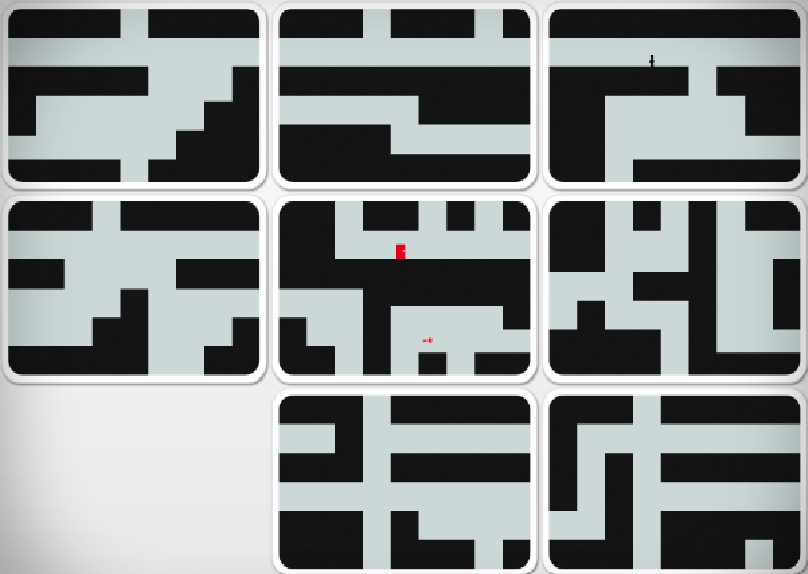
\includegraphics[scale=0.7]{resources/11/gui_original.png}
	  \end{center}
	
	A program felhasználói felületének tervezése során a felület kialakítását az egyszerűség és könnyen irányíthatóság irányelvei alakította ki. A menürendszer  felépítését az opciók minél gyorsabb elérésérére való törekvés határozta meg. Emiatt a játék közbeni lehetőségek mind elérhetőek egyetlen kattintással, vagy a megfelelő billentyű lenyomásával, gördülékenyebbé téve a játékmenetet. A fenti szempontok figyelembe vételével a felület látványterve:
	\begin{center}
		    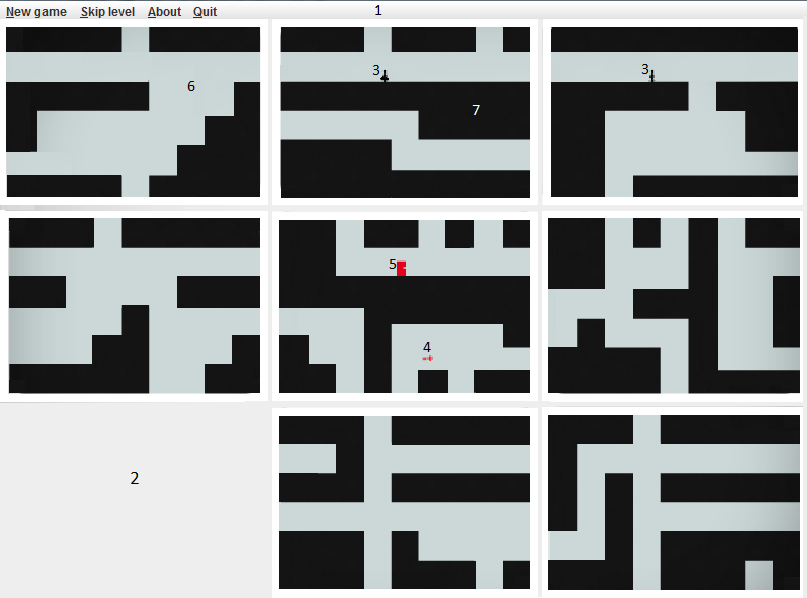
\includegraphics[scale=0.7]{resources/11/gui_own.png}
	 \end{center}
	 Az ábrán számokkal megjelölt kezelő-, és játékelemek:
	 \begin{description}	 
	  \item[1 Menüsáv] Az egyes opciók elérése.
 			\begin{description}
 			\item[1.1 New game]  Új játék kezdése.
 			\item[1.2 Skip level] A játék a következő pályára ugrik.
 			\item[1.3 About] A játék készítésével kapcsolatos információk érhetőek el.
 			\item[1.4 Quit] A játékból való kilépés.
			\end{description}
 	  \item[2 Játéktér] A folyamatban levő játék megjelenítése.
 	  \item[3 Stickmanek] A játékos által irányítható stickmanek.
 	  \item[4 Kulcs] Az ajtó nyitásához szükséges kulcs.
 	  \item[5 Ajtó] A pályáról való továbblépéshez szükséges kijárat.
 	  \item[6 Üres terület] A stickmanek által bejárható terület.
 	  \item[7 Fal] Járhatatlan szakasz.
     \end{description}

		\subsection{A grafikus rendszer architektúrája}
		%A felület m űködésének elve, a grafikus rendszer architektúrája (struktúra diagramok). A struktúra diagramokon a prototípus azon és cs ak azon osztályainak  is szerepelnie kell, amelyekhez a grafikus felületet létrehozó osztályok kapcsolódnak.
		
		\subsubsection{A felület működési elve}
		%Le kell írni, hogy a grafikai megjelenésért felelős osztályok, objektumok hogyan kapcsolódnak a meglevő rendszerhez, a megjelenítés során mi volt az alapelv. Törekedni kell az MVC megvalósításra. Alapelvek lehetnek: push  alapú: a modell értesíti a felületet, hogy változott; pull  alapú: a felület kérdezi le a modellt, hogy változott-e;  kevert: a kett ő kombinációja.
		A grafikus felület a \texttt{Game} osztály által szolgáltatott publish/subscribe mintát megvalósító kommunikációs csatornán keresztül értesül a modell változásairól. A felület továbbá ismeri az aktuális \texttt{Game} objektumot, így téve lehetővé a játék állapotának megjelenítését. Amikor a modell megváltozik, ezen a csatornán egy \texttt{invalidate} esemény érkezik, melynek hatására a megjelenésért felelős osztályok újrarajzolják a grafikus felületet. Az újrarajzolás során a grafikus felület kérdezi le a \texttt{Game} osztály állapotát (melybe beleértendő az aktuális pálya állapota és a nézet), ami alapján a rajzolást végzi.
		
		\subsubsection{A felület osztály-struktúrája}
		%Osztálydiagram. Minden új osztály, és  azon régiek, akik az újakhoz közvetlenül kapcsolódnak.
			
	    \begin{center}
		    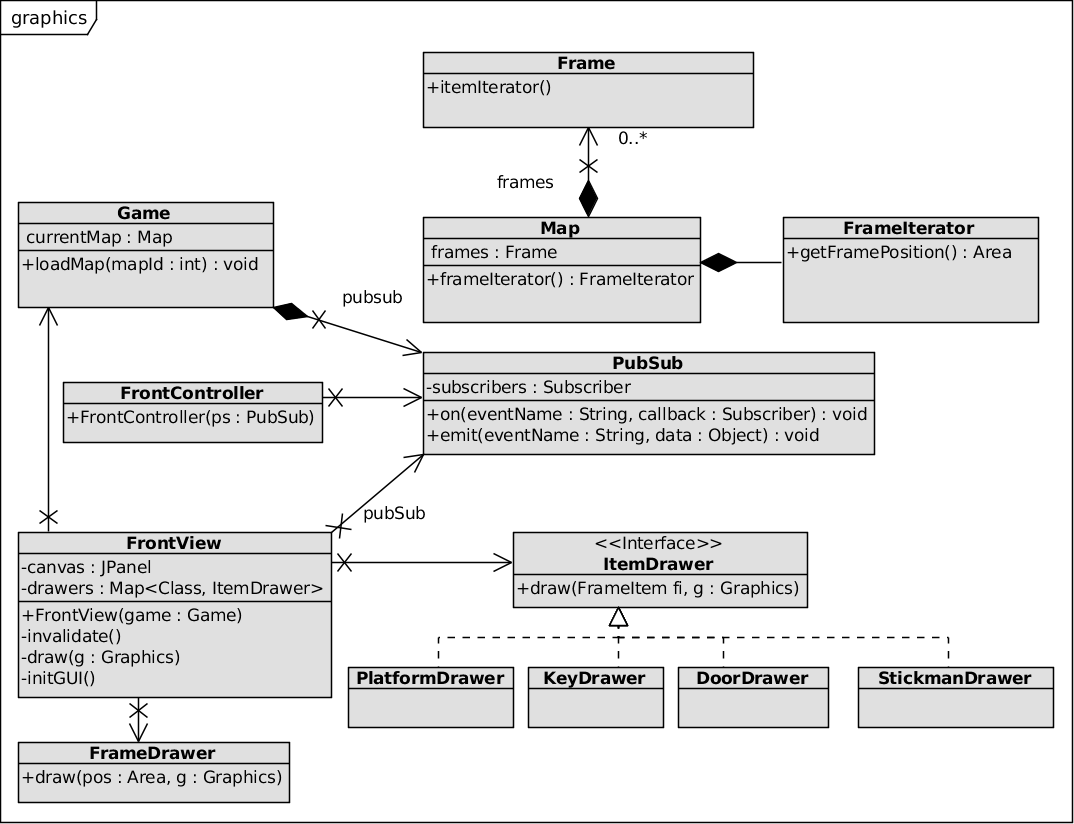
\includegraphics[scale=0.88]{resources/11/graphics.png}
	    \end{center}

	\clearpage
	\subsection{A grafikus objektumok felsorolása}
	%Az új osztályok felsorolása. Az  régi osztályok közül azoknak a  felsorolása, ahol változás volt. Ezek esetén csak a változásokat kell leírni.		
	
	%GENERATOR:CLASS_DESCRIPTIONS
		\subsubsection{DoorDrawer}
			\begin{description}

				\item[Felelősség] Ajtókat rajzol ki.

				\item[Ősosztályok] (nincs)
				\item[Interfészek] ItemDrawer.
				\item[Attribútumok] (nincs)
				\item[Metódusok]$\ $
					\begin{description}
						\item[\texttt{+draw(fi : FrameItem, g : Graphics)}] \hfill \\Kirajzolja az átadott ajtót az átadott Graphics objektumon. 
					\end{description}
			\end{description}

		\subsubsection{Frame}
			Kibővített osztály.
			\begin{description}
				\item[Metódusok]$\ $
					\begin{description}
						\item[\texttt{+itemIterator() : Iterator}] \hfill \\Visszaad egy iteratort, mely a tartalmazott  elemeken megy végig. 
					\end{description}
			\end{description}
			
		\subsubsection{FrameDrawer}
			\begin{description}

				\item[Felelősség] Kereteket rajzol ki.

				\item[Ősosztályok] (nincs)
				\item[Interfészek] (nincs)
				\item[Attribútumok] (nincs)
				\item[Metódusok]$\ $
					\begin{description}
						\item[\texttt{+draw(f : Frame, g : Graphics)}] \hfill \\Kirajzol egy keretet 
					\end{description}
			\end{description}

		\subsubsection{FrontController}
			\begin{description}

				\item[Felelősség] Felhasználói parancsok fogadása, értelemezése, továbbítása.

				\item[Ősosztályok] (nincs)
				\item[Interfészek] (nincs)
				\item[Attribútumok]$\ $
					\begin{description}
						\item[\texttt{-pubSub : PubSub}]Kommunikációs csatorna a Game felé.
					\end{description}
				\item[Metódusok] (nincs)
			\end{description}
			
		\subsubsection{FrontView}
			\begin{description}

				\item[Felelősség] Kirajzolja a pálya aktuális állapotát, a benne lévő keretekkel, elemekkel stb. együtt, valamint megjeleníti a vezérlőket (pl. következő pályára lépés).

				\item[Ősosztályok] (nincs)
				\item[Interfészek] (nincs)
				\item[Attribútumok]$\ $
					\begin{description}
						\item[\texttt{-canvas : JPanel}]Az aktuális pálya megjelenítésére szolgáló terület.
						\item[\texttt{-drawers : Map}]A különböző típusú FrameItemekhez tartozó rajzoló osztályok tárolója.
						\item[\texttt{-game : Game}]A játék modellje
					\end{description}
				\item[Metódusok]$\ $
					\begin{description}
						\item[\texttt{-draw(g : Graphics)}] \hfill \\Gondoskodik a keretek és keret elemek canvaszra történő kirajzolásáról. 
						\item[\texttt{-initGUI()}] \hfill \\Inicializálja a grafikus interfészt,  többek közt megjeleníti a játékhoz tartozó ablakot. 
						\item[\texttt{-invalidate()}] \hfill \\Kezdeményezi a pálya újrarajzolását. 
					\end{description}
			\end{description}

		\subsubsection{ItemDrawer} Interfész.
			\begin{description}

				\item[Felelősség] FrameItemeteket rajzol ki.

				\item[Ősosztályok] (nincs)
				\item[Metódusok]$\ $
					\begin{description}
						\item[\texttt{+draw(fi : FrameItem, g : Graphics)}] \hfill \\Kirajzolja az átadott FrameItemet az átadott Graphics objektumon. 
					\end{description}
			\end{description}

		\subsubsection{KeyDrawer}
			\begin{description}

				\item[Felelősség] Kulcsokat rajzol ki.

				\item[Ősosztályok] (nincs)
				\item[Interfészek] ItemDrawer.
				\item[Attribútumok] (nincs)
				\item[Metódusok]$\ $
					\begin{description}
						\item[\texttt{+draw(fi : FrameItem, g : Graphics)}] \hfill \\Kirajzolja az átadott kulcsot az átadott Graphics objektumon. 
					\end{description}
			\end{description}

		\subsubsection{Map}
			Kibővített osztály.
			\begin{description}
				\item[Metódusok]$\ $
					\begin{description}
						\item[\texttt{+frameIterator() : Map.FrameIterator}] \hfill \\Visszaad egy iteratort, mellyel a tartalmazott kereteken lehet végigmenni 
					\end{description}
			\end{description}

		\subsubsection{Map.FrameIterator}
			\begin{description}

				\item[Felelősség] A mögöttes implementációtól függetlenül felsorolja a pálya által tartalmazott kereteket.

				\item[Ősosztályok] (nincs)
				\item[Interfészek] Iterator.
				\item[Attribútumok]$\ $
					\begin{description}
						\item[\texttt{-currentColumnIterator : Iterator}]Aktuális oszlop iteratora
						\item[\texttt{-currentRowIndex : int}]Aktuális sor indexe
						\item[\texttt{-nextColumnIndex : int}]Következő oszlop indexe
					\end{description}
				\item[Metódusok]$\ $
					\begin{description}
						\item[\texttt{+getFramePosition() : Area}] \hfill \\Megadja az aktuális keret által elfoglalt  pozíciót a pálya keretrácsában.    A bal felső sarokban a x:0, y:0  pozíciójú keret található. 
						\item[\texttt{-getNextColumn() : List}] \hfill \\Váltás a következő oszlopra 
						\item[\texttt{+hasNext() : boolean}] \hfill \\Ellenőrzi, hogy van-e még bejáratlan keret 
						\item[\texttt{+next() : Frame}] \hfill \\Lépés a következő keretre 
					\end{description}
			\end{description}
			
		\subsubsection{PlatformDrawer}
			\begin{description}

				\item[Felelősség] Platformokat rajzol ki.

				\item[Ősosztályok] (nincs)
				\item[Interfészek] ItemDrawer.
				\item[Attribútumok] (nincs)
				\item[Metódusok]$\ $
					\begin{description}
						\item[\texttt{+draw(fi : FrameItem, g : Graphics)}] \hfill \\Kirajzolja az átadott platformot az átadott Graphics objektumon. 
					\end{description}
			\end{description}

		\subsubsection{StickmanDrawer}
			\begin{description}

				\item[Felelősség] Stickmaneket rajzol ki.

				\item[Ősosztályok] (nincs)
				\item[Interfészek] ItemDrawer.
				\item[Attribútumok] (nincs)
				\item[Metódusok]$\ $
					\begin{description}
						\item[\texttt{+draw(fi : FrameItem, g : Graphics)}] \hfill \\Kirajzolja az átadott stickmant az átadott Graphics objektumon. 
					\end{description}
			\end{description}
%GENERATOR:CLASS_DESCRIPTIONS

	\clearpage
	\subsection{Kapcsolat az alkalmazói rendszerrel}
	%Szekvencia-diagramokon ábrázolni kell a grafikus rendszer működését. Konzisztens kell legyen az el őz ő alfejezetekkel. Minden metódus,  ami ott szerepel, fel kell tűnjön valamelyik szekvenciában. Minden metódusnak, ami szekvenciában  szerepel, szereplnie kell a valamelyik osztálydiagramon.
		\subsubsection{Initialize}
		    \begin{center}
			    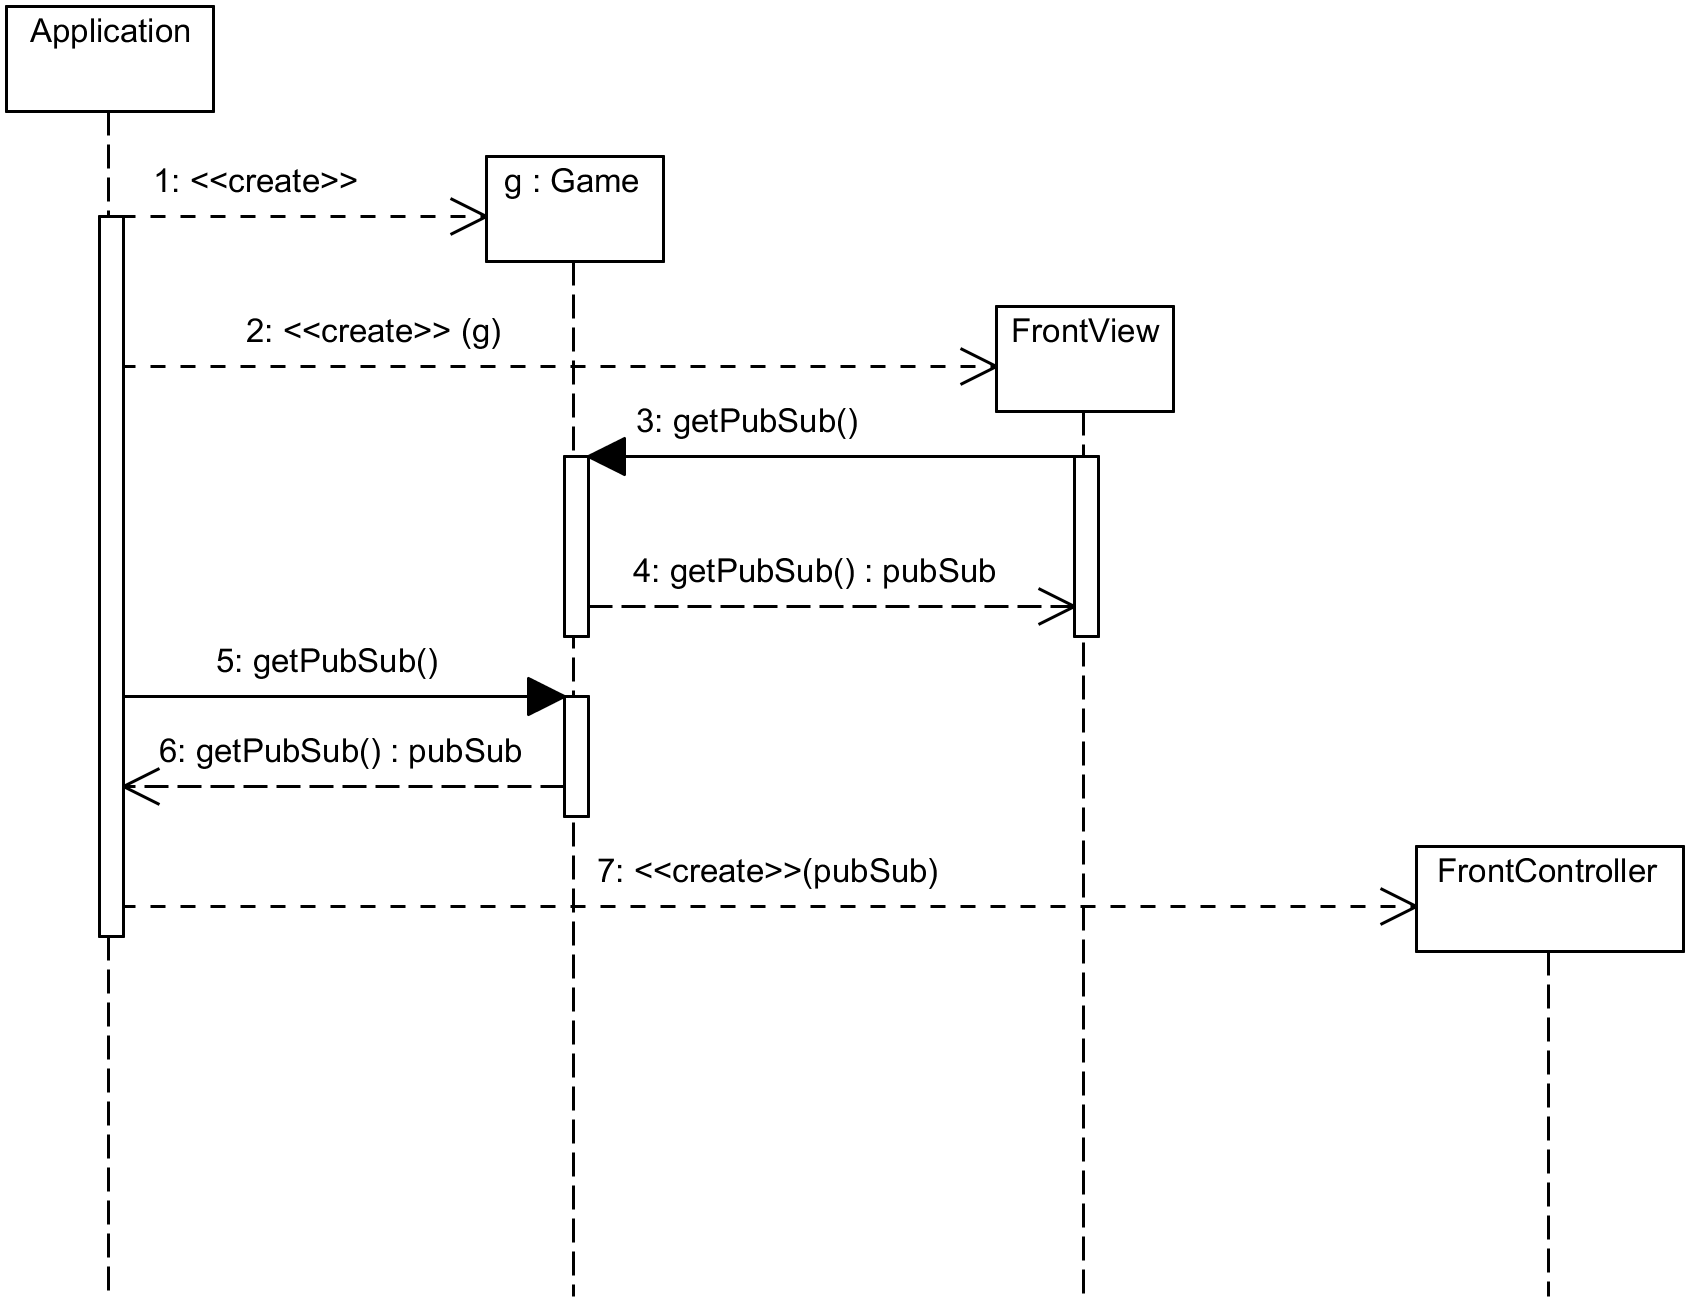
\includegraphics[scale=0.88]{resources/11/init.png}
		    \end{center}

		\subsubsection{Event}
		    \begin{center}
			    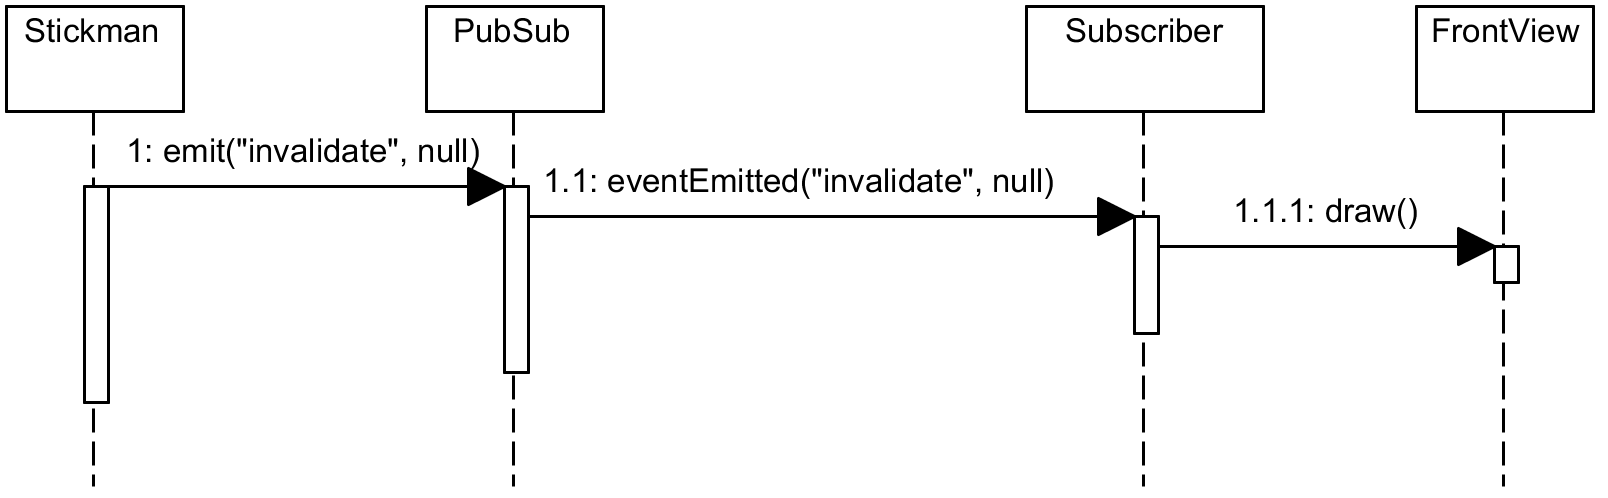
\includegraphics[scale=0.88]{resources/11/event.png}
		    \end{center}

		\subsubsection{Kirajzolás}
		    \begin{center}
			    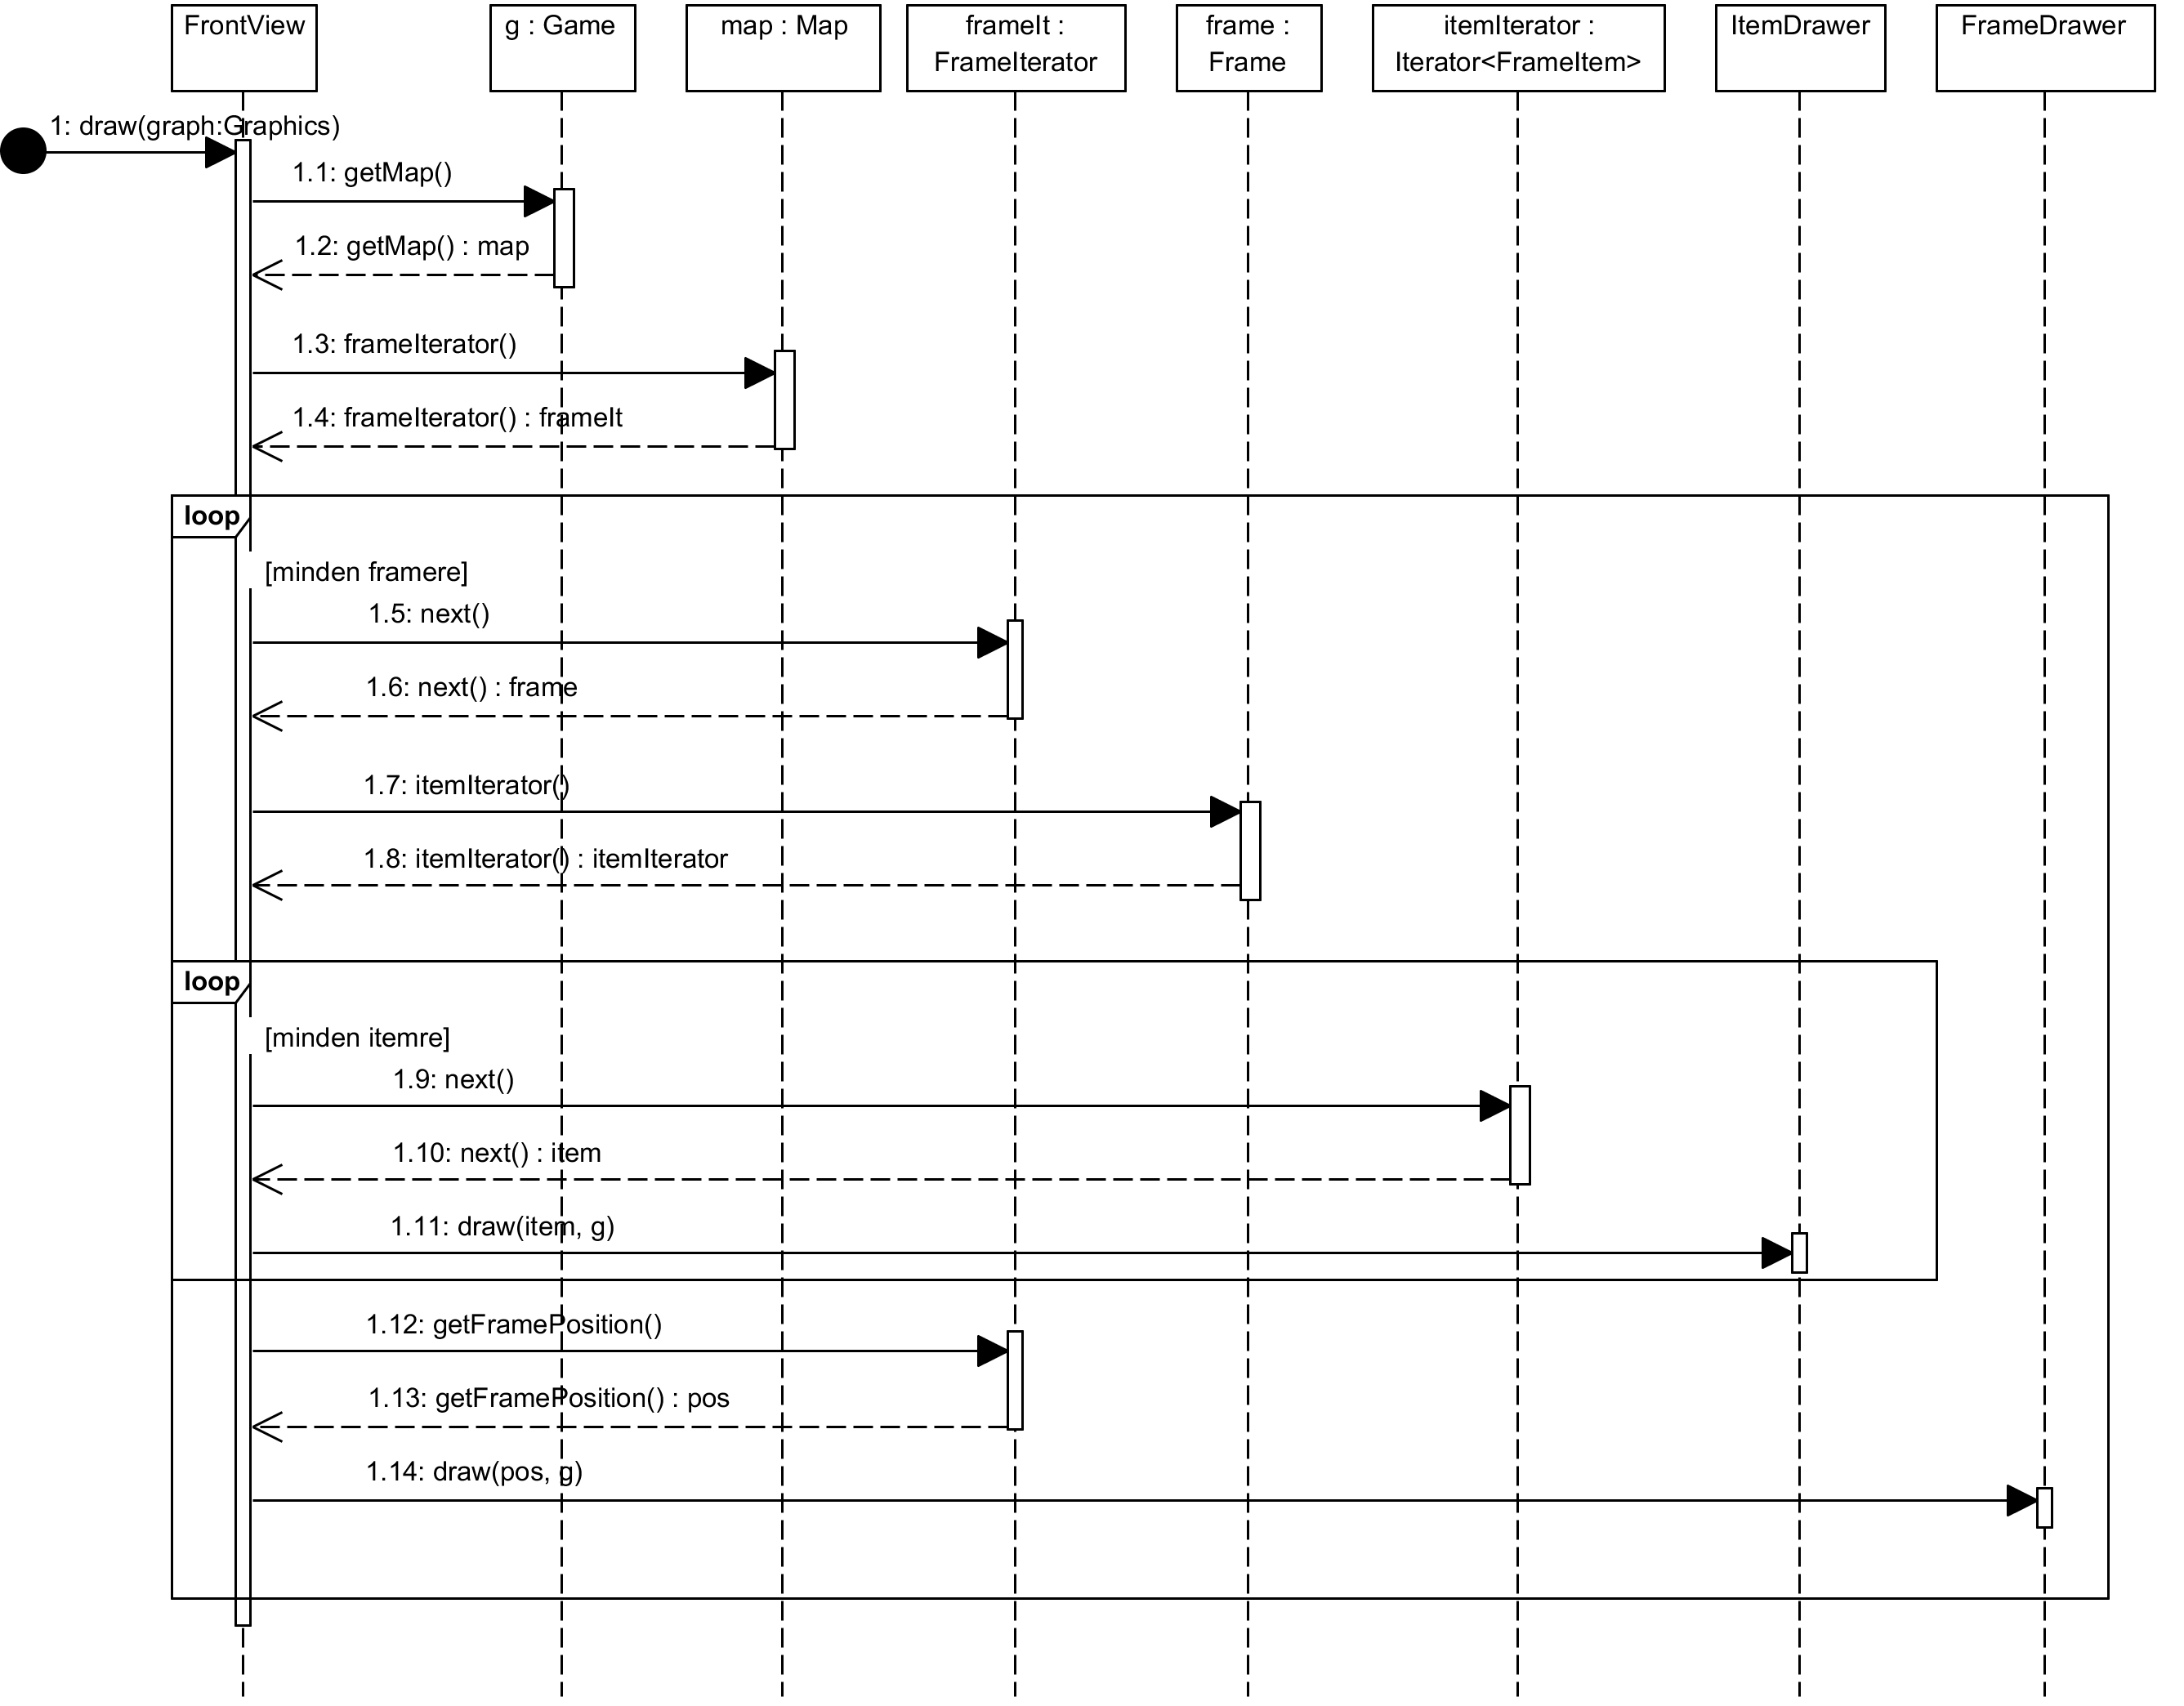
\includegraphics[scale=0.95, angle=-90]{resources/11/drawing.png}
		    \end{center}
	
		\subsection{Napló}
	% The diary generator uses the following comments to identify the beginning and the ending of the generated diary
	% The following content is auto generated, please do NOT modify, edit the related shared document instead.
	%GENERATOR:DIARY
    \begin{center} 
        \begin{tabular}{| l | p{1.9cm} | p{2.6cm} | p{6.1cm} |}
            \hline
                Kezdet & Időtartam & Résztvevők & Leírás \\
            \hline \hline 
2012. 04. 16. 17:00 & 1.5 óra & Thaler & Utólagos javítások\\ \hline
2012. 04. 21. 22:00 & 0.5 óra & Kádár & Dokumentáció előkészítése\\ \hline
2012. 04. 22. 11:30 & 3 óra & Thaler & A grafikus interfész doc.\\ \hline
2012. 04. 22. 15:15 & 2.5 óra & Kádár & Szekvencia\\ \hline
2012. 04. 22. 15:15 & 3 óra & Berki & Grafikus interfész, dokumentáció\\ \hline
2012. 04. 22. 18:45 & 3.5 óra & Fodor & Osztály dokumentáció\\ \hline
2012. 04. 22. 23:00 & 1.5 óra & Thaler & Osztálydiagram, dokumentáció\\ \hline
2012. 04. 22. 23:30 & 0.5 óra & Kádár & Szekvencia javítás\\ \hline
2012. 04. 23. 8:00 & 1 óra & Berki & Nyomtatás, átnézés\\ \hline
2012. 04. 22. 23:00 & 0.5 óra & Fodor & Átnézés\\ \hline

            \hline
        \end{tabular}
    \end{center}
%GENERATOR:DIARY
\newpage
\section{Grafikus változat beadása}

	\subsection{Fordítási és futtatási útmutató}
		%A feltöltött program fordításával és futtatásával kapcsolatos útmutatás. Ennek tartalmaznia kell leltárszer űen az egyes fájlok pontos nevét, méretét byte-ban, keletkezési idejét, valamint azt, hogy a fájlban mi került megvalósításra.
		
		\subsubsection{Fordítás és telepítés}
			%A fenti listában szerepl ő forrásfájlokból milyen műveletekkel lehet a biná ris, futtatható kódot el őállítani, milyen műveletek elvégzése szükséges a telepítéshez. Az előállításhoz csak a 2. Követelmények c. dokumentumban leírt környezetet szabad előírni.
			
		 A fordítás batch fájl segítségével történik. Nyissunk meg egy parancssort, ahol a Java fájlok futtatásához szükséges környezeti változók be vannak állítva (JDK Command Prompt). A könyvtárszerkezet gyökérmappájában állva adjuk ki a \texttt{tools\textbackslash gui\_build.bat} utasítást. Ennek hatására megtörténik a forrásfájlok lefordítása, melyről egy értesítés jelenik meg a képernyőn.

		\subsubsection{Futtatás}
			% A futtatható, telepített rendszer elindításával kapcsolatos teend ők leírása. Az indításhoz csak a 2. Követelmények c. dokumentumban leírt környezetet szabad előírni.	
		
		A fordítás után lehetőségünk nyílik a program futtatására. Ez szintúgy batch fájl segítségével történik a fenti módhoz hasonlóan. \\ A program futtatásához adjuk ki a \texttt{tools\textbackslash gui\_run.bat} utasítást.
		
		\paragraph*{Irányítás -- billentyűk}
		A program alapértelmezetten távoli nézetben indul, melyről a jobb felső sarokban megjelenő ikon tájékoztat. Ebben a nézetben a kurzorok használhatóak a keretek mozgatásához. Közeli nézetbe a szóköz lenyomásával lehet jutni. Ebben a nézetben az első stickman (lány) mozgatására a kurzorok, a második stickman (fiú) mozgatására a \emph{wasd} billentyűk használhatóak.

		\subsubsection{Fájllista}
			\begin{center}
			    \begin{tabular}{ | l | l | l | p{5cm} |}
				    \hline
				    \textbf{Fájl neve}	& \textbf{Méret}	& \textbf{Keltezés ideje}	& \textbf{Tartalom} \\ \hline
				    %Autogenerated content, do not modify
                    %GENERATOR:FILE_LIST
						key\_collected.png		&	194 bytes	&	2012. 05. 06. 22:10:30	&	Megtalált kulcs\\ \hline
						key.png		&	184 bytes	&	2012. 05. 06. 21:12:36	&	Kulcs\\ \hline
						stickman1.png		&	226 bytes	&	2012. 05. 06. 21:12:36	&	Első játékos\\ \hline
						door.png		&	186 bytes	&	2012. 05. 06. 21:12:36	&	Ajtó\\ \hline
						stickman2.png		&	216 bytes	&	2012. 05. 06. 21:12:36	&	Második játékos\\ \hline
						map\_1		&	204 bytes	&	2012. 05. 06. 21:12:36	&	Első pálya\\ \hline
						map\_2		&	394 bytes	&	2012. 05. 06. 21:12:36	&	Második pálya\\ \hline
						map\_3		&	271 bytes	&	2012. 05. 06. 21:12:36	&	Harmadik pálya\\ \hline
						map\_4		&	727 bytes	&	2012. 05. 07. 08:16:52	&	Negyedik pálya\\ \hline
						Application.java		&	817 bytes	&	2012. 05. 06. 11:08:57	&	Application osztály	\\ \hline
						Key.java		&	1690 bytes	&	2012. 04. 07. 23:49:03	&	Key osztály	\\ \hline
						Platform.java		&	958 bytes	&	2012. 04. 01. 22:58:45	&	Platform osztály	\\ \hline
						Timer.java		&	1744 bytes	&	2012. 05. 06. 11:08:57	&	Timer osztály	\\ \hline
						Door.java		&	1207 bytes	&	2012. 04. 15. 23:38:51	&	Door osztály	\\ \hline
						Map.java		&	15508 bytes	&	2012. 05. 04. 22:32:08	&	Map osztály	\\ \hline
						DIRECTION.java		&	332 bytes	&	2012. 04. 01. 20:38:59	&	DIRECTION osztály	\\ \hline
						MapFactory.java		&	5107 bytes	&	2012. 04. 14. 23:31:46	&	MapFactory osztály	\\ \hline
						Frame.java		&	11287 bytes	&	2012. 05. 03. 20:36:05	&	Frame osztály	\\ \hline
			    \end{tabular}
			\end{center}	
			
			%pagebreak					
			
			\begin{center}
			    \begin{tabular}{ | l | l | l | p{5cm} |}
				    \hline
				    \textbf{Fájl neve}	& \textbf{Méret}	& \textbf{Keltezés ideje}	& \textbf{Tartalom} \\ \hline						
						MapErrorException.java		&	562 bytes	&	2012. 04. 01. 23:10:44	&	MapErrorException osztály	\\ \hline
						MapNotFoundException.java		&	225 bytes	&	2012. 04. 01. 23:11:31	&	MapNotFoundException osztály	\\ \hline
						Game.java		&	6783 bytes	&	2012. 05. 06. 21:12:36	&	Game osztály	\\ \hline
						PubSub.java		&	1758 bytes	&	2012. 05. 07. 08:16:52	&	PubSub osztály	\\ \hline
						AbstractFrameItem.java		&	2420 bytes	&	2012. 04. 14. 16:31:47	&	AbstractFrameItem osztály	\\ \hline
						Stickman.java		&	6153 bytes	&	2012. 05. 06. 11:08:57	&	Stickman osztály	\\ \hline
						VIEWPORT\_STATE.java		&	220 bytes	&	2012. 04. 01. 23:21:53	&	VIEWPORT\_STATE osztály	\\ \hline
						Subscriber.java		&	509 bytes	&	2012. 04. 01. 20:38:59	&	Subscriber osztály	\\ \hline
						Area.java		&	4076 bytes	&	2012. 05. 04. 21:48:24	&	Area osztály	\\ \hline
						FrameItem.java		&	1854 bytes	&	2012. 04. 14. 16:31:00	&	FrameItem osztály	\\ \hline
						ItemDrawer.java		&	424 bytes	&	2012. 04. 22. 23:26:45	&	ItemDrawer osztály	\\ \hline
						FrontView.java		&	7058 bytes	&	2012. 05. 07. 08:16:52	&	FrontView osztály	\\ \hline
						DoorDrawer.java		&	998 bytes	&	2012. 05. 07. 08:16:52	&	DoorDrawer osztály	\\ \hline
						KeyDrawer.java		&	1310 bytes	&	2012. 05. 07. 08:16:52	&	KeyDrawer osztály	\\ \hline
						StickmanDrawer.java		&	1335 bytes	&	2012. 05. 07. 08:16:52	&	StickmanDrawer osztály	\\ \hline
						PlatformDrawer.java		&	573 bytes	&	2012. 05. 03. 20:36:05	&	PlatformDrawer osztály	\\ \hline
						FrameDrawer.java		&	1411 bytes	&	2012. 05. 03. 20:36:05	&	FrameDrawer osztály	\\ \hline
						FrontView.java		&	7044 bytes	&	2012. 05. 06. 11:08:57	&	FrontView osztály	\\ \hline
						Logger.java		&	1150 bytes	&	2012. 04. 16. 00:32:01	&	Logger osztály	\\ \hline
						FrontController.java		&	6008 bytes	&	2012. 05. 07. 08:16:52	&	FrontController osztály	\\ \hline
						LoadMap.java		&	325 bytes	&	2012. 04. 14. 16:17:45	&	LoadMap osztály	\\ \hline
						MoveFrame.java		&	369 bytes	&	2012. 04. 14. 16:19:01	&	MoveFrame osztály	\\ \hline
						ViewportSwitch.java		&	296 bytes	&	2012. 04. 14. 16:18:10	&	ViewportSwitch osztály	\\ \hline
						Timer.java		&	574 bytes	&	2012. 04. 14. 17:14:21	&	Timer osztály	\\ \hline
						FrontController.java		&	3572 bytes	&	2012. 04. 16. 01:10:56	&	FrontController osztály	\\ \hline
						Command.java		&	2874 bytes	&	2012. 04. 14. 16:16:19	&	Command osztály	\\ \hline
						InvalidArgumentException.java		&	590 bytes	&	2012. 04. 14. 16:07:57	&	InvalidArgumentException osztály	\\ \hline
						Tick.java		&	554 bytes	&	2012. 04. 14. 16:16:50	&	Tick osztály	\\ \hline
						Move.java		&	435 bytes	&	2012. 04. 14. 16:41:47	&	Move osztály	\\ \hline
						gui\_run.bat		&	58 bytes	&	2012. 05. 06. 22:10:30	&	Program futtatása\\ \hline
						gui\_build.bat		&	487 bytes	&	2012. 05. 07. 08:16:52	&	Program fordítása\\ \hline

					%GENERATOR:FILE_LIST
			    \end{tabular}
			\end{center}

	\subsection{Értékelés}
		\begin{center}
		    \begin{tabular}{ | l | c |}
			    \hline
			    \textbf{Tag neve}	& \textbf{Munka százalékban} 	\\ \hline
				Berki Endre			& 25\%							\\ \hline			    
			    Fodor Bertalan		& 25\%							\\ \hline
			    Kádár András		& 25\%							\\ \hline
			    Thaler Benedek		& 25\%							\\ \hline
		    \end{tabular}
		\end{center}
		
	\subsection{Napló}
	% The diary generator uses the following comments to identify the beginning and the ending of the generated diary
	% The following content is auto generated, please do NOT modify, edit the related shared document instead.
	%GENERATOR:DIARY
    \begin{center} 
        \begin{tabular}{| l | p{1.9cm} | p{2.6cm} | p{6.1cm} |}
            \hline
                Kezdet & Időtartam & Résztvevők & Leírás \\
            \hline \hline 
2012. 04. 27. 8:15 & 0.5 óra & Thaler & Organizáció\\ \hline
2012. 04. 30. 11:30 & 0.5 óra & Kádár & Tex inicializáció\\ \hline
2012. 04. 30. 12:00 & 3 óra & Kádár & Fájllista generátor\\ \hline
2012. 05. 02. 23:00 & 1 óra & Thaler & Support\\ \hline
2012. 05. 03. 16:45 & 0.5 óra & Kádár & Map készítés\\ \hline
2012. 05. 01. 15:00 & 4 óra & Fodor & Grafikus felület kódolása: felépítés, rajzolás\\ \hline
2012. 05. 02. 22:30 & 2 óra & Fodor & Grafikus felület kódolása\\ \hline
2012. 05. 03. 19:00 & 0.5 óra & Fodor & Grafikus felület kódolása\\ \hline
2012. 05. 05. 16:30 & 3 óra & Fodor & Grafikus felület kódolása: kontroller\\ \hline
2012. 05. 05. 14:30 & 2 óra & Thaler & Hibajavítások\\ \hline
2012. 05. 05. 19:30 & 1.5 óra & Fodor & Kódbeli javítások\\ \hline
2012. 05. 06. 19:50 & 0.5 óra & Kádár & Mapok\\ \hline
2012. 05. 06. 15:50 & 3 óra & Berki & Grafikák elkészítése\\ \hline
2012. 05. 06. 19:20 & 0.5 óra & Fodor & Grafikák beillesztése\\ \hline
2012. 05. 06. 20:30 & 0.5 óra & Fodor & Javítások\\ \hline
2012. 05. 06. 20:45 & 1 óra & Berki & Dokumentáció, tesztelés\\ \hline
2012. 05. 06. 23:10 & 2 óra & Fodor & Javítások\\ \hline
2012. 05. 06. 21:00 & 3 óra & Thaler & Javítás, csomagolás\\ \hline
2012. 05. 06. 8:00 & 1 óra & Thaler & Dokumentáció zárása, csomagolás\\ \hline
2012. 05. 06. 9:30 & 0.5 óra & Berki & Átnézés, nyomtatás\\ \hline

            \hline
        \end{tabular}
    \end{center}
%GENERATOR:DIARY

	
\end{document}
